\documentclass[12pt,twoside]{report}
\usepackage[utf8]{inputenc}
\usepackage{graphicx}
\graphicspath{ {images/} }
\usepackage[a4paper,width=150mm,top=25mm,bottom=25mm,bindingoffset=6mm]{geometry}
\usepackage{wrapfig}
\usepackage{lscape}
\usepackage{rotating}
\usepackage{epstopdf}
\usepackage{listings}

% package used by \citep and \citet
\usepackage[sort&compress,comma,authoryear]{natbib}
\usepackage[options ]{algorithm2e}
\usepackage{url}
\def\UrlBreaks{\do\/\do-}
\usepackage{breakurl}
\usepackage[breaklinks]{hyperref}
\usepackage{setspace}
\usepackage{amsmath}
\usepackage{booktabs}
\usepackage{fancyhdr}
\usepackage[acronym, toc]{glossaries} 
\makeglossaries

\newacronym{am}{AM}{Acoustic Model}
\newacronym{asr}{ASR}{Automatic Speech Recognition}
\newacronym{birnn}{Bi-RNN}{Bi-directional Recurrent Neural Network}
\newacronym{bleu}{BLEU}{BiLingual Evaluation
Understudy}
\newacronym{cfg}{CFG}{Context Free Grammar}
\newacronym{cmu}{CMU}{Carnegie Mellon University}
\newacronym{cmvn}{CMVN}{Cepstral Mean Variance Normalisation}
\newacronym{cmn}{CMN}{Cepstral Mean Normalisation}
\newacronym{cnn}{CNN}{Convolutional Neural Network}
\newacronym{ctc}{CTC}{Connectionist Temporal Classification}
\newacronym{dbn}{DBN}{Deep Belief Network}
\newacronym{dct}{DCT}{Discrete Cosine Transform}
\newacronym{dnn}{DNN}{Deep Neural Network}
\newacronym{dnns}{DNNs}{Deep Neural Networks}
\newacronym{dsn}{DSN}{Deep Scattering Network}
\newacronym{dtw}{DTW}{Dynamic Time Warping}
\newacronym{espnet}{ESPNet}{End-to-End Speech Neural Network Toolkit}
\newacronym{fsg}{FSG}{Finite-State Grammar}
\newacronym{fsgs}{FSGs}{Finite-State Grammars}
\newacronym{fst}{FST}{Finite-State Transducer}
\newacronym{gan}{GAN}{Generative Adversarial Network}
\newacronym{gmm}{GMM}{Gaussian Mixture Model}
\newacronym{gru}{GRU}{Gated Recurrent Unit}
\newacronym{hlda}{HLDA}{Heteroscedastic Linear Discriminant Analysis}
\newacronym{hmm}{HMM}{Hidden Markov Model}
\newacronym{idft}{IDFT}{Inverse Discrete Cosine Transform}
\newacronym{lda}{LDA}{Linear Discriminant Analysis}
\newacronym{lm}{LM}{Language Model}
\newacronym{lpc}{LPC}{Linear Predictive Coding}
\newacronym{llc}{LLC}{Language Learning Companion}
\newacronym{lstm}{LSTM}{Long Short-Term Memory}
\newacronym{mfcc}{MFCC}{Mel Frequency Cepstral Coefficients}
\newacronym{mfsc}{MFSC}{Mel Frequency Spectral Coefficients}
\newacronym{ml}{ML}{Machine Learning}
\newacronym{mllt}{MLLT}{Maximum Likelihood Linear Transformation}
\newacronym{mlp}{MLP}{Multi Layer Perceptron}
\newacronym{mlps}{MLPs}{Multi Layer Perceptrons}
\newacronym{oov}{OOV}{"out Of vocabulary"}
\newacronym{plp}{PLP}{Perceptual Linear Prediction}
\newacronym{rasta}{RASTA}{RelAtive SpecTrAl}
\newacronym{rbm}{RBM}{Restricted Boltzmann Machine}
\newacronym{rnn}{RNN}{Recurrent Neural Network}
\newacronym{rnns}{RNNs}{Recurrent Neural Networks}
\newacronym{sgmm}{SGMM}{Sub-space Gaussian Mixture Model}
\newacronym{sgd}{SGD}{Stochastic Gradient Descent}
\newacronym{stc}{STC}{Semi-Tied Co-variance matrix}
\newacronym{vtln}{VTLN}{Vocal Tract Length Normalisation}
\newacronym{wfst}{WFST}{Weighted  Finite State Transducer}
\newglossaryentry{latex}
{
    name=latex,
    description={Is a mark up language specially suited for scientific documents}
}

\newglossaryentry{maths}
{
    name=mathematics,
    description={Mathematics is what mathematicians do}
}

\newglossaryentry{formula}
{
    name=formula,
    description={A mathematical expression}
}



\pagestyle{fancy}
\fancyhead{}
\fancyhead[RO,LE]{Deep Scattering and End-to-End Speech Models towards Low Resource Speech Recognition}
\fancyfoot{}
\fancyfoot[LE,RO]{\thepage}
\fancyfoot[LO,CE]{Chapter \thechapter}
\fancyfoot[CO,RE]{I. J. Alamina}
\renewcommand{\headrulewidth}{0.4pt}
\renewcommand{\footrulewidth}{0.4pt}

\title{
    {Deep Scattering and End-to-End Speech Models towards Low Resource Speech Recognition}\\
    {
\includegraphics{university.png}\\
A thesis submitted to the University of Huddersfield in partial fulfilment of the requirements for the degree of Doctor of Philosophy}
}


\author{Iyalla John Alamina}
\date{January 8, 2020}

\begin{document}

\maketitle
\spacing{1.5}

\addcontentsline{toc}{section}{Abstract}
\chapter*{Abstract}
This thesis investigates and acknowledges the various limitations of Deep Neural Network (DNN) techniques when applied to low resource speech recognition.   Various aspects of developing corpora for speech recognition systems are explored.  In particular various recurrent neural network (RNN) techniques were explored to implement end-to-end speech and language models (LM). Gated Recurrent Units (GRU) RNNs were used employed for the language model for a low resourced Wakirike language while bidirectional recurrent neural networks (bi-RNNs) were used to create end-to-end speech recognition model for English language.

Previous systems employed for low resource speech recognition involving deep networks included various knowledge transfer mechanisms including hybrid hidden markov models (HMM) to deep neural networks (HMM-DNN) models and those that are HMM alone-based include subspace Gaussian Mixture Models (GMMs).   These models are based on the HMM generative model and N-gram language models.  However, the model developed in this thesis makes use of an end-to-end discriminative model using the Bi-RNN acoustic/speech model augmented using speech features from a specialised light weight convolution network-the deep scattering network (DSN).  While the light weight DSN helped to reduce the training complexity, at the same time by focusing on end-to-end with Connectionist Temporal Classification (CTC) decoding, the speech model was compressed into a one step process rather than a three-step process requiring an Acoustic Model (AM), Language Model (LM) and phonetic dictionary. The research therefore shows that it is possible to use this compacting strategy in addition to augmented speech features required for speech pattern recognition by deploying deep scattering network features with  higher dimensional vectors when compared to traditional speech features. 

\addcontentsline{toc}{section}{Dedication}
\chapter*{Dedication}
To the praise and glory of our God and of His Christ.

\addcontentsline{toc}{section}{Acknowledgements}
\chapter*{Acknowledgements}
I thank the members supervisory team including Dr David Wilson and Dr Simon Parkinson for the invaluable guidance and keen interest throughout my research.  

I also acknowledge my parents (Prof. Mrs. Jane Alamina and Dr. P. T. Alamina) for immense support shown.  My wife, children (Topaz and Jade) and family members have also stood by given and given all the encouragement I could ever need.  Thank you.  Finally, to all who have said a prayer and have contributed towards my studies or well being, I am grateful to you all.

\addcontentsline{toc}{section}{Copyright Statement}
\chapter*{Copyright statement}
\renewcommand{\theenumi}{\roman{enumi}}%
\begin{enumerate}
    \item The author of this thesis (including any appendices and/or schedules to this thesis) owns any copyright in it (the “Copyright”) and s/he has given The University of Huddersfield the right to use such copyright for any administrative, promotional, educational and/or teaching purposes.
    \item Copies of this thesis, either in full or in extracts, may be made only in accordance with the regulations of the University Library. Details of these regulations may be obtained from the Librarian. This page must form part of any such copies made.
    \item The ownership of any patents, designs, trademarks and any and all other intellectual property rights except for the Copyright (the “Intellectual Property Rights”) and any reproductions of copyright works, for example graphs and tables (“Reproductions”), which may be described in this thesis, may not be owned by the author and may be owned by third parties. Such Intellectual Property Rights and Reproductions cannot and must not be made available for use without the prior written permission of the owner(s) of the relevant Intellectual Property Rights and/or Reproductions
\end{enumerate}

\tableofcontents

\addcontentsline{toc}{section}{List of Figures}
\listoffigures
 
\addcontentsline{toc}{section}{List of Tables}
\listoftables

\clearpage
 
\addcontentsline{toc}{section}{Acronyms}
\printglossary[type=\acronymtype]

\chapter{Introduction}\label{ch1_intro}
\acrfull{asr} is a subset of Machine Translation that takes a sequence of raw audio information and translates or matches it against the most likely sequence of text as would be interpreted by a human language expert.  In this thesis, Automatic Speech Recognition will also be referred to as 
ASR or speech recognition for short.

It can be argued that while \acrshort{asr} has achieved excellent performance in specific applications, much is left to be desired for general purpose speech recognition \citep{yu2016automatic}. While commercial applications like Google voice search and Apple Siri give evidence that this gap is closing, there still are yet other areas within this research space that speech recognition task is very much an unsolved problem.

It is estimated that there are close to 7,000 human languages in the world \citep{besacier2014automatic} and yet for only a fraction of this number have there been efforts made towards practical ASR systems.  The level of ASR accuracy that has been so far achieved are based on large quantities of speech data and other linguistic resources used to train models for \acrshort{asr}. These models which depend largely on pattern recognition techniques degrade tremendously  when applied to different languages other than the languages that they were trained or designed for  \citep{Rosenberg2017end,besacier2014introduction}. More specifically, the collection of sufficient amounts of linguistic resources required to create accurate models for ASR are particularly laborious and time consuming sometimes extending to decades \citep{goldman2011easyalign,stan2016alisa}.  Research, therefore, geared towards alternative approaches towards developing is ASR systems that are reproducible across languages lacking the resources required to build robust systems is apt.

\section{ASR As a Machine Learning  problem}\label{ASRMLP}
\pagestyle{plain}
\acrlong{asr} can be put into a class of Machine Learning problems described as sequence pattern recognition because an ASR attempts to discriminate a pattern from the sequence of speech utterances. 

One immediate problem realised with this definition leads us to discuss statistical speech models that address how to handle the problem described in the following paragraph.

Speech is a complex phenomena that begins as a cognitive process and ends up as a physical process \citep{becchetti1998}.  The process of automatic speech recognition attempts to reverse engineer steps back from the physical process to the cognitive process giving rise to latent variables or mismatched data or loss of information from interpreting speech information from one physiological layer to the next.

It has been acknowledged in the research community \citep{2015watanabe,deng2013machine}  that work being done in Machine Learning has enhanced the research of automatic speech recognition.   Similarly any progress made in ASR usually constitute contributions to enhancements made in the Machine Learning field.  This also may be attributed to the fact that speech recognition in itself is a sequence pattern recognition problem subclass of machine learning.  Therefore techniques within speech recognition could be applied generally to sequence pattern recognition problems at large.

The two main approaches to Machine Learning problems historically involve two methods rooted in statistical science.  These approaches are generative and discriminative models.  From a computing science perspective, the generative approach is a brute-force approach while the discriminative model uses a rather heuristic approach to Machine Learning. This chapter presents the introductory ideas behind these two approaches and establishes the motivation for the proposed models used in this research for low resource speech recognition, as well as introducing the Wakirike language as the motivating language case study.

\section{Generative-Discriminative Speech Models disambiguation}
\pagestyle{fancy}
In chapter \ref{ch2litrev}, the \acrfull{hmm} is examined as a powerful and major driver behind generative modelling of sequential data like speech.  Generative models are data-sensitive models because they are derived from the data by accumulating as many different features which can be seen and make generalisations based on observed parameters. The discriminative model, on the other hand, has a heuristic approach to form a classification.  Rather than using features of the data directly, the discriminative method attempts to parameterise the data based on initial constraints\citep{lasserre2006principled}. It is therefore concluded that the generative approach uses a bottom-to-top strategy starting with the fundamental structures to determine the overall structure, while the discriminative method uses a top-to-bottom approach starting with the big picture and then drilling down to determine the fundamental structures.

Ultimately, generative models for Machine Learning learning can be interpreted mathematically as a joint distribution that produces the highest likelihood of outputs and inputs based on a predefined decision function.  The outputs for speech recognition being the sequence of words and the inputs for speech being the audio waveform or equivalent speech sequence. More specifically,

\begin{equation}
d_y(\mathbf{x};\lambda)=p(\mathbf{x},y;\lambda)=p(\mathbf{x}|y;\lambda)p(y;\lambda)
\label{eqn1_1}
\end{equation}

where $d_y(\mathbf{x};\lambda)$ is the decision function of $y$ for data labels $\mathbf{x}$.  This joint probability expression given as $p(\mathbf{x}|y;\lambda)$ can also be expressed as the conditional probability product in equation (\ref{eqn1_1}).  In this equation, $\lambda$ predefines the nature of the distribution referred to as model parameters~\citep{deng2013machine}.

Similarly, Machine Learning discriminative models are described mathematically as the conditional probability defined by the generic decision function below:
\begin{equation}
d_y(\mathbf{x};\lambda)=p(y|\mathbf{x};\lambda)
\label{eqn1_2}
\end{equation}

It is clearly seen that the discriminative paradigm follows a much more direct approach to pattern recognition. Although this approach appears cumbersome to model, this research leans towards this direct approach.  However, what the discriminative model gains in discriminative modularity, it loses in the model parameter estimation of ($\lambda$) in equation  (\ref{eqn1_1}) and (\ref{eqn1_2}) \citep{gales2012structured}.  
 As this research investigates, although the generative process is able to generate arbitrary outputs from learned inputs, its major drawback is the direct dependence on the training data from which the model parameters are learned. Specific characteristics of various Machine Learning models are reserved for later chapters, albeit the heuristic nature of the discriminative approach, which means not directly dependent on the training data,  gains over the generative approach as discriminative models are able to better compensate for latent variables.  
 
 In the case of speech signals, the original signal is corrupt and  the intended information message attenuated when the signal undergoes physiologic transformations of the speaking and hearing process and moves from one speech production mechanism mentioned in section \ref{ASRMLP} to the next.  The theme of pattern recognition through arbitrary layers of complexity is reinforced in the notion of deep learning~\cite{deng2014deep} as an attempt to learn patterns from data at multiple levels of abstraction. Thus while shallow Machine Learning models like Hidden Markov Models (HMMs) define latent variables for fixed layers of abstraction, deep Machine Learning models handle hidden/latent information for arbitrary layers of abstraction determined heuristically.  As deep learning mechanisms are typically implemented using \acrlong{dnn}s, this work applies deep \acrlong{rnn}s as an end-to-end discriminative classifier for speech recognition.  This is a so called "end-to-end model" because it adopts the top-to-bottom Machine Learning approaches. Unlike the typical generative classifiers that require sub-word acoustic models, the end-to-end models develop algorithms at higher levels of abstraction as well as the lower levels of abstraction. In the case of the model utilised in this research, the levels of abstraction include sentence/phrase, words and character discrimination. A second advantage of the end-to-end model is that because the traditional generative models require various stages of modeling including an acoustic, language and lexicon, the end-to-end discriminating multiple levels of abstractions simultaneously only requires a single stage process, greatly reducing the quantity of resources required for speech recognition.  From a low resource language perspective this is a desirable behaviour meaning that the model can be learned from an acoustic only source without the need of an acoustic model or a phonetic dictionary.   Thus techniques involving deep learning and end-to-end modelling are proposed and have been found to be self-sufficient \citep{hannun2014deep} with modest results without a language model.  However, applying a language model was observed to serve as a correction factor further improving recognition results \citep{hannun2014deep}. 

\section{Low Resource Languages}
Another challenge observed in complex Machine Learning models for both generative as well as discriminative learning models is the data intensive nature of the work required for robust classification models. \cite{saon2015ibm} recommends around 2000 hours of transcribed speech data for robust speech recognition system. As is covered in the next chapter, for new languages, which are low in training data such as transcribed speech, there are various strategies devised for low resource speech recognition. \cite{besacier2014automatic} outlines various matrices for bench-marking low resource languages.  From the generative speech model interest perspective,  reference is made to languages having less than ideal data in transcribed speech, phonetic dictionary and a text corpus for language modelling.  For end-to-end speech recognition models interests, the data relevant for low resource evaluation is the transcribed speech and a text corpus for language modelling.  It is worth noting that it was observed in \cite{besacier2014automatic} that speaker-base often does not affect a language resource status of a language and was often observed that large speaker bases could in fact lack language/speech recognition resources and that some languages having small speaker bases did in fact have sufficient language/ speech recognition resources.

Speech recognition methods investigated in this work are motivated by the Wakirike language discussed in the next section, which is a low resource language by definition.  Thus this research looked at low research language modelling for the Wakirike language from a corpus of Wakirike text available for analysis.  However, due to the insufficiency of transcribed speech for the Wakirike language, English language was substituted and used as a control variable to study low resource effects of a language when exposed to speech models developed in this work.

\section{The Wakirike Language}
The Wakirike municipality is a fishing community comprising 13 districts in the Niger Delta area of the country of Nigeria in the West African region of the continent of Africa. The first set of migrants to Wakirike settled at the mainland town of Okrika between AD860 and AD1515 at the earliest.  These early settlers had migrated from Central and Western regions of the Niger Delta region of Nigeria.  As the next set of migrants also migrated from a similar region, when the second set of migrants met with the first settlers they exclaimed “we are not different” or “Wakirike” \citep{wakirike}.  

Although the population of the Wakirike community from a 1995 report \citep{ethnologue} is about 248,000, the speaker base is  significantly less than stipulated.  The language is classified as Niger-Congo and Ijoid languages.  The writing orthography is Latin and the language status is 5 (developing) \citep{ethnologue}.  This means that although the language is not yet an endangered language, it still isn't thriving and it is being passed on to the next generation at a limited rate.

The Wakirike language was the focus for this research.  An End-to-end deep neural network language model was built for the Wakirike language based on the availability of the new testament bible printed edition that was available for processing.  The corpus utilized for this thesis work is approximately 9,000 words.

\section{Research aim and objectives}
\startblue
In this work, we develop speech processing models and language models based on deep and recurrent neural network implementations. These models use input features which are of interest to new and low resource languages.  In particular, we develop a language model based on \acrfull{gru} for the Wakirike language and a \acrfull{birnn} speech model for the English and Italian languages.  The aim of this research is therefore to build competitive ASR systems in a resource conservative manner encompassing both system resources as well as training data.

The research objectives were as follows:
\begin{itemize}
    \item Discover fundamental tasks relating to Language learning.  In particular, speech recognition;
    \item Discover building blocks for creating ASR systems generally, and then, pain points for new languages;
    \item Build robust ASR systems using methods that also address resource concerns; and
    \item Build and evaluate resource-friendly, end-to-end ASR systems.
\end{itemize}\stopblue

Within this framework, our focus on language learning tasks was on Automatic Speech recognition while the intention was to achieve the last two objectives through one or more of the following means:
\begin{enumerate}
    \item Reduction of time to train speech models and/or ensure training completes within few hours to few days;
    \item Optimisation of sub-tasks and training architecture within the ASR pipeline;
    \item \textcolor{blue}{Observe and recommend models which perform better or train faster than others;}
    \item Make efficient use of training parallelism;
    \item \textcolor{blue}{Obtain better or close to state-of-the-art performance; and}
    \item Induce model simplicity thereby reducing training and development time without compromising performance.
\end{enumerate}

Furthermore, following the Interspeech 2015 Zero Resource Speech Challenge \citep{versteegh2015zero}, this research also fulfilled the objectives of modelling speech at sub-word, word and syntax level. The Zero Resource Speech Challenge is inspired from infants ability to construct acoustic and language models of speech in an end-to-end manner. At the word and syntax level this research develops a character-based language model that reinforces sub-word, word and syntax level speech model based on Character-Temporal-Classification CTC.

\startblue
\subsection{Research Question}
Considering the recent development of end-to-end systems facilitated by deep-learning and sequence modelling, can we combine the recent pattern recognition strides in deep scattering transform with an end-to-end sequential model that results in a simplified CNN-based but robust speech recognition system which new and low resource languages can leverage?  In addition, can supporting Speech recognition sub-systems be replaced or enhanced or simplified by sequence-oriented end-to-end deep learning models?
\stopblue

\section{Main Contribution to knowledge}
\textcolor{blue}{This work uses a character-based neural language model for the low resourced language of Wakirike.  In addition, this work implements a unique combination of end-to-end deep recurrent neural network models with a robust and state of the art audio signal processing mechanism involving a hierarchical \acrfull{dsn} to engineer high-dimensional features to compete with current acoustic and deep architectures for speech recognition. While the language model had a better perplexity score than the 5-gram baseline, the \acrshort{dsn}-\acrshort{ctc} end-to-end sequence model performed competitively but not better than the baselines with a \acrlong{wer} of 12.9\% and 76.8\%; for \acrshort{svcsr} and \acrshort{lvcsr} tasks respectively.}

\startblue
The main contributions to knowledge of this research include:
\begin{itemize}
    \item Rather than developing separate systems including \acrlong{am}, \acrlong{lm}, phonetic dictionary, aligned text and speaker related data transformation.  Systems developed in this research uses a single end-to-end frame-work which does not require separate sub-system training only input audio and output text sequences for training.
    \item Detailed alignment of text and speech is not required only rough alignment comprising of segmented utterances and equivalent text
    \item Our system is enhanced with a robust character-based \acrlong{rnnlm} which is trained integrally within the super end-to-end model.
    \item Contribution to the Zero Resource challenge \citep{versteegh2015zero} in terms of sub-word modelling of speech features using lightweight \acrfull{dsn} and modelling of syntax level speech with end-to-end speech modelling.  This uses sequential model which simulates speech at the syntax level as opposed to the word-level.
    \item This research also implemented hybrid model subsystems based on alternative sequential models specifically for the wakirike language including
\begin{enumerate}
    \item Wakirike Diacritic text converter from plain Wakirike text 
    \item Phonetic Dictionary for Wakirike language
\end{enumerate}
    \item This research also as a pilot study designed an unsupervised syllable-phone recogniser using auto-correlation and \acrfull{gmm}
\end{itemize}


\section{Scope of the study}
This study acknowledged from the onset that it may not be able to gather the data required to build ASR systems for the Wakirike language as this is an initial problem this work hopes to get a step closer to solving.  As a result, the English and Italian languages were substituted and simulated low resource constraints by reducing the amount of hours of recorded speech data for training or reducing the vocabulary size.  This provides a rough estimate of how much of the target Wakirike language speech data will be required to provide equivalent results based on this multilingual approach.
\stopblue

\section{Thesis outline}
The engineered systems, methods and supporting literature contained in this thesis report follows the following outline and describe the research outputs of an end-to-end speech recogniser and develops the theory based on the building blocks of the research outputs.

Chapter two introduces the speech recognition pipeline and the generative speech model.  Chapter two also outlines the weaknesses in the generative model and describes some of the Machine Learning techniques applied to improve speech recognition performance.  The methods and techniques and description of the various tools and metrics for analysis of the research outputs are described and examined in Chapter three.

Various Low speech recognition methods are reviewed and the relevance of this study is also highlighted.  Chapter four describes \acrfull{rnns}. Starting with \acrfull{mlps}, we go on to specialised recurrent neural networks including \acrfull{lstm} networks and the \acrfull{gru} are detailed. These recurrent neural network units form building blocks of the language model for Wakirike language implemented in this work.

Chapter five explains the wavelet theorem as well as the deep scattering spectrum. The chapter develops the theory from Fourier transform and details the significance of using the scattering transform as a feature selection mechanism for low resource recognition.  

Chapters six and seven give descriptions of the models developed by this thesis and details the experimental setup along with the results obtained. Chapter eight is the conclusion of the work and recommendations for further study. 

\section{Chapter Summary}
Amidst seeming large success of speech-to-text technology referred to as \acrfull{asr}, there are still areas in which ASR technology struggles to perform up to the minimum acceptable level.  Situations such as very noisy environments and far field speech recognition constitute common physical scenarios where \acrshort{asr} performance degrades significantly.  Another non-physical area in which \acrshort{asr} falls short of acceptable performance and chosen as the focus of this research is the area of low-resource speech recognition.  This is the scenario where languages not rich in linguistic resources are unable to use existing resources and algorithms used in languages rich in linguistic and ASR resources, to perform automatic speech recognition. 

As this chapter identifies, the ASR problem is traditionally a \acrlong{ml} problem that models   speech production, transmission and perception and speech models are trained from language-specific data. While these \acrshort{ml} speech models may perform well for the languages the models were trained for, when introduced to a different language, having a different set of learning features, these pre-trained models fall short of expected performances for these new languages. Moreover, if the new languages do not possess a rich set of linguistic features, including resources such as aligned speech and an online text corpus amongst others \citep{besacier2014introduction}, it becomes time-consuming and extremely laborious to develop new \acrshort{asr} models for speech recognition for these so-called \acrshort{asr} ``low-resource'' languages.

This chapter also introduces the Wakirike language as a low resource language and the motivating language for this research.  In addition, the various machine learning architectures used in this research for low resource speech recognition for the Wakirike and for English language are reviewed. In particular, \acrfull{dnns} are highlighted as choice algorithms in speech recognition, and then, the Chapter goes on to describe the research contribution and the outline of this thesis.




\chapter{Low Resource Speech Models, End-to-end models and the scattering network}\label{c02}
The speech recogniser developed in this thesis is based on an end-to-end discriminative deep recurrent neural network.  Two models were developed.  The first model is a Gated-Recurrent-Unit Recurrent Neural network (GRU-RNN) was used to develop a character-based language model, while the second recurrent neural network is a Bi-Directional Recurrent neural Network (BiRNN) used as an end-to-end speech model capable of generating word sequences based on learned character sequence outputs.  This chapter describes the transition from generative speech models to these discriminative end-to-end recurrent neural network models.  Low speech recognition strategies are also discussed and the contribution to knowledge gained by using character-based discrimination as well as introducing deep scattering features to the bi-RNN speech model is brought to light.

\section{Speech Recognition Overview}\label{Ch_2_SROverview}
Computer speech recognition takes raw audio speech and converts it into a sequence of symbols.  This can be considered as an analog to digital conversion as a continuous signal becomes discretised.  The way this conversion is done is by breaking up the audio sequence into very small packets referred to as frames and developing discriminating parameters or features for each frame. Then using the vector of features as input to the speech recogniser.  

A statistical formulation \citep{young2002htk} for the speech recogniser follows given that each discretised output word in the audio speech signal is represented as a vector sequence of frame observations defined in the set $\mathbf{O}$ such that 
\begin{equation}\mathbf{O}=\mathbf{o}_1,\mathbf{o}_2,\dots,\mathbf{o}_T.
\label{eqn_1_1_sr_inputs}
\end{equation}

At each discrete time $t$, we have an observation $\mathbf{o}_t$, which is, in itself is a vector in $\mathbb{R}^D$.  From the conditional probability, it can be formulated that certain word sequences from a finite dictionary are most probable given a sequence of observations. That is:
\begin{equation}arg\max_t\{P(w_i|\mathbf{O})\}
\label{eqn_2_2_srgen}
\end{equation}

As we describe in the next section on speech recognition challenges, there is no straightforward analysis of $P(w_i|\mathbf{O})$.  The divide and conquer strategy therefore employed uses Bayes formulation to simplify the problem.  Accordingly, the argument that maximises the probability of an audio sequence given a particular word multiplied by the probability of that word is equivalent to the original posterior probability required to solve the isolated word recognition problem. This is summarised by the following equation
\begin{equation}P(w_i|\mathbf{O})=\frac{P(\mathbf{O}|w_i)P(w_i)}{P(\mathbf{O})}
\label{eqn_2_3_bayes_sr}
\end{equation}

That is, according to Bayes’ rule, the posterior probability is obtained by multiplying a certain likelihood probability by a prior probability.  The likelihood in this case, $P(\mathbf{O}|w_i)$, is obtained from a Hidden Markov Model (HMM) parametric model such that rather than estimating the observation densities in the likelihood probability, these are obtained by estimating the parameters of the HMM model.  The HMM model explained in the next section gives a statistical representation of the latent variables of speech at a mostly acoustic level.

The second parameter in the speech model, interpreted from Bayes' formula, is the prior probability of a given word.  This aspect of the model is the language model which is reviewed in section \ref{sec_lrlm}.

\subsection{HMM-based Generative speech model}
A HMM represents a finite state machine where a process transits a sequence of states from a set of fixed states \citep{gales2008application, young2002htk}. The overall sequence of transitions will have a start state, an end state and a finite number of intermediate states all within the set of finite states.  Each state transition emits an output observation that represents the current internal state of the system.

\begin{figure}
\centering
  % Requires \usepackage{graphicx}
  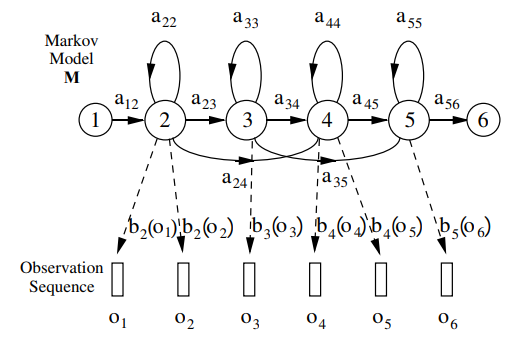
\includegraphics[width=9cm]{thesis/images/hmm}\\
  \caption{HMM Generative Model}\cite{young2002htk}\label{fig_2_1_hmm}
\end{figure}

In an HMM represented in figure \ref{fig_2_1_hmm} there are two important probabilities.  The first is the state transition probability given by $a_{ij}$ this is the probability to move from state $i$ to state $j$.  The second probability $b_j$ is the probability that an output observation is emitted when in a particular state.

Where $\mathbf{O}$, are the output observations and $M$ is the HMM.  Given that $X$ represents the sequence of states transitioned by a process, a HMM defines the joint probability of $X$ and the output probabilities given the HMM in the following representation:
\begin{equation}P(\mathbf{O}|M)=\sum_Xa_{x(0)x(1)}\prod_{t=1}^Tb_{x(t)}(\mathbf{o}_t)a_{x(t)x(t+1)}
\label{eqn_2_4_hmm}
\end{equation}

Generally speaking, the HMM formulation presents 3 distinct challenges.  The first is the likelihood of a sequence of observations given in equation \ref{eqn_2_4_hmm} above.  The next two,  described later, is the inference and the learning problem.  While the inference problem determines the sequence of steps given the emission probabilities, the learning problem determines the HMM parameters, that is the initial transition and emission probabilities of the HMM model.

For the case of the inference problem, the sequence of states can be obtained by determining the sequence of states that maximises the probability of the output sequences.

\subsection{Challenges of Speech Recognition}
The realised symbol is assumed to have a one to one mapping with the segmented raw audio speech. However, the difficulty in computer speech recognition is the fact that there is a significant amount of variation in speech that would make it practically intractable to establish a direct mapping from segmented raw speech audio to a sequence of static symbols. The phenomena known as co articulation has it that there are several different symbols having a mapping to a single waveform of speech in addition to several other varying factors including the speaker mood, gender, age, the medium of speech transduction, the room acoustics, et cetera.

Another challenge faced by automated speech recognisers is the fact that the boundaries of the words is not apparent from the raw speech waveform. A third problem that immediately arises from the second is the fact that the words from the speech may not strictly follow the words in the selected vocabulary database.  Such occurrence in speech recognition research is referred to as out of vocabulary (OOV) terms.  It is reasonable to approach these challenges using a divide and conquer strategy.  In this case, the first step would be to create assumption that somehow word boundaries can be determined.  This first step in speech recognition is referred to as the isolated word recognition case \citep{young2002htk}.

\subsection{Challenges of low speech recognition}
Speech recognition for low resource languages poses another distinct set of challenges.  In chapter one, low resource languages were described to be languages lacking in resources required for adequate machine learning of models needed for generative speech models.  These resources are described basically as a text corpus for language modelling, a phonetic dictionary and transcribed audio speech for acoustic modelling. Figure \ref{fig_2_2_asr_pipeline}, illustrates how resources required for speech recognition are utilised.  It is observed that in addition to the three resources identified other processes are required for the speech decoder to function normally.  For example, aligned speech would also need to be segmented into speech utterances to ensure that the computer resources are used conservatively.

In terms of data collection processing \cite{besacier2014automatic} enumerates the  challenges for developing low resource ASR systems to include the fact that phonologies (or language sound systems) differ across languages, word segmentation problems, fuzzy grammatical structures, unwritten languages, lack of native speakers having technical skills and the multidisciplinary nature of ASR constitute impedance to ASR system building.

\begin{figure}
\centering
  % Requires \usepackage{graphicx}
  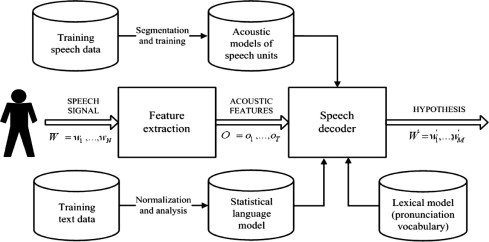
\includegraphics[width=10cm]{thesis/images/asr_pipeline}\\
  \caption{Automatic Speech Recognition Pipeline} \cite{besacier2014automatic}\label{fig_2_2_asr_pipeline}
\end{figure}

\section{Low Resource Speech Recognition}
In this system building speech recognition research, the focus was on the development of a language model and an end-to-end speech model comparable in performance to state of the art speech recognition system consisting of an acoustic model and a language model.  Low resource language and acoustic modelling is now reviewed keeping in mind that little work has been done on low-resource end-to-end speech modelling when compared to general end-to-end speech modelling and general speech recognition as a whole.  

From an engineering perspective, a practical means of achieving low resource speech modelling from a language rich in resources is through various strategies of the machine learning sub-field of transfer learning.  

Transfer learning takes the inner representation of knowledge derived from training an algorithm used from one domain and applying this knowledge in a similar domain having different set of system parameters. Early work of this nature for speech recognition is demonstrated in \citep{vu2013multilingual} where multi-layer perceptrons were used to train multiple languages rich in linguistic resources. In a later section entitled “speech recognition on a budget”, a transfer learning mechanism involving deep neural networks from \citep{kunze2017transfer} is described.

\subsection{Low Resource language modelling} \label{sec_lrlm}

General language modelling is reviewed and then Low resource language modelling is discussed in this section.  In section \ref{Ch_2_SROverview}, recall from equation \ref{eqn_2_3_bayes_sr}, the general speech model influenced by Bayes' theorem.
\begin{equation}P(w_i|\mathbf{O})=\frac{P(\mathbf{O}|w_i)P(w_i)}{P(\mathbf{O})}
\label{eqn_2_5_bayes_sr}
\end{equation}

The speech recognition model is a product of an acoustic model (likelihood probability),$P(\mathbf{O}|w_i)$ and the language model (prior probability),$P(w_i)$.  The development of  language models for speech recognition is discussed in \cite{juang2000automatic} and \cite{1996YoungA}.  

Language modelling formulate rules that predict linguistic events and can be modelled in terms of discrete density $P(W)$, where  $W=(w_1, w_2,..., w_L)$ is a word sequence. The density function $P(W)$ assigns a probability to a particular word sequence $W$.  This value determines how likely the word is to appear in an utterance. A sentence with words appearing in a grammatically correct manner is more likely to be spoken than a sentence with words mixed up in an ungrammatical manner, and, therefore, is assigned a higher probability. The order of words therefore reflect the language structure, rules, and conventions in a probabilistic way. Statistical language modeling therefore, is an estimate for $P(W)$ from a given set of sentences, or corpus.

The prior probability of a word sequence $\mathbf{w}=w_1,\dots,w_k$ required in equation (2.2) is given by:
\begin{equation}P(\mathbf{w})=\prod_{k=1}^KP(w_k|w_{k-1},\dots,w_1)
\label{eqn_c2_lm01}
\end{equation}

The N-gram model is formed by the conditioning of the word history in equation \ref{eqn_c2_lm01}.  This therefore becomes:
\begin{equation}P(\mathbf{w})=\prod_{k=1}^KP(w_k|w_{k-1},w_{k-2},\dots,w_{k-N+1})
\label{eqn_c2_lm02}
\end{equation}

N is typically in the range of 2-4.

N-gram probabilities are estimated from training corpus by counting N-gram occurrences.  This is plugged into maximum likelihood (ML) parameter estimate. For example, Given that N=3 then the probability that three words occurred is assuming $C(w_{k-2}w_{k-1}w_k)$ is the number of occurrences of the three words $C(w_{k-2}w_{k-1})$ is the count for $w_{k-2}w_{k-1}w_k$ then
\begin{equation}
P(w_k|w_{k-1},w_{k-2})\approx\frac{C(w_{k-2}w_{k-1}w_k)}{C(w_{k-2}w_{k-1})}
\label{eqn_c2_lm03}
\end{equation}

The major problem with maximum likelihood estimation scheme is data sparsity. This can be tackled by a combination of smoothing techniques involving discounting and backing-off.  The alternative approach to robust language modelling is the so-called class based models \citep{Brown1992class,Kuhn1990cache} in which data sparsity is not so much an issue.  Given that for every word $w_k$, there is a corresponding class $c_k$, then,
\begin{equation}
P(\mathbf{w})\prod_{k=1}^KP(w_k|c_k)p(c_k|c_{k-1},\dots,c_{k-N+1})
\label{eqn_c2_lm04}
\end{equation}

In 2003,  \cite{bengio2003neural} proposed a language model based on neural multi-layer perceptrons (MLPs). These MLP language models resort to a distributed representation of all the words in the vocabulary such that the probability function of the word sequences is expressed in terms of these word-level vector representations. The result of the MLP-based language models was found to be, in cases for models with large parameters, performing better than the traditional n-gram models.

Improvements over the MLPs still using neural networks over the next decade include works of \cite{mikolov2011empirical,sutskever2014sequence,luong2013better}, involved the utilisation of deep neural networks for estimating word probabilities in a language model.  While a Multi-Layer Perceptron consists of a single hidden layer, in addition to the input and output layers, a deep network, in addition to having several hidden layers, are characterised by complex structures that render the architecture beyond the basic feed forward nature. Particularly, for Recurrent Neural Network (RNN) architectures, we also have some feedback neurons in addition to the forward neurons where data flows in the reverse direction, from output to input. 

Furthermore, the probability distributions in these deep neural networks were either based upon word or sub-word models, this time having representations which also conveyed some level of syntactic or morphological weights to aid in establishing word relationships.  These learned weights are referred to as token or unit embedding \cite{pennington-etal-2014-glove}.

For the neural network implementations so far seen, a large amount of data is required due to the nature of words to have large vocabularies, even for medium-scale speech recognition applications.   \cite{kim2016character} on the other hand took a different approach to language modelling taking advantage of the long-term sequence memory of long-short-term memory cell recurrent neural network (LSTM-RNN) to model a language based on characters rather than on words.  This greatly reduced the number of parameters involved and therefore the complexity of implementation.  This method is forms the basis of the Wakirike language model implementation in this work due to the low resource constraints gains made when using a character-level language model.

Other low resource language modelling strategies employed for the purpose of speech recognition was demonstrated by \cite{xu2013cross}.  The language model developed in that work was based on phrase-level linguistic mapping from a high resource language to a low resource language using a probabilistic model implemented using a weighted finite state transducer (WFST). This method uses WFST rather than a neural network due to scarcity of training data required to develop a neural network. However, it did not gain from the high non linearity ability of a neural network model to discover hidden patterns in data, being a shallower machine learning architecture.

The language model implemented in this thesis report uses a character-based Neural network language model that employs a recurrent neural network similar to that of \cite{kim2016character}, however based on Gated Recurrent Units (GRU) RNNs \cite{cho2014learning}, for the Okrika language which is a low resource language, bearing in mind that the character level network will reduce the number of parameters required for training, just enough to develop a working language model for the purpose of speech recognition. 

\subsection{Low Resource Acoustic and speech modelling}

Two transfer learning techniques for acoustic modelling investigated by \cite{povey2011subspace} and \cite{ghoshal2013multilingual} respectively include the sub-space Gaussian mixture models (SGMMs) and the use of pretrained hidden layers of a deep neural network trained multilingually as a means to initialise weights for an unknown language.  This second method of low resource modelling has been informally referred to as the swap-hat method.

Recall that one of the challenges associated with new languages is that phonetic systems differ from one language to another.  Transfer learning approaches attempt however to recover patterns common to seemingly disparate systems and model these patterns.  

For phonetic systems, based on the premise that sounds are produced by approximate movements and positions of articulators comprising the human speech sound system is common for all humans.  It is possible to model dynamic movement from between various phones as tied state mixture of Gaussians. These dynamic states modelled using Gaussian mixture models or GMM are also called senones. \cite{povey2011subspace} postulated a method to factorize these Gaussian mixtures into a globally shared set of parameters that are non-dependent individual HMM states.  These factorisations model senones that are not represented in original data and thought to be a representation of the overall acoustic space.  While preserving individual HMM states, the decoupling of the shared space and its reuse makes SGMMs a viable candidate for transfer learning of acoustic models for new languages.

The transfer learning procedure proposed in \cite{ghoshal2013multilingual} employed the use of deep neural networks, in particular deep belief networks \citep{bengio2007greedy}.  Deep Belief Networks are pretrained, layer-wise  stacked Restricted Boltzmann Machines (RBMs)\citep{smolensky1986information}.  The output of this network trained on senones correspond to HMM context dependent states.  However, by decoupling hidden layers from outer and output layers and fine-tuned to a new language, the network is shown to be insensitive to the choice of languages analogous to global parameters of SGMMs. The 7-layer, 2000 neuron per layer network used did not utilise a bottleneck layer corresponding to triphone states trained on MFCC features \citep{grezl2008optimizing}.

\section{Groundwork for low resource end-to-end speech modelling}
The underpinning notion of this work is firstly a departure from the bottom-to-top baggage that comes as a bye-product of the generative process sponsored by the HMM-based speech models so that we can gain from simplifying the speech pipeline from acoustic, language and phonetic model to just a speech model that approximates the same process.  Secondly, the model developed seeks to overcome the data intensity barrier and was seen to achieve measurable results for GRU RNN language models.  Therefore adopting the same character-based strategy, this research performed experiments using the character-based bi-directional recurrent neural networks (BiRNN).  However, BiRNNs researchers have found them as other deep learning algorithms, as being very data intensive\cite{hannun2014deep}.  The next paragraphs introduce Deep-speech BiRNNs and the two strategies for tackling the data intensity drawback as related with low resource speech recognition.

\subsection{Deep speech}
Up until recently, speech recognition research has been centred on improvements of the HMM-based acoustic models.  This has included a departure from generative training of HMM to discriminative training \citep{woodland2000large} and the use of neural network precursors to initialise the HMM parameters \citep{mohamed2012acoustic}.  Although these  discriminative models brought improvements over generative models, being HMM dependent speech models they lacked the end-to-end nature.  This means that they were subject to training of acoustic, language and phonetic models.  With the introduction of the Connectionist Temporal Classification (CTC) loss  function, \cite{graves2014towards} finally found a means to end-to-end speech recognition departing from HMM-based speech recognition. 

The architecture of the Deep-speech end-to-end speech recognition model \cite{hannun2014first} follows an end-to-end Bi-directional Recurrent Neural Network (BiRNN) and CTC loss function \citep{graves2006connectionist}.  The CTC loss function uses a modified beam search to sum over all possible input-output sequence alignments thereby maximising the likelihood of the output sequence characters.

\subsection{Speech Recognition on a low budget}

In this section, a recent transfer learning speech model \citep{kunze2017transfer} that has some characteristics similar to the speech model developed in this thesis is reviewed.  The end-to-end speech model described by \cite{kunze2017transfer} is based on that developed by \cite{collobert2016wav2letter} and is based on deep convolutional neural networks rather than the Bi-RNN structure proposed by this work.  In addition it uses a loss function based on the AutoSegCriterion which is claimed to work competitively with raw audio waveform without any preprocessing.  The main strategy for low resource management in their system was the freezing of some layers within the convolutional network layer.  The low resource mechanisms used in this work includes the use of a unique scattering network being used as input features for the BiRNN model.  The fascinating similarity between the end-to-end BiRNN speech model developed in this work and the transfer learning model in \cite{kunze2017transfer} is the fact that the scattering network input are equivalent to the output of a light-weight convolutional neural network \cite{hannun2014first}.  Therefore the proposed system then approximates a combination of a recurrent neural network as well as a convolution neural network without the overhead of actually training a convolutional neural network (CNN).

Introduction of the unique scattering network is discussed in the next section.  It is worthy to note however that \cite{kunze2017transfer} uses a CNN network only while \citep{amodei2016deep} uses both RNN and CNN network.  The speech model in this thesis uses a BiRNN model and combines an RNN model with the scattering layer which represents a light-weight low resource friendly pseudo enhanced CNN backing.  What is meant by pseudo enhanced CNN backing is reserved for the next section, however, therefore, the proposed speech model in this thesis stands to gain from an enhanced but lightweight CNN combined with RNN learning.

\subsection{Adding a Scattering layer}

In machine learning, training accuracy is greatly improved through a process described as feature engineering.  In feature engineering, discriminating characteristics of the data is enhanced at the same time non-distinguishing features constituting noise is removed or attenuated to a barest minimum.  A lot of the components signal speech signal are due to noise in the environment as well as signal channel distortions such as losses due to conversion from audio signals to electrical signal in the recording system.

In figure \ref{fig_2_2_asr_pipeline}, feature engineering is done at the feature extraction stage of the ASR pipeline. It has been shown that a common technique using Mel-frequency cepstral coefficients (MFCCs) \citep{davis1990comparison} can represent speech in a stable fashion that approximate how the working of the human auditory speech processing and is able to filter useful components in the speech signal required for human speech hearing. Similar feature processing schemes have been developed include Perceptual Linear Prediction (PLP) \citep{hermansky1990perceptual} and RASTA \citep{hermansky1994rasta}. 

The scattering spectrum defines a locally translation invariant representation of a signal resistant to signal deformation over extended periods of time spanning seconds of the signal \citep{anden2014deep}. While Mel-frequency cepstral coefficients (MFCCs) are cosine transforms of Mel-frequency spectral coefficients (MFSCs), the scattering operator consists of a composite wavelet and modulus operation on input signals. 

Over a fixed time, MFSCs measure signal energy having constant Q bandwidth Mel-frequency intervals.  This procedure is susceptible to time-warping signal distortions since these information often reside in the high frequency regions discarded by Mel-frequency intervals.  As time-warping distortions isn't explicit classifier objective when developing these filters, there is no way to recover such information using current techniques. 

In addition, short time windows of about 20 ms are used in these feature extraction techniques since at this resolution speech signal is mostly locally stationary.  Again, this resolution adds to the loss of dynamic speech discriminating information on signal structures that are non-stationary at this time interval. To minimize this loss Delta-MFCC and Delta-Delta-MFCCs \citep{furui1986speaker} are some of the means developed to capture dynamic audio signal characterisation over  larger time scales.

By computing multi-scale co-occurrence coefficients from a wavelet-modulus operation \cite{anden2011multiscale}, show that non-stationary behaviour lost by MFSC coefficients is captured by the scattering transform multi scale co-occurrence coefficients and the scattering representation includes MFSC-like measurements.  Together with higher-order co-occurrence coefficients, deep scattering spectrum coefficients represents audio signals similar to  models based on cascades of constant-Q filter banks and rectifiers.  In particular, second-order co-occurrence coefficients carry important  signal information capable of discriminating dynamic information lost to the MFCC analog over several seconds and therefore a more efficient discriminant than the MFCC representation. Second-order co-occurrence coefficients calculated by cascading wavelet filter banks and rectified using modulus operators have been evaluated as equivalent to a light-weight convolutional neural networks whose output posteriors are computed at each layer instead of only at the output layer \cite{mallat2016understanding}.

The premise for this work is that low speech recognition can be achieved by having higher resolution features for discrimination as well as using an end-to-end framework to replace some of the cumbersome and time-consuming hand-engineered domain knowledge required in the standard ASR pipeline.  In addition, this research work makes contributions to the requirements for the two tracks specified in the Zero Resource challenge of 2015 \citep{versteegh2015zero}.  The first requirement is sub-word modelling satisfied with using deep scattering network and the second that of spoken term discovery criteria being satisfied with the end-to-end speech model supplemented with a language model.
\section{Methodology}
System building methodology \citep{nunamaker1990systems} for speech recognition systems require models to be evaluated against speech recognition machine learning metrics.  For language models, perplexity metric was used for evaluation.  Bleu has also been used as a metric for evaluating language models.

Perplexity measures the complexity of a language that the language model is designed to represent \citep{1976jelinekcontinuous}. In practice, the entropy of a language with an N-gram language model $P_N(W)$ is measured from a set of sentences and is defined as
\begin{equation}H=\sum_{\mathbf{W}\in\Omega}P_N(\mathbf{W})
\label{eqn_c2_lm05}
\end{equation}

where $\Omega$ is a set of sentences of the language. The perplexity, which is interpreted as the average word-branching factor, is defined as
\begin{equation}PP(W)=2^H
\label{eqn_c2_lm06}
\end{equation}
where H is the average entropy of the system or the average log probability defined as
\begin{equation}
H=-\frac{1}{N}\sum_{i=1}^N[log_2P(w_1,w_2\dots w_N)]
\label{eqn_c2_lm07}
\end{equation}
For a bi gram model therefore, equation (\ref{eqn_c2_lm07}) becomes
\begin{equation}
PP(W)=2^H=2^{-\frac{1}{N}\sum_{i=1}^N[log_2P(w_1,w_2\dots w_N)]}
\label{eqn_c2_lm08}
\end{equation}
After simplifying we have
\begin{equation}
PP(W)=\sqrt[N]{\prod_{i=1}^N\frac{1}{P(w_i|w_{i-1})}}
\label{eqn_c2_lm09}
\end{equation}


Full speech recognition pipelines are usually evaluated against the Word Error Rate (WER).  WER is computed as follows:
\begin{equation}\label{eqn_2_3_wer}
WER=\frac{I+D+R}{WC}\times 100
\end{equation}
Here $I,D,$ and $R$ are wrong insertions, deletions and replacements respectively and $WC$ is the word count.

Metrics used for low speech recognition in the zero speech challenge \citep{versteegh2015zero} includes the ABX metric. Other common speech recognition error metrics following a similar definition as the Word Error Rate (WER) are Character Error Rate (CER), Phoneme Error Rate (PER) and Syllabic Error Rate (SyER) and sentence error rate (SER).

\chapter{Speech processing systems method}\label{ch3Method}
This chapter describes the system building methodology  \citep{nunamaker1990systems} as applied to deep recurrent architectures for speech recognition.  As this approach involves theory building, system development, experimentation and observation, this chapter describes the procedures which were incorporated in order to achieve the aims and objectives of this research.

In order to arrive at the initial research questions and hypothesis a literature survey  of speech processing advances was carried out.  

The initial research topic was centred around a language learning companion.  Thus, a mini survey was conducted on recipients' use of technology in general learning.  After the literature survey, the research was narrowed down to core language technology assistive features and speech recognition for low resource languages was the chosen area of research focus.

This research develops several software systems based on knowledge acquired from the literature survey in order to gain deeper understanding into the state of the art research results as well as building upon baseline systems in order to achieve the research aims and objectives.  It was through this methodology that the final systems developed in chapters six and seven were designed and developed as a unique combination of existing research systems.  While the system built in chapter seven is a combination of systems in order to generate knowledge in the field of speech recognition, the value added from the system built in chapter six relates to using already successful methods in speech recognition on a new language having linguistic data challenges. 

\section{Assumptions}
This research makes the following assumptions.
\begin{enumerate}
    \item The first assumption is that Software engineering systems are successfully developed using an incremental and iterative manner of increasing complexity.
    \item End-to-end speech models are more conservative on actual software engineering complexity and in that respect are said to be utilised towards low resource speech recognition.
    \item End-to-end speech recognition has been made possible using recurrent neural networks (RNNs) and connectionist temporal classification (CTC) algorithms.
    \item By having a higher number of features, Deep scattering networks (DSNs) can better detect speech than state of the art Mel Frequency Cepstral Coefficients (MFCCs).
    \item There is knowledge to be gained in the application of speech models to new languages.
\end{enumerate}

Based on the above assumptions this research proposes that there is much knowledge to be gained from combining the use of Scatter transform features with RNNs and application of current deep RNNs in the modelling of the Wakirike language. \startblue This knowledge includes among others:
How well does the \acrshort{dsn} features train using an end-to-end approach?
What range of features can be discovered using the \acrshort{dsn} approach?
How fast can we train models using \acrshort{dsn} features in end-to-end \acrshort{asr} modelling?
Are there benefits to be gained by applying sequence models to low-resource \acrshort{asr} systems?
\stopblue

\section{Speech Processing software and tools}
This research set out to build and evaluate several speech processing systems.  Some of the systems were built by hand from scratch; however, the end products were adaptations of already existing open source speech recognition research projects.  The systems and platforms adapted for this research include the following:
\begin{itemize}
    \item CMUSphinx
    \item Kaldi
    \item Mozilla DeepSpeech
    \item Scatternet toolbox
    \item Matlab
    \item Tensorflow
    \item Choregraphe
    \item ESPNet
\end{itemize}

While the research sought to focus on speech models for the Wakirike language, several other sub systems were required for but development of the baseline models in addition to the final model the following system development steps were taken to arrive at the final output models:
\begin{itemize}
    \item Auto-correlation experiments
    \item Experiments with Nao robot
    \item CMUSphinx Digits speech recogniser
    \item Digit speech recogniser using Kaldi
    \item Python based speech alignment experiments
    \item Sequence-to-sequence grapheme-to-phoneme (G2P) model
    \item TensorFlow sequence-to-sequence character-to-diacritically-labelled-character model
    \item GRU language model for Wakirike language based on TensorFlow
    \item Bi-Directional LSTM-based end-to-end speech model
    \item End-to-End Speech Network Toolkit (ESPNet) Experiments

\end{itemize}

In the following sections, the tools utilised for the systems developed and how they were utilised is discussed.  Subsequently, the actual systems developed incrementally towards the final models are described.

\subsection{CMUSphinx}
The CMU Sphinx recogniser system is illustrated in Figure \ref{fig_c3_sphinx}.  In a speech application or experiment, the recogniser is called within the user application and is fed with input and other control parameters that determines the recogniser behaviour.  From the illustration, it is observed how the components of feature extraction, acoustic modelling, language modelling and decoding are linked within the CMU Sphinx system.  Note that for identification and clarity classes/modules are capitalised in the following paragraphs.

\begin{figure}
\centering
  % Requires \usepackage{graphicx}
  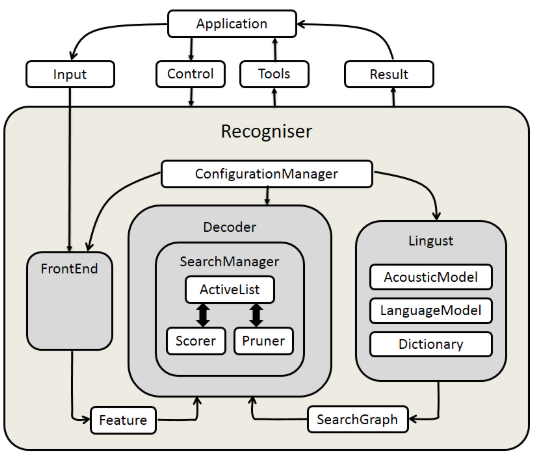
\includegraphics[width=9cm]{thesis/images/sphinx}\\
  \caption{CMU Sphinx4 recogniser system. The core modules: \texttt{FrontEnd}, \texttt{Decoder} and \texttt{Linguist} coloured in grey.}\label{fig_c3_sphinx}
\end{figure}
In the CMU Sphinx realisation, the \texttt{FrontEnd} module implements feature extraction.  The \texttt{Linguist} module implements the acoustic modelling and the language model component. Finally, the \texttt{Decoder} module implements a decoder.  The \texttt{ConfigurationManager} class is used to determine the behaviour of the recogniser by specifying the parameters of the other modules.   

From this implementation, the \texttt{FrontEnd} processor is the signal processing unit of Sphinx-4 parameterising signals using various implementations into a final sequence of \texttt{Features}.  The \texttt{Linguist} is in charge of language and pronunciation modelling.  This includes phonetic information from the \texttt{Dictionary} and structural information from one or more sets of \texttt{LanguageModel}s and \texttt{AcousticModel}s.  The output of the \texttt{Linguist} is a \texttt{SearchGraph}.  The \texttt{Feature}'s output from the \texttt{FrontEnd} and the \texttt{SearchGraph} output from the \texttt{Linguist} become the input for the \texttt{SearchManager} in the \texttt{Decoder}.  The output of the decoder are \texttt{Results} objects.  At any time prior to or during the recognition process, the researcher can via his application application issue Controls  through the \texttt{ConfigurationManager} to each of the modules, and become a partner in the recognition process.  The following subsections summarise the submodules \citep{walker2004sphinx}.

\subsubsection{FrontEnd Module}
Being consistent with having a ``pluggable'' framework, CMU Sphinx4 has the ability that most of its components can be replaced and at run-time.  This flexibility allows various implementations of the comprising components of the recogniser.  Accordingly, the front end supports but is not limited to \acrfull{mfcc}, \acrfull{plp} and \acrfull{lpc} implementations.  In addition, comprising modules within the various implementations include support for various signal processing utilities such as Hamming Windows, \acrfull{dct}, Bark Frequency Warping, Mel Frequency Filtering, \acrfull{cmn} etc.  All the tasks therefore required by the feature extraction process are implemented in this module.

\subsubsection{Linguist}
The job of the \texttt{Linguist} is to model the higher order and lower order grammar content of the audio input.  This particular module caters for the acoustic model and the language model.  The  various \texttt{Linguist} implementations allow CMU Sphinx-4 to support different tasks such as traditional \acrfull{cfg}, \acrfull{fsgs}, finite-state transducers and small N-gram language models.  This module has three pluggable modules representing the \texttt{Dictionary}, \texttt{LanguageModel} and \texttt{AcousticModel}.  The \texttt{Dictionary} comprises the pronunciation of all the words to be used in the \texttt{Decoder}. Sphinx-4 Linguist provides primary support for the CMU Pronouncing Dictionary (Carnegie Mellon University, 2016). The \texttt{SearchGraph} produced by the Linguist is capable of sharing parameters such as Gaussian mixtures, transition matrices and mixture weights and Sphinx-4 provides a single Acoustic model supporting acoustic models generated by the Sphinx-3 trainer.  Depending on the memory architecture various implementations of the Linguist include the \texttt{FlatLinguist}, \texttt{DynamicFlatLinguist} and \texttt{LexTreeLinguist}.  These will either create the \texttt{SearchGraph} entirely in memory or on demand.  Finally, the \texttt{LanguageModel} supports a variety of formats such as \texttt{SimpleWorldListGramar} which as the name implies supports a simple word list.  The \texttt{JSGFGramar} is a BNF-style platform-independent realisation of the Java Speech API Grammar format. \texttt{LMGrammar} produces a bigram model. \texttt{FSTGrammar} supports finite-state transducer ARPA FST grammar format. The \texttt{SimpleNGramModel} support N-gram model and the \texttt{LargeTriGramModel} is suited to optimise memory storage.

\subsubsection{Decoder}
Provides a pluggable \texttt{SearchManager} to simplify decoding.  \texttt{Decoder} tells \texttt{SearchManager} to recognise a set of \texttt{Feature} frames. This creates a \texttt{Result} object that contains all the paths that have reached a final non-emitting state(i.e. Word endings).  Applications can modify the search space and Result object between steps, permitting the application to become a partner in the recognition process.  The \texttt{SearchManager} is not restricted on any particular implementation, examples include Frame synchronous Viterbi, Bushderby, A*, bi-directional and parallel searches.

Each \texttt{SearchManager} uses a token passing algorithm described by (Young, Russel & Thornton, 1989).  A sphinx-4 token is an object that is associated with a \texttt{SearchState} and contains the overall acoustic and language scores of the path at a given point, a reference to the \texttt{SearchState}, a reference to an input \texttt{Feature} frame, and other relevant information.

The \texttt{SearchManager} sub-framework generates \texttt{ActiveLists} from currently active tokens in the search trellis by pruning using a pluggable Pruner. These in turn can be modified by the application to perform both relative and absolute beam pruning.

The \texttt{SearchManager} sub-framework also communicates with the \texttt{Scorer}, a pluggable state probability estimation module that provides state output density values on demand.

\subsubsection{Other modules}
\texttt{ConfigurationManager} allows various module implementations to be combined in various ways.  Finally, we illustrate how the \texttt{ConfigurationManager} creates Automatic Speech Recognition (ASR) experiments using the CMU-sphinx4 objects described above in the sample program from \cite{Lamere03thecmu} 
\begin{lstlisting}[language=Java,basicstyle=\small]

package com.example;
import java.io.File;
import java.io.FileInputStream;
import java.io.InputStream;

import edu.cmu.sphinx.api.Configuration;
import edu.cmu.sphinx.api.SpeechResult;
import edu.cmu.sphinx.api.StreamSpeechRecognizer;

public class TranscriberDemo {                                  
    public static void main(String[] args) throws Exception {      
        Configuration configuration = new Configuration();
        configuration
        .setAcousticModelPath("resource:en-us");
        configuration
		  .setDictionaryPath("resource:cmudict-en-us.dict");
        configuration
        .setLanguageModelPath("resource:en-us.lm.bin");

        StreamSpeechRecognizer recognizer = new StreamSpeechRecognizer(
                configuration);
        InputStream stream = new FileInputStream(new File("test.wav"));

        recognizer.startRecognition(stream);
        SpeechResult result;
        while ((result = recognizer.getResult()) != null) {
            System.out.format("Hypothesis: %s\n", result.getHypothesis());
        }
        recognizer.stopRecognition();
    }
}
\end{lstlisting}
The above java code sample represents a user application.  We see three classes being imported. The \texttt{Configuration}, \texttt{SpeechResult}, and \texttt{StreamSpeechRecognizer} class.  The \texttt{Configuration} object holds resources for the acoustic model, language model and phonetic dictionary.  The \texttt{SpeechRecognizer} object has different implementations representing the source of the speech signal.  In the above sample the \texttt{StreamSpeechRecogniser} class is used to load the speech signal from a wave (.wav) file.  However other speech signal sources are available such as the \texttt{LiveSpeechRecogniser} which implements loading the speech sound signal from a microphone device if available.  In addition, \cite{walker2004sphinx} 4 asserts that the Sphinx-4 system provides additional tools and utilities that contain helper classes for computing recognition statistics such as Word Error Rate (WER), phoneme error rates (PER) etc.

\subsection{Kaldi}
CMU Sphinx provides an object-oriented approach to speech recognition. Kaldi \cite{povey2011kaldi} on the other hand is a highly modularised library written in C++. Kaldi is based on weighted finite state transducers (WFSTs) used for inference graphs and decoding. The Kaldi WFSTs utilises OpenFst, an open source library, at its core. Together with a collection of configuration scripts for building complete recognition systems, Kaldi supports modeling of a variety of speech model variations with vast support for linear and affine transforms of speech features of arbitrary phonetic-context sizes.  Kaldi is specifically suited for acoustic modeling with subspace Gaussian Mixture Models (SGMM) in addition to the standard Gaussian Mixture Models (GMMs).
\subsubsection{Architecture}
The component architecture of Kaldi is illustrated in the figure below.  Modules can be divided into those that utilise the linear algebra libraries and those that use OpenFST.  The decodable class forms the link between these two scopes.  The rest of the modules lower down the hierarchy are based on modules higher up hierarchy according to this divide.
\begin{figure}
\centering
  % Requires \usepackage{graphicx}
  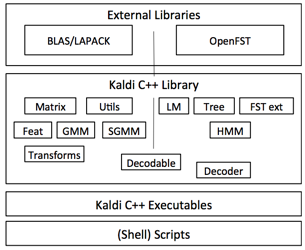
\includegraphics[width=9cm]{thesis/images/kaldi}\\
  \caption{ The Kaldi Architecture\citep{povey2011kaldi} has four layers.  At the deepest layer are the external libraries, followed by the C++ back-end library.  At the top: are the C++ executables called by shell scripts }\label{fig_c3_kaldi} 
\end{figure}
\subsubsection{Feature Extraction}
Kaldi supports various speech feature outputs including the standard \acrfull{mfcc}, \acrfull{plp}, \acrfull{vtln}, \acrfull{cmvn}, \acrfull{lda}, \acrfull{stc},\acrfull{mllt}, \acrfull{hlda}.  These systems are made complete with various configuration parameters for fine tuning their individual models.
\subsubsection{Acoustic Modelling}
Full co-variance as well as diagonal co-variance GMM modelling is implemented in Kaldi. Efficient log-likelihoods are computed using simple dot products of mean times in-variance and in-variance co-variance.  The \texttt{DiagGmm} class is responsible for storing co-variances of Gaussian densities. The Acoustic Modelling (AM) class represented by the \texttt{AMDiagGmm} class comprise a set of \texttt{DiagGmm} objects.  These objects which represent Gaussian Mixture Models (GMMs) are in turn represented Probability Density Function (PDF) indices which are then mapped to \acrfull{hmm} states. There are classes to represent HMM topology as well as the overarching topology representing transition modelling. These two sets of classes provide information required for developing decoding graphs.  Rather than using the conventional approach for HMM modelling using hand-made decision tree for left and right phones in a mono-phone model, tree-clustering algorithms automatically generate the decision tree.

\subsubsection{Language Modelling and Decoding Graphs}
Using the \acrfull{fst} back in addition to third party language modelling software, Kaldi is able infer sentence estimations using n-gram language models. During decoding, transition-ids are created and attached to corresponding pdf-IDs as a result of tied-state nature of phones where different phones are allowed to have share the same distribution.  The transition-id therefore encapsulates the shared pdf-ID and the arc (transition) of phone-specific topology. This way transitions are fine-grained without adding complexity to the decoding graph

Core decoding algorithms are implemented using C++ classes one per decoder.  Decoders implement an interface which accepts an acoustic model score for a particular input-symbol and frame.  While single-pass decoding is achieved through C++ classes, multi-pass decoding is realised using the supporting configuration scripts.

\subsection{Mozilla DeepSpeech}\label{sec_c3_moz}
The DeepSpeech speech-to-text engine is an ASR speech model and model generator built by Mozilla is based on Baidu's Deep Speech research paper \citep{hannun2014deep}.  The system comes in two forms;  an installable speech-to-text engine based on the English language and the model trainer. These components were created and run effectively on Unix based systems and to a limited extent on Microsoft Windows systems.  Various options for installing the speech to text engine includes either command line based or as an application programming interface (API) using python or NodeJS.  In addition, the speech-to-text (STT) engine API also supports bindings for the Rust language, GoLang and GStreamer.  This thesis however, did not rely on the STT engine nor API, but rather on the model trainer which was adapted in this research for scattering transform feature-based end-to-end speech recognition.

Runtime library dependencies of both the STT engine and the model trainer include libsox, 2 for sound processing of audio; libstdc++6, libgomp1 and libpthread are used to compile the Connectionist Temporal Classification (CTC) decoder implementation which incorporates the KenLM trained language model \citep{Heafield-estimate}.
\subsubsection{Graphics Processor Unit (GPU)-Enabled Speech Model Training}
The model trainer of the Mozilla DeepSpeech platform is facilitated by the ability to train models on a highly parallel processing Graphics Processing Unit (GPU).  This enables model training-time speed-ups over traditional CPU machines.  The Mozilla DeepSpeech platform recommends Nvidia Graphics 10 series processor with a system requirement of 8GB of Random Access Memory (RAM). In section \ref{sec_c3_tf} we introduce TensorFlow python library.  Mozilla DeepSpeech platform is able to utilise the GPU using the Nvidia GPU library, CUDA.  This is achieved through the python TensorFlow library created by Google as discussed in section \ref{sec_c3_tf}.
\subsubsection{Common Voice training}
The speech corpus used for training in this research was obtained from the Mozilla Common Voice Initiative speech corpora.  This consists of over 250 hours of speech data that is subdivided into test, development and training data sets.  In addition, the data was subdivided into clean data, that is, clean audio recording with accurate translation and a small subset containing skewed data, that is, audio recording which was either noisy or lacking accurate transcriptions.  The skewed data subset consisted 15-25\% of the training corpus and was incorporated so that the neural network speech model could simulate and learn real world noisy audio speech-to-text translation.  The Mozilla DeepSpeech model trainer provided bash scripts for importing the Common Voice speech corpora as well as converting the files into the appropriate formats and provision of mapping files for the model trainer.
\subsubsection{Mozilla DeepSpeech model parameters}
The model trainer consists of a root python script ``DeepSpeech.py'' with various calls to other python scripts responsible for things like audio processing, distributed training, GPU configuration, training coordination.  Other accessory bash scripts also present are responsible for downloading and training for different kinds of speech corpora including Mozilla Common Voice\citep{ardila2019common} and the Wall Street Journal (WSJ)\citep{paul1992design}.  These sets of scripts are referred to as speech corpus importers. 

In order to supply the model trainer with a set of hyper parameters for tuning various aspects of the Mozilla DeepSpeech platform, the following categories arguments passed to the root script ensue:
\begin{itemize}
    \item Geometry - Defines the number of neurons in the hidden layers of the neural network.
    \item Cluster configuration - Parameters responsible for distributed training of the speech model across various nodes.
    \item Global constants - These include all other parameters to gain fine control of the training process.  These parameters include how much of the training corpus will be used and which subset should be included; early stopping for pre-trained models that have already been trained to saturation, that is to a stopping condition; the dropout rate for neural network regularisation.  This is a strategy to overcome over-fitting where instead of learning inference features the data, the neural network memorizes the training data.
    \item Global constants - These include all other parameters to gain fine control of the training process.  These parameters include how much of the training corpus will be used and which subset should be included; early stopping for pre-trained models that have already been trained to saturation, that is to a stopping condition; the dropout rate for neural network regularisation.  This is a strategy to overcome over-fitting where instead of learning inference features the data, the neural network memorizes the training data.
    \item Adam optimiser - parameters for the Adam optimiser
    \item Batching - set the number of batches during training.
    \item Weight Initialisation - standard deviation coefficients for initialising weights.
    \item Checkpointing - this includes the number of seconds before saving the current model parameter values to the disk.  This enables resumption of training in instances where the training was interrupted. For training to resume successfully, the resuming training geometry parameter must be exactly the same as the interrupted geometry training parameter.
    \item Exporting - Includes parameters for saving a saturated model for inference.
    \item Reporting - Includes options for setting the log-level however reports are only sent to the standard console output.
    \item Decoder - These parameters include the path to the alphabet symbols and that of the custom CTC decoder used during decoding of the neural network output.
    \item Inference - It is possible to use a model trainer to either perform a one-shot inference or resume training from an already exported model. The parameters used for inference are responsible for performing these stated tasks.
\end{itemize}

In addition to the above configuration there are other accessory scripts that can be used for TensorFlow specific tasks such as conversion of the output model graph to several exportable formats.

\subsection{Matlab and ScatNet toolbox}
In this research, feature processing of audio files to obtain their deep scattering transforms was achieved using a MATLAB toolbox known as ScatNet \citep{anden2014scatnet}.  The ScatNet toolbox in general analyses time-series sampled analog signals and has been used successfully for music genre classification, texture and image classification \citep{anden2011multiscale,sifre2013rotation,sifre2014rigid}.  In particular, the scattering transforms produced are signal processing layers of increasing width where each layer constitutes the convolution of a linear filter bank wavelet operator (Wop) with a non linear complex modulus.  
\begin{equation}
    ||\text{complex signal}|\star \mathbf{Wop}|\star(\text{low-pass filter}) \label{eqn_c3_scat00}
\end{equation}

It is the scattering transforms of the audio files that were fed into the DeepSpeech model trainer discussed in Section \ref{sec_c3_moz}.  The architecture of a scattering networks resembles a deep convolutional network in the sense that each subsequent layer is a mapping of all possible paths from the previous layer.

ScatNet provides default options for most of the parameters that require tuning in order to derive the scattering coefficients for an input signal.  In particular, for audio signals, the most important hyper-parameters set by the library is the number of scattering layers that captures the entire audio spectrum which is set at 2.  In addition to this default, the only other parameter to set is the window period of the signal to be analysed per time.  A suitable value for the window can be derived from the sampling rate of the input signal.  The toolbox function \texttt{S=scat(x,Wop)} takes a an input signal, \texttt{x},  and an array of linear wavelet operators, \texttt{Wop}, in order to compute the scattering coefficients of the input signal.   The resulting network, \texttt{S} is a cell array whose length $M+1$ is equivalent to that of the linear filter operator.  

\subsubsection{Wavelet Factories}\label{sec_c3_scat00} 
By providing optimal defaults for linear operators, ScatNet provides wavelet factories especially suited for efficient signal processing of images and sounds.  Therefore, linear wavelet operators are built in a single command function through built-in “factories”, which perform wavelet analysis tasks.

Further, the maximum number of wavelets $J$ is automatically derived from the sampling from the sampling period $T$.  The filter banks are formed by dilating the mother wavelet ($\psi$) by the dyadic factor ($2^{1/Q}$).  In the Fourier domain this is expressed as
\begin{equation}
     \hat\psi_j(\omega) = \hat\psi(2^{j/Q}\omega)
     \label{eqn_c3_scat01}
\end{equation}
For audio application, to ensure optimized frequency coverage without frequency-redundancy or overlapping, the mother wavelet $(\psi)$ is chosen so that  $(Q_1 = 8)$ and $(Q_2 = 1)$ by default. This also means that the first order filter will be of a higher frequency resolution when compared to the second order filter. 
\subsubsection{Filter banks}\label{sec_c3_scat01}
In order to visualise the filters being used by the wavelet operations and referring to Sections (\ref{sec_c5_wproof} and \ref{sec_c7_wparams}) where it is shown that the first and second order scattering coefficients are respectively defined by the following forms
\begin{equation}
    S_1x(t,j_1) = |x\star\psi_{j_1}|\star\phi(t)
    \label{eqn_c3_scat02}
\end{equation}
\begin{equation}
    S_2x(t,j_1,j_2) = ||x\star\psi_{j_1}|\star\psi_{j_2}|\star\phi(t) \label{eqn_c3_scat03}
\end{equation}
where $(\psi_{j})$ are band-pass filters and $(\phi)$ is  a low-pass filter.

Furthermore, the wavelet transform operators(Wop) created by the wavelet\_factory\_1d function are only function handles and do not have any data in themselves. A second return value may be retrieved from the wavelet factory which contains the set of filters returned as a cell array by the wavelet factory.
\begin{verbatim}
    [Wop,filters] = wavelet_factory_1d(N, filt_opt);
\end{verbatim}

The filters return argument has a similar structure to the scattering network where each element in the cell array corresponds to the layer order in the scatter network hierarchy. Moreover, similar to the the scatter network, the filters cell array hierarchy has $M+1$ elements, where only $M$ elements are utilised and no filters exist at $M=0$. The non-zero coefficients of the band pass filters expressed in the Fourier domain, are held in \texttt{filters{m}.psi.filter} field. When plotting these filters, they are first padded with zeros to the length of \texttt{N} which is the entire spectrum.  Below is the sample plot made against default filters obtained by the \texttt{wavelet\_factory\_1d} filter.

The script below calculates filter banks at orders $(M = 1)$ and $(M = 2)$.  The resulting plot is displayed in Figure \ref{fig_c3_wplot}.

\begin{lstlisting}[language=Matlab]
figure;
for m = 1:2
    subplot(1,2,m);
    hold on;
    for k = 1:length(filters{m}.psi.filter)
        plot(realize_filter(filters{m}.psi.filter{k}, N));
    end
    hold off;
    ylim([0 1.5]);
    xlim([1 5*N/8]);
end
\end{lstlisting}

\begin{figure}
\centering
  % Requires \usepackage{graphicx}
  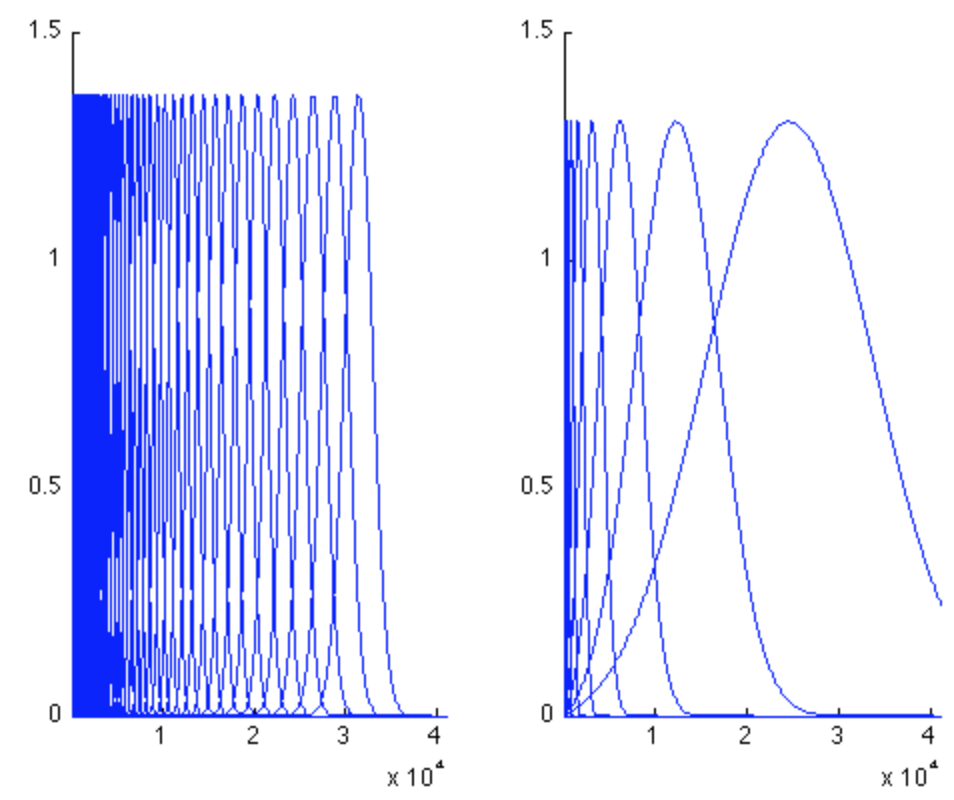
\includegraphics[width=9cm]{thesis/images/wfplot}\\
  \caption{Scatter transform wavelet filter plots of various dilations of $J$}\label{fig_c3_wplot}
\end{figure}

\subsubsection{Using the Matlab API}\label{sec_c3_scat02}
In the previous sections it was seen how the ScatNet toolbox calculates scatter coefficients based on wavelet theory.  In this section, the scattering spectrum of an audio signal is implemented using only three command calls to ScatNet library.

The three steps taken in this section are as follows.  First load the audio file and set the properties of the audio file required for audio processing of the signal within ScatNet.  Note that to do this the sampling rate of the input signal is required. Here, a clip of Handel’s Messiah, implemented in Matlab as a function is loaded into a “y” variable by default with the “load handel” command.

Given that the sampling rate of the loaded clip is , the parameters set are 
\begin{enumerate}
    \item N - the number of samples in the signal, and  
    \item T - the window size.  Here, T is set to 4096 which corresponds to about half a second.
\end{enumerate}
\begin{verbatim}
    load handel;	% loads the signal into y
    N = length(y);
    T = 2^12;   	% length of the averaging window
\end{verbatim}

The second step is to create the filter operators for which the type of filter signal length, and the window length are passed in as parameters.  It has been shown in the preceding sections that two layers are sufficient to capture energy contained in an audio signal and by default the quality factors of the two layers are $(Q_1 = 8)$ and $(Q_2 = 1)$. These default\_filter\_options are automatically integrated with the 'audio', filter type option.
\begin{verbatim}
    filt_opt = default_filter_options('audio', T);
    Wop = wavelet_factory_1d(N, filt_opt);
\end{verbatim}
Note that the wavelet\_factory\_ functions is an intensive operations because many filters are being built at once  in batch processing of signals discussed in Section \ref{sec_c3_sbatch}, we therefore only perform this as part of the initialisation and the returned wavelet operators (Wop) can be reused without having to recreate them.

Having all the parameters required, in the third and final step , call the scattering transform of y generic function scat, to derive the scatter coefficients.
\begin{verbatim}
    S = scat(y, Wop);
\end{verbatim}

\subsubsection{Scatter Feature Enhancements and Batch Processing}\label{sec_c3_sbatch}
Having obtained the scatter coefficients, further feature enhancement is achieved by taking the log of the normalised coefficients.  This can be visualised using the  built-in scattergram function which produces a translation-invariant, second-order, spectrogram-like visualization of the  scattering transform a one-dimensional audio signal. 

In the code snippet below, \texttt{j1} is the second-order coefficients arbitrarily chosen to equal \texttt{23}.  The first parameter to scattergram are the first-order coefficients and the second wildcard [] parameters gathers all paths from the first order.  
\begin{verbatim}
    j1 = 23;
    scattergram(S{2},[],S{3},j1);
\end{verbatim}

\begin{figure}
\centering
  % Requires \usepackage{graphicx}
  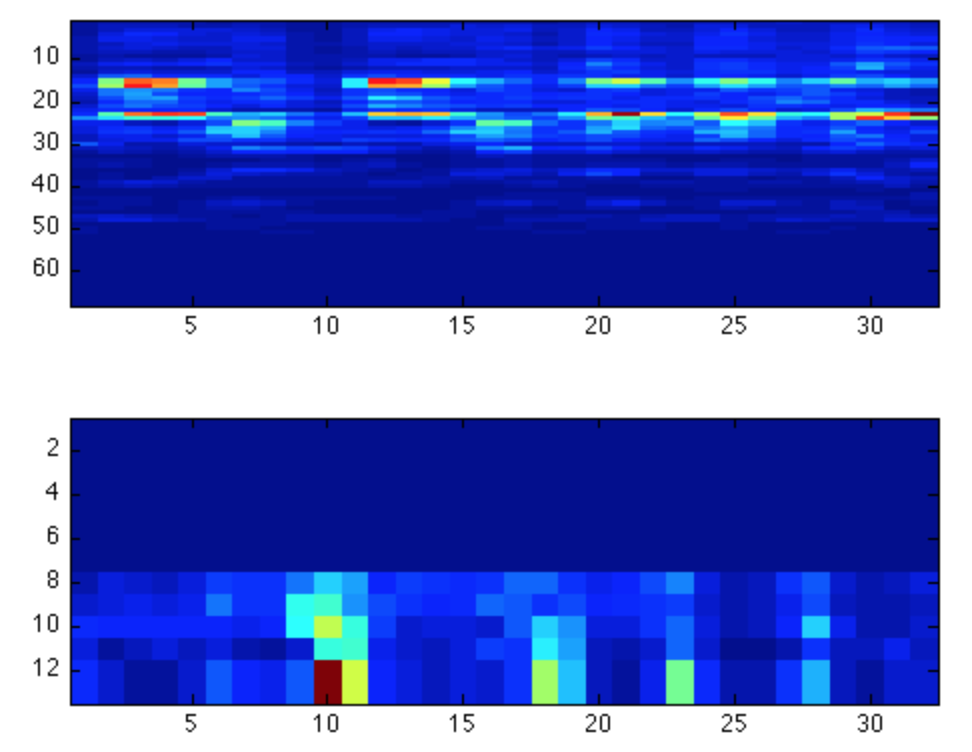
\includegraphics[width=9cm]{thesis/images/wscat0}\\
  \caption{Unnormalised scattergram}\label{fig_c3_sgram00}
\end{figure}

The following functions in the code snippet below are applied to realise the log of the normalised scattergram.
\begin{verbatim}
    S = renorm_scat(S);
    S = log_scat(S);
    scattergram(S{2},[],S{3},j1);
\end{verbatim}

\begin{figure}
\centering
  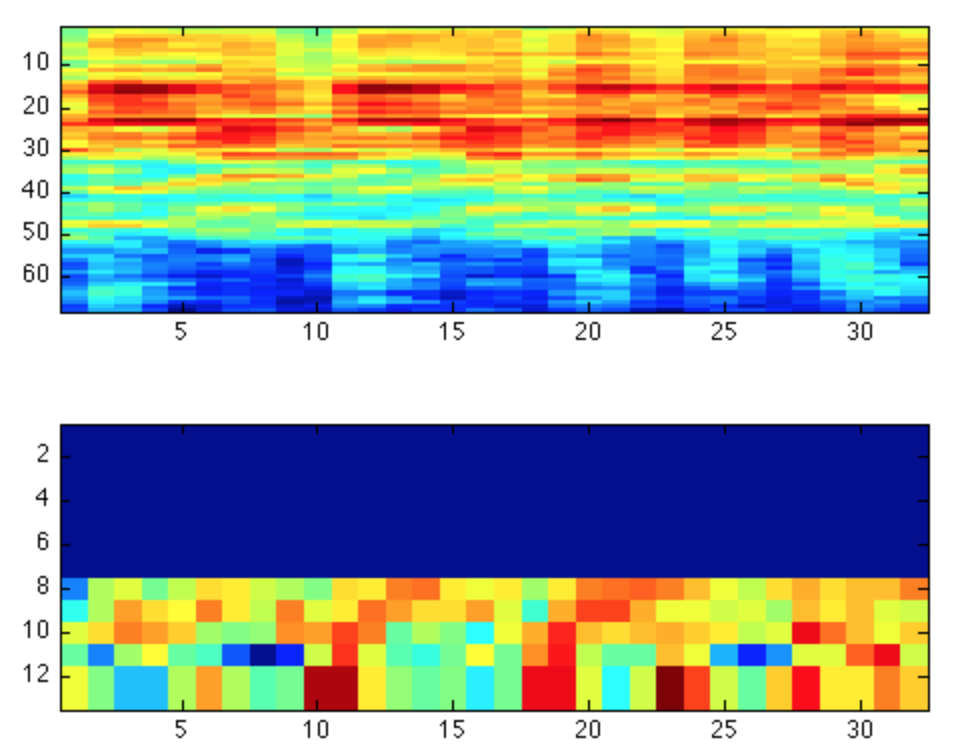
\includegraphics[width=9cm]{thesis/images/wscat1}\\
  \caption{Log normalised scattergram}\label{fig_c3_sgram01}
\end{figure}

With the corresponding scattergram illustrated in figure \ref{fig_c3_sgram01}.

Finally, to utilise the scattering coefficients as features for classification tasks, we extract the vector form using \texttt{format\_scat} function.
\begin{verbatim}
    [S_table, meta] = format_scat(S);
\end{verbatim}

The \texttt{S\_table} is a P-by-N table, where \texttt{P} is the flattened total of all the scattering combined coefficients within each layer of the \acrfull{dsn} and \texttt{N} is the number of time points. The network is now feature ready for classification tasks using an affine space classifier.

For batch processing ScatNet provides a database feature which can accept a collection of input vectors rather than a single input signal.  The following commands show ScatNet commands for performing batch processing on the GTZAN dataset used for musical genre classification

First, specify the path to the audio target.
\begin{verbatim}
    src = gtzan_src('/path/to/dataset');
\end{verbatim}

Next all the defaults for ScatNet analysis and processing are set as explained in the previous Sections \ref{sec_c3_scat00},\ref{sec_c3_scat01} and \ref{sec_c3_scat02} above.
\begin{verbatim}
    N = 5*2^17;
    T = 8192;
    filt_opt.Q = [8 1];
    filt_opt.J = T_to_J(T, filt_opt);
    scat_opt.M = 2;
    Wop = wavelet_factory_1d(N, filt_opt, scat_opt);
    feature_fun = @(x)(format_scat( ...
    log_scat(renorm_scat(scat(x, Wop)))));
\end{verbatim}

It is possible to optimise the training by sub-sampling each signal.  The feature\_sampling option is used to specify sub-sampling.
\begin{verbatim}
    database_options.feature_sampling = 8;
\end{verbatim}


Finally, a call is made to \texttt{prepare\_database} function to compute all the scatter network features of the \texttt{src} database.
\begin{verbatim}
    database = prepare_database(src, feature_fun, database_options);
\end{verbatim}

In this research, further speed up was achieved by utilising Matlab’s parallel processing on the for loop (see Appendix III) thus bypassing the batch processing utility of ScatNet.

\subsection{TensorFlow}\label{sec_c3_tf}
TensorFlow is a state-of-the-art high performance library by Google for Deep learning.  Deep learning is a branch of artificial intelligence which acquires learning from deep neural network architectures.  The paragraphs and subsections that follow under this topic give an overview of the TensorFlow library as outlined by the following authors \cite{goldsborough2016tour,abadi2016tensorflow} and \cite{abadi2017computational}.

Deep learning has significantly advanced in various application domains and by far out-performed traditional approaches.  TensorFlow offers researchers and enthusiasts an open source software library for use in defining, training and deploying deep learning models.

TensorFlow works by defining data flow graphs with mutable state.  A data flow graph represent complex functional node and edge architectures, where each node represents an operator instance applied to input values which constitutes the edges. The operators are implemented by abstract kernels for particular types of interchangeable devices (such as CPUs and GPUs)\citep{abadi2017computational}.

There are three main concepts at TensorFlow's core.  These concepts are tensors, operations and mutability.  Tensors are arrays of arbitrary dimensions where the underlying data type is either specified or inferred at graph-construction time. Operations process data and constitute nodes within the compute graph. Basic operations invariably are mathematical functions such as vector dot products.  However, some of the operations indeed may be associated with a read or state update. Such tensor which permit run-time updates in TensorFlow are referred to as variables.  Finally, there may be edges for communicating and constrain the order of execution. These structures invariably affect the observable graph semantics and may also affect the computation performance. 

Once a TensorFlow program constructs a graph using a client interface such the Python API, the TensorFlow program can send messages to the graph, by “feeding” it inputs and “fetching” outputs from it. TensorFlow then propagates the input values through the execution graph performing  operations called by the client code, until all nodes instructed to run returned with their outputs. 

Data dependencies and control edges, dictate the order of execution. Often, a graph is executed severally and tensors declared as placeholders or constants are used once. However, variable tensors have mutable state which allow persistence across multiple executions. The parameters of the model stored in variables are usually updated as part of running the graph.

\subsubsection{Programming Model}
In this section examples of execution data flow graphs are given; and in the following sections we highlight the other major special features of TensorFlow including automatic differentiation and back-prop algorithm implementation, control flow, check pointing, programming interface, sample implementation and graph visualisation.

In a TensorFlow computational data flow graph, vertices or nodes of the directed graph represent operations, while edges signify flow of data between these vertices or operations. Thus labels on nodes are representative of the actions taken at that node.  Similarly, labels representing values flow in the direction of the edges. The inputs to a labeled operation are therefore the labels which have edges directed towards the operation. A computation or data flow graph is illustrated in Figure \ref{fig_c3_tfg}. 
\begin{figure}
\centering
  % Requires \usepackage{graphicx}
  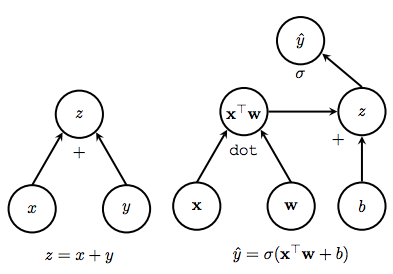
\includegraphics[width=9cm]{thesis/images/tfgraph}\\
  \caption{Sample TensorFlow computation graphs\citep{goldsborough2016tour} showing a simple addition operation on the left and a more involved sequence on the right comprising a dot operation followed by an addition and then a sigmoid operation}\label{fig_c3_tfg}
\end{figure}

The left graph displays a basic compute graph consisting of an addition operator having two input variables $x$ and $y$.  The result, $z$ is the output of the $+$ operation.  The right graph gives an example logistic regression function. $\hat{y}$ is the final output of the function for some sample vector $\mathbf{x}$, weight vector $\mathbf{w}$ and scalar bias $b$.  As shown in the graph, $\hat{y}$ is the output of the sigmoid or logistic function $\sigma$

\subsubsection{Backprop nodes}
The Backprop algorithm \cite{Goodfellow-et-al-2016} is an efficient method to compute error values for weights within a multilayer or deep neural network.  The algorithm is summarised as follows.  Assuming a neural network with two hidden layers. The two layers within the network respectively have output functions $f(x;w)$ and $g(x;w)$ such that $f(x;w)=f_x(w)$ and $g(x;w)=g_x(w)$.  Where $x$ is the input from the previous layer or from the input layer and  are the weights.  The error function , is an implicit function of all the previous layers.  In the case of the 2-layer network $e=(f_x \circ g_x)(w)=f_x(g_x(w))$.  The back prop algorithm uses the chain rule to correctly assign appropriate updates to each weight at every layer within the network.  The updates which are the gradient or the error function with respect to the weights are $de_x/dw$. The backprop algorithm therefore uses the formula $[f_x(g_x(w))]'=f'_x(g_x(w))\cdot g'x(w)$ as it traverses the graph in reverse to compute the updates. 
\begin{figure}
\centering
  % Requires \usepackage{graphicx}
  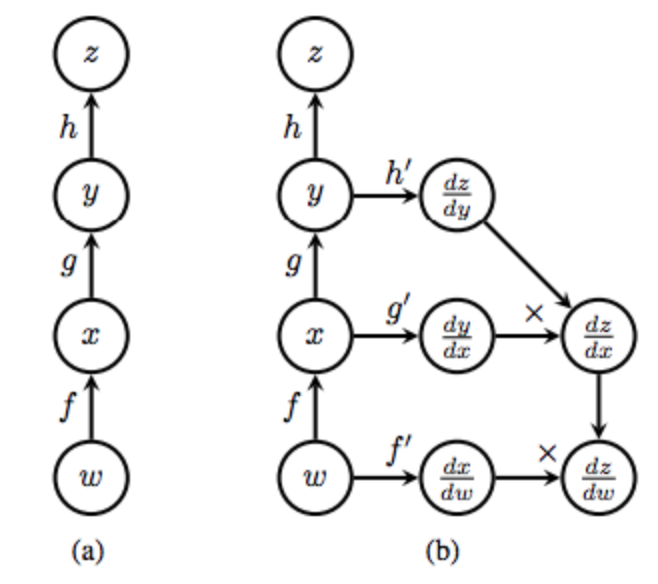
\includegraphics[width=9cm]{thesis/images/bprop}\\
  \caption{Tensorflow graph with backprop nodes \citep{goldsborough2016tour}.  The forward propagation is on the left (a) and; the Forward propagation with back propagation (b) is on the right}\label{fig_c3_bprop}
\end{figure}

Figure \ref{fig_c3_bprop} illustrates how tensor implements backprop by adding two extra nodes at the appropriate layers within the network to satisfy the chain rule.  For each operation encountered, there is a corresponding gradient function that reverses the output as a function of the inputs.  The output of this gradient function can then be propagated backwards to a previous operation which would represent a previous layer within a neural network.  The gradient function propagated to the previous layer is then used to complete the parameters of the chain rule by multiplying with that previous layer’s gradient.  This output is ready to be propagated down the network to the subsequent layer to perform a similar function.  This process continues until all the weights within the network have appropriate update values.

\subsubsection{Control flow}
TensorFlow also supports control-flow operations.  For this reason TensorFlow is not a directed acyclic graph (DAG) but can support cyclic structures. If the number of loops required by the computation graph is known at graph construction.  It is easy to maintain a DAG structure simply by unrolling the number of loops specified.  However, this is not always the case.  There are instances in which a variable number of loops is required at runtime.  Hence, the computation graph becomes increasingly complex.  This is particularly the case for back gradient descent and back propagation of errors (see section \ref{sec_c3_tfw} for a  walk through).  The process of stepping back through a loop in reverse to compute gradients is known as back-propagation through time \citep{al2016theano}.

\subsubsection{Checkpoints}
One can add Save a node to a compute graph, connecting them to variables whose tensors can then be serialized. At another instance one may connect the same variable to a Restore operation. This operation deserializes the stored tensor at another point within the execution graph. This is especially useful over long periods of training to keep track of the model’s variable parameters. These elements form part of distributed TensorFlow's fault tolerance ecosystem.

\subsubsection{Programming Interface}
TensorFlow implementation provides two developer interfaces which include the Python interface and the C++ interface.  While the python interface offers a rich feature set for creation and execution of computation graphs, the C++ interface is primarily a back end implementation with a much more limited API primarily used for executing graphs built with Python and serialised to Google’s protocol buffer.

It is worth noting that unlike PyTorch \citep{ketkar2017introduction}, the Python API handshakes very well with NumPy\citep{numpy} numeric and scientific open source programming library. As such, TensorFlow tensors can be naturally substituted with NumPy ndarrays without any need for type-conversion seen in PyTorch tensors.

\subsubsection{Tensorflow client model walk through}\label{sec_c3_tfw}
In this section, a sample client tensorflow model is examined. The model consists of a simple multi-layer perceptron (MLP) with one input and one output layer to classify hand-writtin digits in the MNIST\citep{krizhevsky2012imagenet} dataset.   In this dataset, the examples are small images $28 \times 28$ pixels depicting handwritten digits from $0$ to $9$.  The examples form a matrix having the shape $\mathbf{X}\in\mathbb{R}^{n\times 784}$ where  represents the number of images, and 784 represents the flattened 28 x 28 pixel image.  The client code performs an affine transform operation, $\mathbf{X\cdot W+b}$, where $\mathbf{W}$ is the matrix of weights $\in \mathbb{R}^{784 \times 10}$, and $\mathbf{b}$ is a vector of biases  $\in R^{10}$.  The result of the affine transform operator is the matrix $\mathbf{Y}\in \mathbb{R}^{n\times 10}$. The resulting non-probabilistic logits gives an unnormalised distribution of digits.In order to obtain the valid probability distribution $Pr[x=i]$ where $x$-th example is classified as the digit $i$, the soft-max method is utilised. 
\begin{equation}
softmax(\mathbf{x})_i=\frac{\exp(\mathbf{x}_i)}{\Sigma_j\exp(\mathbf{x}_j)}\label{eqn_c3_smax00}
\end{equation} 

Error loss values are then computed using an objective function and the model’s current training parameters $\mathbf{W}$ and .  This is obtained from the cross entropy calculation given by
\begin{equation}
    H(\mathbf{L,Y})_i=−\Sigma_j\mathbf{L}_{i,j}\cdot\log(\mathbf{Y}_{i,j})
\end{equation}

Where $\mathbf{Y}=softmax(\mathbf{x})$ and $\mathbf{L}$ are the correct one-hot-encoded labels.  More precisely, the batch-mean loss over all inputs $\mathbf{x}$.


Next, the \acrfull{sgd} is run to update the weights of our model.  A TensorFlow class is provided and will be initialised with a learning rate.  The minimise function of this class takes the loss tensor as parameter used for minimisation.

The operations run repeatedly within a \texttt{tf.Session} context manager. Refer to Appendix IV for the complete code listing.

\subsubsection{Visualisation}
TensorFlow interface offers the option of visualising computation graphs. Complex topologies consisting of various sub-layers can be presented in a lucid form, offering the user a congruent, organised picture of exactly how data is consumed in a compute graph. Sub-graphs may be grouped into visual blocks and referred to in name scopes.  For example a single neural network layer may take up such a named scope. The name scopes are then interactively expanded on to give the detailed group visualisation.

Two types of metrics are obtainable from the TensorBoard. These are summary operations, when attached as nodes in the graph, permit the user to monitor individual tensor values over time.   The first is the scalar summaries which capture tensor values and can be sampled at certain points within training epochs. One can now, for example, observe the trend of the accuracy loss of the training model over time.

The other summary operation offers the user the ability to track distributions, such as final soft-max densities or the distribution of neural network weights. 

Lastly, sample images can be visualised on the TensorBoard graph. This way kernel filters of a convolutional neural network can also be visualised.  In addition to all of these, one can perform zooming and panning actions directly on TensorBoard's web interface including expansion and collapsing of individual name scopes

\subsection{Choregraphe}
The Choregraphe software tool is a high-level language used for programming of Nao humanoid robots.  This is built on top of the Naoqi/Gentoo Unix/Robot Operating System(ROS) \citep{pot2009choregraphe}.  Speech recognition and processing modules of the Choregraphe tool were explored and expanded at the initial stages of the research.  However the Choregraphe software tool for the Nao robot was found to be unsuitable in speech recognition at the level of research that aligned with the research objectives and therefore was not utilised in this work.

\subsection{Alisa}\label{sec_c3_alisa}
Alisa tool is a lightly supervised sentence segmentation tool based on Voice Activity Detection (VAD) algorithms \citep{stan2016alisa}.  It is so-called "lightly supervised" because it requires small amounts of training data.  Generally the tool was asserted to be optimised for sentence segmentation and offered assistance in the creation of new speech corpora in a language-independent fashion. 

The Alisa tool researchers deploy a two-step method for aligning speech, and claim performance up to 70\% imperfect transcriptions often found in online resources can be successfully aligned with a word error rate of less than 0.5\%.  This tool is therefore said to be suitable for development multilingual and under-resourced language aligned speech-corpora.

The motivation behind Alisa was to reduce the time and effort used to gather large amounts of quality data as well as actively eliminate the domain knowledge required to phonetically transcribe speech data.  In addition, and as a bonus to achieving the first objective, is the ability to migrate speech technology fairly seamlessly from one language to another and therefore realise the rather tedious task of automatic transcription of a new language.

\subsubsection{Alisa Architecture}
The goal of automatic transcription of new language with low resource constraint is particularly valuable to this research and as such, it would be relevant to review the enhancements introduced to Alisa.  The two step-method consists of a GMM-based sentence level segmenter and also an iterative grapheme acoustic model used for alignment.  The sentence level GMM-based speech segmenter is used to automatically segment speech into utterances which as discussed earlier forms the basic unit of processing within any ASR system.  This attempts to relieve the researcher off the manual process of segmenting the continuous audio file manually. This process included a GMM-based voice activity detector trained from about 10 minutes of manually labeled data. The second step grapheme based acoustic model is supplemented with a highly restricted word network they referred to as a skip network.  Together an iterative acoustic modelling training procedure is formulated.  The method described required the initial training data and a minimal labelling procedure that involved simple letter to sound rules and inter-sentence silence segments to provide an orthographic transcript of the initial 10 minute recording data.  Therefore, this process is resource-effective because non-experts can also provide this data.  The actual alignment process made use of a grapheme level Viterbi decoder to drive the iteratively self-trained grapheme models.  The model architecture is shown in the figure below.
\begin{figure}
\centering
  % Requires \usepackage{graphicx}
  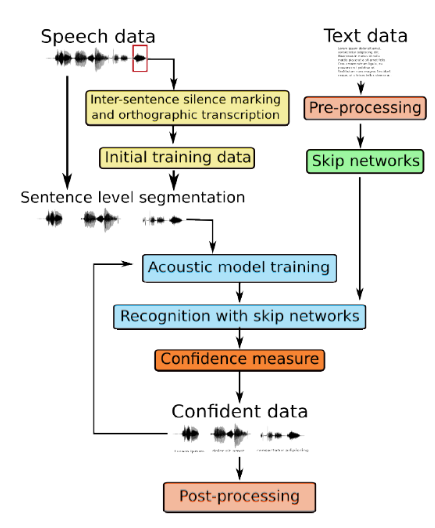
\includegraphics[width=9cm]{thesis/images/alisa}\\
  \caption{Alisa iterative architecture \citep{stan2016alisa} involving acoustic model, skip-network recognition and confidence level determination}\label{fig_c3_alisa00}
\end{figure}

Figure \ref{fig_c3_alisa00} shows a block diagram of the steps involved in the alignment.  The method can be applied to any language with an alphabetic writing system, given the availability of speech resource and its corresponding approximate script.

There is an option of using a grapheme based acoustic model. This however increases the margin for error.  Several steps were introduced in the Alisa tool to minimise this error margin. The chief being the introduction of a tri-grapheme acoustic model which is modeled after using context dependent triphones in traditional acoustic modelling.  Other techniques deployed to crash the error margin include the use of discriminative training with the Maximum Mutual Information (MMI) criterion \citep{schluter2001model} and methods described in \citep{novotney2009analysis}. It was observed that Alisa provided good alignment but was not fully featured. For instance it had no way of adding insertions and substitutions in the audio data not provided in the transcription.  Finally, Alisa was found to be restricted to only languages that can utilise the English alphabet.

\section{Pilot Studies}
The experiments in the following sections describe initial experiments based on the initial study of a language learning companion before the research was narrowed down to a low resource speech recognition.  These preliminary experiments in addition to a preliminary Language Learning Survey helped to narrow down the Research to the specific speech processing task of Low Resource Automatic Speech Recognition (LR-ASR).

The following sections describe analysis of raw wave-forms using auto-correlation signal processing in Matlab and experiments made with the Nao robot speech processing engine and experiments with speech recognition toolkit and speech processing tasks.  These tasks include digit recognition systems using CMUSphinx and Kaldi speech recognition toolkits and speech alignment tasks using the Alisa tool.

\subsection{Auto-correlation Experiments}\label{sec_c3_corr}
Preliminary experiments were carried out on raw speech signals in an attempt to quickly segment individual phonemes based on a basic threshold algorithm.  Further experiments designed an auto-correlation algorithm to attempt to discover a phoneme alphabet in a particular data set in a semi-supervised fashion.
 
\textcolor{blue}{This method had the goal of simulating posterior distributions of phonemes from auto-correlation estimates.  This presents an unnormalised posterior distribution measurement of phoneme segments over the entire signal.  Note that this was a pilot study, and as such, the data used as a single 3-second audio recording made by the researcher, as a demonstration of an alternative method to estimate phoneme distribution.  This experiment was designed for the purpose of exposure to Matlab audio processing toolbox. Furthermore, this research made use of more advanced correlation techniques in wavelets, in addition to the fact that the end-to-end method is able to make classification on a character and word-level.  There was therefore no need in performing all the design steps which would have included Segmentation, auto-correlation and then \acrfull{gmm} estimation.  The first two steps of segmentation and auto-correlation which was done for the single audio file is specified in the paragraphs below.}

The correlation theory is based on the idea that when a signals is superimposed on itself in a time-shifted manner, the convolution over itself is highest when the two signals have zero time lag that is, perfectly overlapped in sync and the better the overlapping the higher the value of the correlation and the lesser the signals are matched they tend to cancel out each other and hence a very low value of the correlation.  The normalised auto-correlation value is obtained in \cite{picone1996fundamentals} from a signal $x(n)$ in the following equation:
\begin{equation}
    \Psi(i)=\frac{\sum_{n=0}^{N-1}x(n)x(n-i)}{\left(\sum_{n=0}^{N-1}x(n)^2\right)\left(\sum_{n=0}^{N-1}x(n-i)^2\right)}\label{c3eq_corr}
\end{equation}

\textcolor{blue}{Based on experimental procedure, estimated locations of similar wave-forms representing the segmented phonemes are calculated.  Although the procedure is subject to degrade due to signal channel distortion associated speech production, this exercise helped to further emphasise the need for robust signal distortion invariant speech features and pre-processing highlighted in the section \ref{sec_2_3_3_scat}.}

This two stage procedure performs segmentation of phonemes and then discovery of phoneme clusters using a statistical auto-correlation algorithm.  The process is described in the following sections.
\begin{figure}
\centering
  % Requires \usepackage{graphicx}
  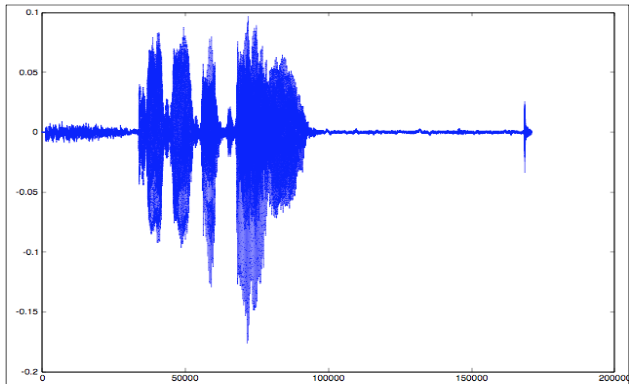
\includegraphics[width=9cm]{thesis/images/corr}\\
  \caption{Original waveform input from 3-second utterance for auto-correlation}\label{fig_c3_exp01}
\end{figure}

\subsubsection{Segmentation}
\textcolor{blue}{Generally, speech recognition preprocessing uses a fixed, overlapping window for segmentation. The segmentation algorithm designed for this experiment rather attempts to simulate and segment phoneme transitions using a natural phonetic  transition process between vowel (periodic signals) and consonants (non-periodic-noisy signals). Figure \ref{fig_c3_exp02} describes the various steps of the segmentation phase while Figure \ref{fig_c3_exp01} shows the original audio file. At the segmentation phase, we first of all adjust the scale of the original raw audio file to have only positive values rather than having it centred about the zero value on the x-axis (Figure \ref{fig_c3_exp02}a).  The pre-filtering removed all the negative signal values and retained only all the positive values.  At the next step, a smoothing kernel is selected based on experimentation to perform both smoothing as well as determining the peaks and trough (\ref{fig_c3_exp02}b).   The simple moving-average filter had a range of 5000 points and was used to extend the vowel regions so to make them more pronounced as well as smooth out the signal profile.    Then a threshold is applied to segment the waveform based on discovered inflection points (Figure \ref{fig_c3_exp02}c and d).  Segmentation can take place as the signal transitions between peaks and troughs in Figure \ref{fig_c3_exp02}.}

\begin{figure}
\centering
  % Requires \usepackage{graphicx}
  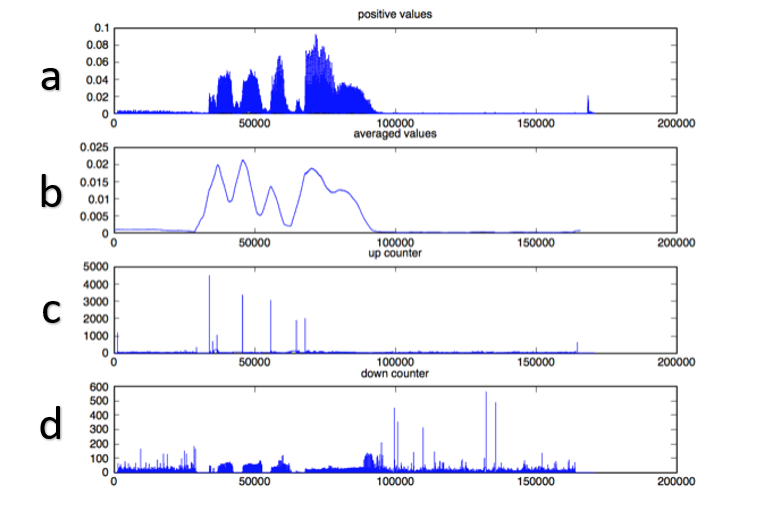
\includegraphics[width=9cm]{thesis/images/corr00}\\
  \caption{(a) Positive values of original waveform (b) Filtered values (c) Peak counter (d) Trough counter}\label{fig_c3_exp02}
\end{figure}
\subsubsection{Auto-correlation}
At the auto-correlation stage estimated phoneme segment boundaries are stored in an array and cross-correlated with the original signal.  Even though at a top-level view, the entire signal is auto-correlated, at the individual segment level, the signals are cross correlated against one another.  Furthermore, to achieve a ‘fair’ correlation estimate, individual segments representing estimated phonemes need to be re-sampled to eliminate mismatching of contour representations of the individual phonemes.\textcolor{blue}{  This was achieved by the filtering done at the segmentation stage.  Figure \ref{fig_c3_exp03} below shows sample auto-correlation result for the first peak-to-trough segment.}
\begin{figure}
\centering
  % Requires \usepackage{graphicx}
  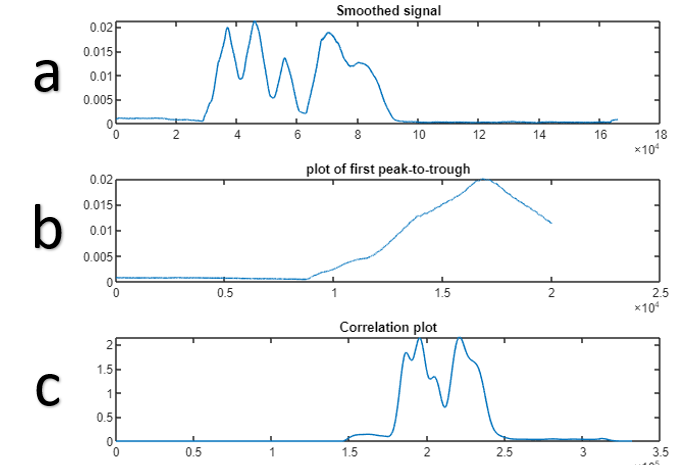
\includegraphics[width=9cm]{thesis/images/corr01}\\
  \caption{(a) Positive values of original waveform (b) Isolated Segment plot (c) Correlation plot of (a) against (b) plot. counter}\label{fig_c3_exp03}
\end{figure}

\startblue
Figure \ref{fig_c3_exp03}(a) is the smoothed signal from the segmentation procedure.  Figure \ref{fig_c3_exp03}(b) is the first peak to trough indicating the first phoneme in the utterance, and Figure \ref{fig_c3_exp03}(c) shows the auto correlation plot.  From Figure \ref{fig_c3_exp03}(c), it can be seen from the twin peaks in the cross-correlation plot indicates that the phoneme-pair in the first peak-to-trough segment was discovered twice within the signal.  This can form the basis of the phoneme's posterior distribution. Determining if there was a way of improving the accuracy of phoneme detection was not within the scope of this research.

The proposed auto-correlation algorithm performs both top-down and bottom-top processing.  In the first stage it does bottom-top segmentation, while in the second phase top-bottom auto-correlation.   The major weakness of this auto-correlation method is the lack of context between the phonemes.  For example consonants, which comprise non periodic noise signals, will be difficult to detect without the context of surrounding preceding and succeeding phonemes to the extent of a phrase-level of proximity context phonemes.  These contextual relationships can not be resolved in shallow systems such as this.  The Bayesian method of segmentation \citep{kamper2016unsupervised}, provides an alternative method which seeks to improve on these weaknesses using ASR feature preprocessing.  In this scheme, a combination of acoustic embedding and Dynamic Time Warping (DTW) for clustering is employed to replace auto-correlation.  In essence, it is beneficial to perform clustering on extracted features with less intrinsic noise than using an only smoothed audio data.\stopblue

\subsection{Experiments with Nao robot}
Nao is a humanoid robot developed mainly for deployment in environments for robotics education and development purposes.  Nao comes with a speech recognition software that offers features such as language settings and recognition sensitivity.  However it was understandably found to be limited because the Nao robot itself does not possess the processing power to perform CPU intensive training of acoustic models.  The Nao robot did however offer a level of support for using the pocketsphinx system. The pocketsphinx system is the C-language equivalent of CMUSphinx speech recognizer system also by Carnegie Mellon University.  Using the pocketsphinx method, acoustic models trained high performance systems can then be deployed to Nao for fast decoding within the Nao.  

\subsection{Digit Speech Recognition and Alignment Experiments}\label{sec_digitspeech}
These experiments were performed using CMU Sphinx4 recognition system and Kaldi speech recognition software.  While CMU Sphinx and pocketsphinx delivered standard interface for speech recognition using generative hybrid models, Kaldi speech in addition also offered advanced methods such as subspace Gaussian mixture model used to develop cross-lingual acoustic models and deep architectures for hybrid generative-discriminative models for speech recognition.   The main challenge with Kaldi was that it was CPU intensive and required a reasonable amount of parallel processing to achieve good results within a reasonable time period. 

Speech alignment experiments were performed using the Alisa \cite{stan2016alisa} tool which is a python based tool with calls made to the HMM toolkit \cite{young2002htk}.  The Alisa tool alignment process undergoes a semi-supervised process and requires an error prone time-intensive manual pre-alignment procedure.  The tool itself was found to be quite unstable and the output results were not very easily reproducible for further tests to be carried out on different data sets.  In addition, the time-intensive pre-alignment procedure made the tool not very useful for this research. Had the tool been more successful, the tool, which utilises \acrfull{vad} algorithms, would have been especially useful for sentence segmentation of long sequences of transcribed audio speech.  This tool however still lacked in alignment at either a word-level or sub-word level of alignment required in ASR pipelines.

\startblue
\section{Sequence-to-sequence Model Experiments}\label{sec_postalign}
A significant issue arises when using HMM-based toolkits such as Kaldi in low resource \acrshort{asr} applications.  This is the requirement for aligned speech.  In more recent endeavours, there have been efforts towards automatic alignment of transcribed audio speech recordings through successive Baum-Welch estimation techniques \citep{gales2014speech,ragni2018automatic,ragni2014data}. However, this technique is not particularly compatible with end-to-end goals adopted for this research as it would require preprocessing and successive pre-training of the data set.


The following section introduces \acrshort{rnn} sequence-to-sequence modelling and some of the pilot studies done using these models and in Chapters \ref{ch6_speech} and \ref{ch8_future}, how these methods deal with the problem of automatic speech alignment in a fashion which is compatible with end-to-end speech processing.  The end-to-end requirements were desirable for low-resource speech recognition as it introduces a simpler speech model design.  The downside however to the end-to-end approach is the dependency on very deep recurrent neural network structures which require large volumes of data for successful training.


In the wild, three types of naturally occurring sequence relationships exist: the one-to-many relationship also referred to here as \acrfull{simo}; the many-to-one relationship also referred to here as \acrfull{miso}, and; the many-to-many also referred to here as \acrfull{mimo}.  The one-to-one relationship also referred to as \acrfull{siso} is excluded here.  Although the \acrshort{siso} relationship is a naturally existing relationship, this relationship is not a sequence-type relationship and will not be modelled using a \acrlong{rnn}, but rather, can be modelled using regular \acrlong{dnn}s.  In addition, the \acrshort{mimo} relationship can be further subdivided into synchronous and asynchronous \acrshort{mimo}. In synchronous \acrshort{mimo}, the inputs and the outputs have equal lengths but in the asynchronous \acrshort{mimo}, the input and the output lengths are not necessarily equal.

\begin{figure}
\centering
  % Requires \usepackage{graphicx}
  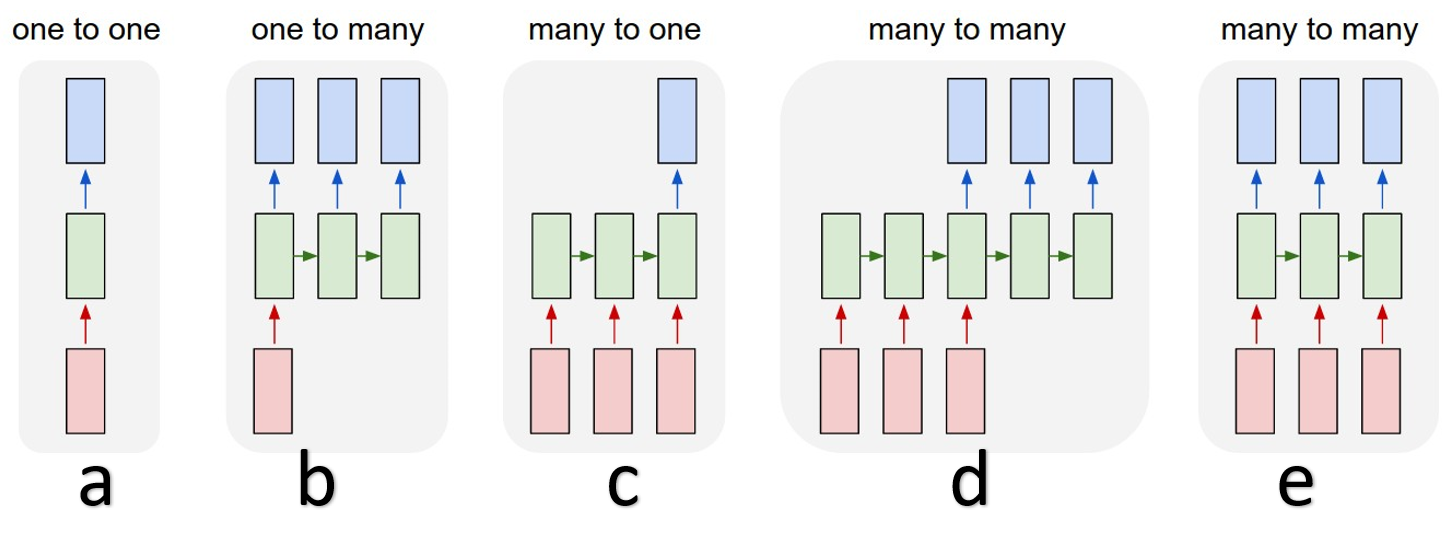
\includegraphics[width=14cm]{thesis/images/seq03.PNG}\\
  \caption{Relationship Types and their neural network interpretation.  \citep{karpathy2015unreasonable}}\label{fig_c3_seq2seq}
\end{figure}

Figure \ref{fig_c3_seq2seq} illustrates how the five  relationship types are translated into neural networks where (\ref{fig_c3_seq2seq}a) refers to a regular \acrshort{dnn} structure and (\ref{fig_c3_seq2seq}b to d) are different \acrshort{rnn} structures. Examples of each type of relationship structure are given in \cite{karpathy2015unreasonable}.  In Figure \ref{fig_c3_seq2seq}, the red blocks at the bottom are input blocks, the green blocks are neural network units and the blue blocks are output blocks.  For \acrshort{simo} relationship (Figure \ref{fig_c3_seq2seq}b), A single input will generate a sequence as output. An example of a \acrshort{simo} is an image captioning task where a single image input will generate a sentence or sequence of words. For the case of the \acrshort{miso} (Figure \ref{fig_c3_seq2seq}c), a sequence of inputs will generate a single output.  As an example, consider a fault detection task where a sequence of historical data can classify whether an instrument is faulty or not.  In this research, we only implement asynchronous \acrshort{mimo} (Figure \ref{fig_c3_seq2seq}d) and synchronous \acrshort{mimo} (Figure \ref{fig_c3_seq2seq}e) which satisfied the design requirement of the models implemented. In the asynchronous case (\ref{fig_c3_seq2seq}d), we see here that due to the misaligned or jagged alignment of inputs to outputs, there is a degree of freedom between the inputs and outputs such that they do not have to have equal number of inputs and outputs.  Within the \acrshort{rnn} model, this is implemented using two different \acrlong{rnn}s. One \acrshort{rnn} for the inputs known as the encoder network and one \acrshort{rnn} for the output known as the decoder network.  Together these encoder and decoder networks become a \acrshort{rnn}-Transducer network.   For the synchronous \acrshort{mimo} in Figure (\ref{fig_c3_seq2seq}e), however, only one \acrshort{rnn} is implemented constraining the number of inputs to be equal the number of outputs.  Note that both \acrshort{miso} and \acrshort{simo} are also implemented with a single \acrshort{rnn} structure, the difference between \acrshort{miso}, \acrshort{simo} and synchronous \acrshort{mimo} is that for \acrshort{simo} and \acrshort{miso} the corresponding inputs or outputs are ignored.  For the \acrshort{simo}, we only input the first \acrshort{rnn} sequence and ignore the rest.  For the \acrshort{miso} sequence, we only harvest the last output and ignore the preceding sequence of outputs.  

\subsection{Procedure for designing sequence-to-sequence \acrshort{rnn} models}\label{sec_341_rnnproc}
In the next two sections (\ref{sec_c2d} and \ref{sec_c3_g2p}), two pilot study experiment designs are discussed.  These experiments had two objectives; the first objective was to implement regular speech-recognition tasks using sequence-to-sequence methods and second objective was the exploration of sequence network designs described in the previous Section (\ref{sec_postalign}).  Since these experiments were mere pilot studies and not required in the final outputs, the results were not improved upon and were reserved for further investigation in future publications and the emphasis of these experiments was centred on sequence modelling design and implementation.  A detailed discussion of the final sequence models designed in this thesis is reserved for Chapters \ref{ch6_wlm} and \ref{ch6_speech}.  Generally for the sequence-to-sequence model experiments designed in this thesis we follow the following steps.
\begin{itemize}
    \item Step 1: Select the sequence \acrshort{rnn} model that satisfies the requirement for the sequence relationship being modelled.
    \item Step 2: Select an appropriate \acrshort{rnn} (see Chapter \ref{ch3RNN} for discussion of \acrshort{rnn} types) for each \acrshort{rnn} component.
    \item Step 3: Design neural network components including
    \begin{enumerate}
        \item Number of hidden layers
        \item Number of neurons in hidden layers
        \item Network saturation parameters
        \begin{itemize}
            \item Weight initialisation
            \item Non-linear function
            \item Number of epochs
            \item Learning rate
            \item Cost function
            \item Optimiser
        \end{itemize}
    \end{enumerate}
    \item Step 4: Design Regularisation measures.  These are measures to ensure your network, which can be viewed as a high dimension function fitter does, not over-generalise or under-generalise.
\end{itemize}

Note that in this research, parameters in steps 3 and 4 are either experimentally determined or selected based on similar research which has yielded the desired outcomes.

\stopblue

\subsection{Sequence-to-sequence character-to-diacritically-labelled-character model}\label{sec_c2d}
Experiments performed in this and the next three sections are all based on sequence-to-sequence modelling using recurrent neural networks.  \textcolor{blue}{While this section and the next section represent precursor experiments centred around sequence modelling for speech recognition tasks, sections \ref{sec_grulm} and \ref{sec_be2e} introduce the major experiments in this work later discussed in Chapters \ref{ch6_wlm} and \ref{ch6_speech}.}

\startblue
The character-to-diacritically labelled character model was a sequence-to-sequence diacritically labeled experiment to automatically infer diacritic transcriptions of the Wakirike language given the plain unmarked Wakirike language text as input.  This is a task, when achieved successfully, then becomes a sub task towards developing a phonetic dictionary for the Wakirike Language and the phonetic dictionary in turn can be used in HMM speech recognition or as post-processing technique for an end-to-end model output text.  This experiment follows the design procedure outlined in Section \ref{sec_341_rnnproc}. Figure \ref{fig_c3_t2d_sample} gives example input and output sequences for this experiment.

\begin{figure}
\centering
  % Requires \usepackage{graphicx}
  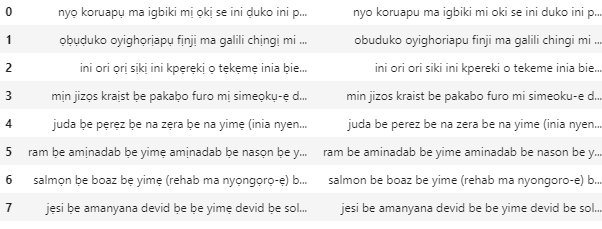
\includegraphics[width=14cm]{thesis/images/diacritic.png}\\
  \caption{Diacritic symbol generator training data sequences}\label{fig_c3_t2d_sample}
\end{figure}

Although after training for 75 epochs (Figure \ref{fig_c3_t2d00}) the accuracy of the Wakirike diacritics sequence generator model was still unacceptable (6\%), the model may have been improved by changing the sequence-relationship model from an asynchronous \acrshort{mimo} to a synchronous \acrshort{mimo} sequence model.  Improvements from a synchronous design stems from the insertion and deletion errors observed from the output transcription.  Ensuring the outputs and inputs had equal length would therefore constrain the model for better results.  The main aim of the pilot experiment, however, was to implement asynchronous transducer \acrshort{rnn} design and therefore further experiments for the diacritics sequence generator were not done.
\stopblue
\begin{figure}
\centering
  % Requires \usepackage{graphicx}
  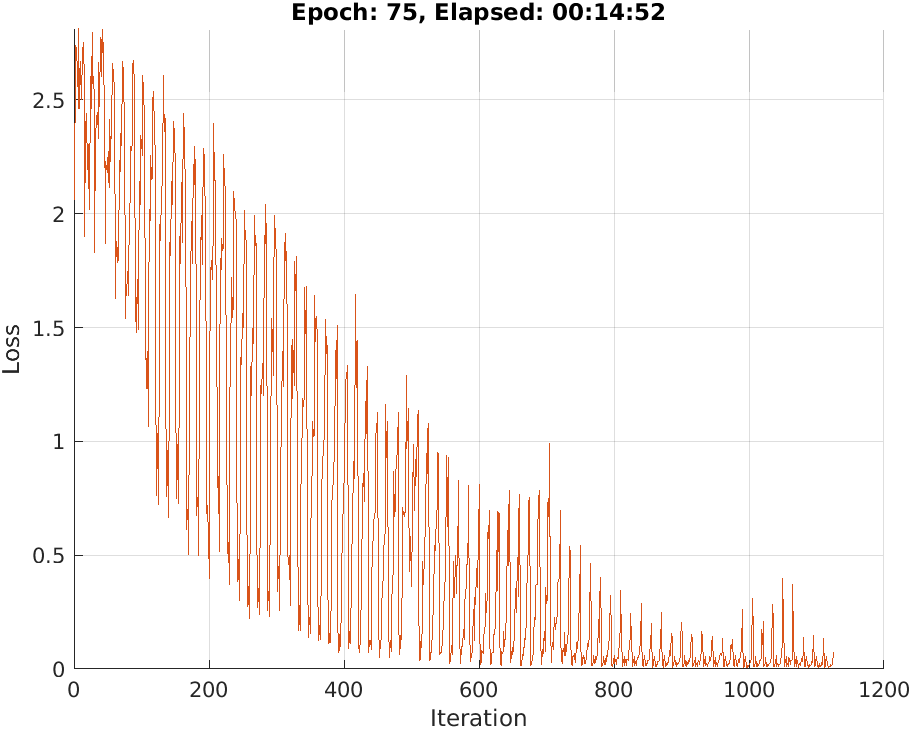
\includegraphics[width=14cm]{thesis/images/dtrain.png}\\
  \caption{Diacritic symbol generator model training loss}\label{fig_c3_t2d00}
\end{figure}

\subsection{Sequence-to-sequence Grapheme-to-Phoneme (G2P) model}\label{sec_c3_g2p}
This follow up experiment to the previous experiment in section \ref{sec_c2d},  attempts to automatically generate a phonetic dictionary from graphemes in a text corpus. Grapheme-to-phoneme experiments come in two flavours, the first being a continuation of the previous experiment, that is, using diacritically marked symbols, and the second flavour using non-marked graphemes as input.  The experiments performed used the latter non-marked graphemes as input.  \textcolor{blue}{For this experiment, a pre-trained model having a 2-layer transducer \acrshort{rnn} having 256 hidden units was fine-tuned on the training data.  Appendix V shows the output Wakirike phonetic dictionary generated from this experiment.}

What follows in the next three sections are sequence-to-sequence experiments actively developed in this research and are detailed in chapters (\ref{ch6_wlm} and \ref{ch6_speech}).  A brief summary of the experiments are highlighted in the following sections (\ref{sec_grulm}, \ref{sec_be2e} and \ref{c3sec_espnet}).  Note that these models all utilise TensorFlow deep learning library including the Bi-directional speech model (section \ref{sec_be2e}) which is built on top of Mozilla DeepSpeech with the exception of section \ref{c3sec_espnet} which is based on PyTorch; a  python library having deep learning features identical  to that of TensorFlow.

\subsection{GRU language model for Wakirike language based on TensorFlow}\label{sec_grulm}
The language model developed in this research is a character-based sequence-to-sequence deep recurrent neural network that maps a sequence of characters to a sequence of words found in the training data set. This model met the objective of reducing the vocabulary size required for language models as well as the text corpus required as inferences could be made over the smaller-fixed character vocabulary rather than orders or magnitude larger word corpus with the possibility of out of vocabulary terms found in the training data.  Though this may occur in the character sequence-model at the inference stage, it would not normally happen during training.  The neural network model developed is described in Chapters \ref{ch3RNN} and \ref{ch6_speech}, and consists of Gated Recurrent Unit (GRU) Recurrent Neural Network (RNN). The GRU is a specialised type of Long Short-Term Memory (LSTM) cell RNN.  The emphasis here is on the ability to model over particularly long sequences of the training data.  In this case, over long character sequences.  Thus, the network is able to learn long term dependencies as would be naturally required to construct grammatically correct sentences.  In essence, the RNN is able to learn grammar rules inherently from the training data.

\subsection{Bi-Directional LSTM-based end-to-end speech model}\label{sec_be2e}
A similar LSTM sequence-to-sequence network based on Baidu Research’s original research design \citep{hannun2014deep} is developed in this research for end-to-end speech recognition.  This model, as its name implies, attempts to establish long term relationships by adding a reinforcing LSTM layer learning information but this time from the opposite direction, hence the bi-directional architecture.  

In addition, the model incorporates the Connectionist Temporal Classifier (CTC) decoder. This enables the model to make run-time inferences on both the character as well as estimate audio wave to character label alignment simultaneously.  This makes this design accommodate end-to-end goals and ultimately simplifies the overall design and completely eliminates the need for either manual or semi-supervised alignments mentioned previously in sections (\ref{sec_c3_alisa}, \ref{sec_digitspeech} and \ref{sec_postalign}).

\subsection{ESP-Net Experiments}\label{c3sec_espnet}
The ESP-Net (End-to-end Speech Network) toolkit \citep{watanabe2018espnet}, is a speech processing toolkit that was of interest to this research because it offers end-to-end capabilities not only in \acrfull{asr} but also in \acrfull{tts} or speech synthesis and other speech-sequence-processing related tasks.  In addition, the toolkit offers multi-modal training combining both Attention networks \citep{vaswani2017attention} with CTC Transformer networks as well as multi-channel feature representation that is, the fusing together of multiple feature representations of an audio signal.

\section{Method of evaluation}
System building methodology \citep{nunamaker1990systems} for speech recognition systems requires models to be evaluated against speech recognition Machine Learning metrics.  For language models, perplexity metric was used for evaluation.  \acrfull{bleu}\citep{papineni2002bleu} has also been used as a metric for evaluating language models.

Perplexity measures the complexity of a language that the language model is designed to represent \citep{1976jelinekcontinuous}. In practice, the entropy of a language with an N-gram language model $P_N(W)$ is measured from a set of sentences and is defined as
\begin{equation}H=\sum_{\mathbf{W}\in\Omega}P_N(\mathbf{W})
\label{eqn_c2_lm05}
\end{equation}

where $\Omega$ is a set of sentences of the language. The perplexity, which is interpreted as the average word-branching factor, is defined as
\begin{equation}PP(W)=2^H
\label{eqn_c2_lm06}
\end{equation}
where H is the average entropy of the system or the average log probability defined as
\begin{equation}
H=-\frac{1}{N}\sum_{i=1}^N[log_2P(w_1,w_2\dots w_N)]
\label{eqn_c2_lm07}
\end{equation}
For a bi gram model therefore, equation (\ref{eqn_c2_lm07}) becomes
\begin{equation}
PP(W)=2^H=2^{-\frac{1}{N}\sum_{i=1}^N[log_2P(w_1,w_2\dots w_N)]}
\label{eqn_c2_lm08}
\end{equation}
After simplifying we have
\begin{equation}
PP(W)=\sqrt[N]{\prod_{i=1}^N\frac{1}{P(w_i|w_{i-1})}}
\label{eqn_c2_lm09}
\end{equation}


Full speech recognition pipelines are usually evaluated against the Word Error Rate (WER).  WER is computed as follows:
\begin{equation}\label{eqn_2_3_wer}
WER=\frac{I+D+R}{WC}\times 100
\end{equation}
Here $I,D,$ and $R$ are wrong insertions, deletions and replacements respectively and $WC$ is the word count.

Metrics used for low speech recognition in the zero speech challenge \citep{versteegh2015zero} include the ABX metric. Other common speech recognition error metrics following a similar definition as the Word Error Rate (WER) are Character Error Rate (CER), Phoneme Error Rate (PER) and Syllabic Error Rate (SyER) and sentence error rate (SER).

\section{Chapter Summary}
In this chapter we outline how this research set out to achieve its objectives.  The main claim of this research is that by building a speech model that combines knowledge of end-to-end processing along with state of the art signal processing, the overall training complexity and build time for new ASR systems can be improved.  This research aims to deliver this through by the unique combination of a CTC-based deep recurrent bi-directional neural network with high performance feature processing of Deep Scattering Networks (DSNs).

This chapter also reviews the technologies utilised by this research in order to arrive at the research outputs and briefly describes the experiments performed.  Within this space we describe CMUSphinx, Kaldi, Mozilla DeepSpeech, TensorFlow, Matlab and ScatNet as major libraries used.   The first two of these are Hidden Markov Model (HMM)-based libraries and the rest are  signal processing systems used to build Deep Recurrent Neural Network (RNN) models. Finally,  metrics for the evaluation of the models built in this research is discussed.


\chapter{Recurrent Neural Networks in Speech Recognition}\label{ch3RNN}
The HMM model described in Chapter \ref{c02} uses a divide and conquer strategy which has also been described as a generative Machine Learning algorithm in which we use the smaller components’ representations as modelled by the HMM to learn the entire speech process.   In previous chapters, this was referred to as the bottom-top strategy.  The discriminative method however uses the opposite mechanism.  Instead of using the building blocks of speech to determine speech parameters of a HMM, the discriminative strategy determines the posterior probability directly using the joint probability distribution of the parameters involved in the discriminative process.  The discriminative approach, discussed in this chapter focuses on Neural network architectures.

\section{Neural network architecture}

The building block of a neural network simulates a combination of two consecutive linear and non-linear operations having many inputs interconnected with the linear portion of the network.  This rudimentary structure is described by McCullough and Pitts (1942) and in  \cite{cowan1990discussion} as the Perceptron in Figure \ref{fig_3_1_ptron} 

\begin{figure}
\centering
  % Requires \usepackage{graphicx}
  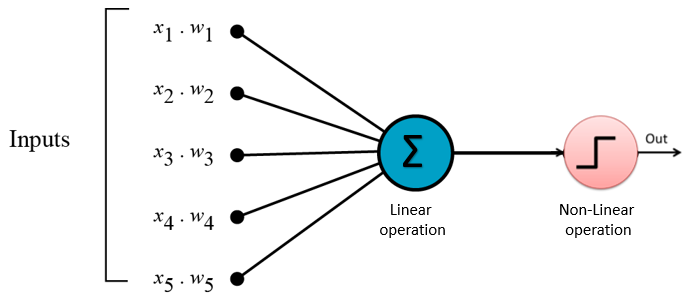
\includegraphics[width=7cm]{thesis/images/ptron2.png}\\
  \caption{Perceptron algorithm where $x_i$ are inputs and $w_i$ are input weights} \label{fig_3_1_ptron}
\end{figure}

The linear operation is the sum of the products of the input feature and a  weight vector set.  This vector sum of products is referred to as an affine transformation or operation.  The non linear operation is given by any one of a selection of nonlinear functions.  In  Figure \ref{fig_3_2_nn} this is shown as a step function.  The step function is activated (becomes 1) whenever the output of the linear function is above a certain threshold, otherwise remains at 0.  A simple neural network of perceptrons is formed by stacking the perceptrons into an interconnected layer as shown in the Figure \ref{fig_3_2_nn}.

\begin{figure}
\centering
  % Requires \usepackage{graphicx}
  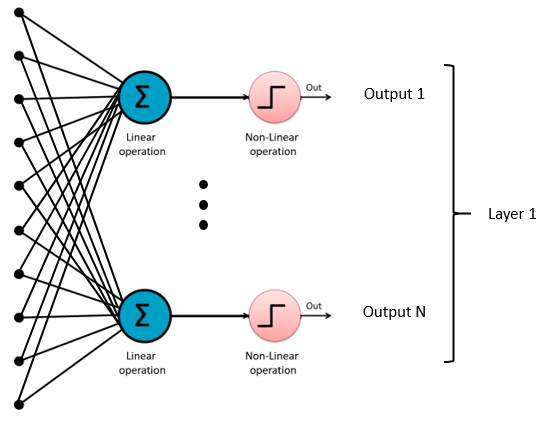
\includegraphics[width=7cm]{thesis/images/ptron3.png}\\
  \caption{Neural network} \label{fig_3_2_nn}
\end{figure}

From the preceding paragraph, each combination of linear operation followed by a non linear operation is called a neuron and the total number of neurons in the layer formed is termed as $M$-number of neurons in the layer.

\subsection{Multi-layer Perceptron (MLP)}
The multilayer Perceptron or MLP extends the basic Perceptron structure by adding one or more hidden layers.  These hidden layers comprise the outputs of one layer becoming the input of the next layer. In the simplest case having one hidden layer, the output of layer 1 becomes the input of the final output layer.  In comparison, the Perceptron is a one dimensional structure having one or more linear and non linear combination outputs, while the multilayer Perceptron is a 2-dimensional structure having one or more hidden layers of $N$ linear and non-linear combination outputs.  Mathematically speaking the output of each layer of an MLP having $N$ inputs and $M$.  The nonlinear portion of this equation is given by
\begin{equation}
z_j=h(b_j)=\frac{1}{ 1+e^{-b_j}} 
\label{eqn_c3_nn_01}
\end{equation}
 The other linear half of the equation is given by:
\begin{equation}
b_j=\sum_{i=0}^Nw_{ji}^{(1)}\qquad j=1,2,\dots,M
\label{eqn_c3_nn_02}
\end{equation}

For each layer in the MLP, the zeroth input value $x_0$ is 1 indicating a bias term.  This bias term is used in the neural network to ensure regularised and expected behaviour of the neural network.  In this example the non-linear step function is given by a more complex exponential.  In the next section the nonlinear functions for a multilayer Perceptron is derived.
\subsection{Sigmoid and soft-max Activation Function}
The combination of the linear function and the non linear function in the neural network could be said to be transformation of an algebraic problem to a probabilistic function.  In this case the "step" function is a squashing sigmoid-shaped function that converts the inputs into a Naive Bayes function evaluating the probability that an output belongs to any of the output classes $(C_y)$ given the data $(\mathbf{x})$.
\begin{equation}
p(C_1|\mathbf{x})=f(a)=f(\mathbf{w^\top x}+w_0)
\label{eqn_c3_nn_02}\end{equation}
In a two class problem with classes $C_1$ and $C_2$, the posterior probability of class $C_1$ is expressed using Bayes’s theorem
\begin{equation}
p(C_1|\mathbf{x})=\frac{p(\mathbf{x}|C_1)p(C_1)}{p(x|C_1)p(C_1)+p(\mathbf{x}|C_2)p(C_2)}
\label{eqn_c3_nn_03}\end{equation}
Dividing through by $p(\mathbf{x}|C_1)p(C_1)$ gives us
\begin{equation}
p(C_1|\mathbf(x)=\frac{1}{1+\frac{p(\mathbf{x}|C_1)p(C_1)}{p(\mathbf{x}|C_2)p(C_2)}}
\label{eqn_c3_nn_04}\end{equation}

If we define the ratio of the log posterior probabilities as
\begin{equation}
a=\ln\frac{p(\mathbf{x}|C_1)p(C_1)}{p(\mathbf{x}|C_2)p(C_2)}
\label{eqn_c3_nn_05}\end{equation}
If we substitute back into (4) we have:

\begin{equation}p(C_1|\mathbf{x})=f(a)=\frac{1}{1+e^{-a}}
\label{eqn_c3_nn_06}
\end{equation}

Here $a=\mathbf{w^\top x}=w_0$.  Thus the activation for the non-linear function is driven by the probability of the data to give the output class.  The probabilistic function here is called a sigmoid function due to the s-shaped graph that is plotted by the function.

Rather than using the sigmoid function for multi-class classification a similar soft max function is derived by using the log probability of classes. If $a_k=\ln(p(\mathbf{x}|C_k)p(C_k))$ then:
\begin{equation}
y_k=p(C_k|\mathbf{x})=\frac{e^{a_k}}{\Sigma_{\ell=1}^K e^{a_\ell}}
\label{eqn_c3_nn_07}\end{equation}
\begin{equation}
a_k=\sum_{i=0}^dw_{ki}x_i
\label{eqn_c3_nn_08}\end{equation}

Recall that in the generative classification method the problem is divided into sub problems by using the conditional probability, while in the discriminative approach the joint probability is determined by looking at the data directly.  This is what $p(C_k|\mathbf{x})$ represents.  However also, recall that we still need to determine the correct probability distribution represented by the data.  This is achieved by determining the values of the weights of the linear operation.  In the next section a method known as back propagation is discussed.  Back propagation is the training algorithm used to determine the weight vector of all the layers in the neural network.  Back propagation is an extension of the Gradient descent algorithm.

\subsection{Back propagation algorithm (backprop)}
In the previous section, the neural network architecture has been described as having $N$ inputs $M$ neurons and $L$ layers. Each layer comprises $M$ neurons of a maximum of $N$ inputs times $M$ neurons interconnections which embodies the inner product of the inputs and unknown set of weights. The output of this inner product is then passed to a logistic squashing function that results in the output probabilities.  The discriminative process is used here to determine the correct combination of weight vectors that accurately describe the training data.  For neural networks, the weight vectors at each layer are determined through propagating the errors back through each preceding layer and adjusting the weights according to the errors propagated each time a batch of the data is processed.  This process of continuously adjusting weights from back propagation continues until all the data is processed and a steady state has been reached.  The steady state refers to the fact that the error has reached a steady and/or acceptable negligible value.  This is often referred to in Machine Learning as convergence \citep{boden2002guide}.

\subsection{Gradient Descent}
The last section ended stating that the back-propagation algorithm is an extension of the gradient descent algorithm.  It has also been seen that back propagation works by propagating the error and making adjustments on the weights.  In this section, the Gradient Descent algorithm is reviewed and how it is used in back propagation is examined.  

The concept behind the Gradient descent algorithm is the fact that a function is optimized when the gradient of the function is equal to $0$.  Gradient descent algorithm is significant in Machine Learning applications because a cost function is easily defined for a particular Machine Learning application that is able to determine the error between the predicted value and the actual value.  Then, the parameters of the problem can be adjusted until the derivative of the cost function using gradient descent is zero.  Thus the Machine Learning algorithm adjusts its parameters until the error is minimised or removed.

A common error function or cost function for neural networks is the sum-of-squares error cost function.  This is obtained by summing the difference between the actual value and the Machine Learning model value over the training set $N$. 
\begin{equation}
E^n=\frac{1}{2}\sum_{k=1}^K(l_k^n-y_k^n)^2
\label{eqn_c3_nn_09}\end{equation}
where $l$ is the label value for the output value $y$.

In a neural network having a weight matrix $\mathbf{W}$ of $M$ neurons times $N$ inputs, the resulting gradient is a vector of partial derivatives of $E$ with respect to each element.  
\begin{equation}\nabla_{\mathbf{W}}E=\left(\frac{\partial E}{\partial w_{10}},\dots,\frac{\partial E}{\partial w_{ki}},\dots,\frac{\partial E}{\partial w_{Kd}}\right) 
\label{eqn_c3_nn_10}\end{equation}

The adjustment on each weight therefore on each iteration is:
\begin{equation}
w_{kj}^{\tau+1}=w_{kj}^{\tau}-\eta\frac{\partial E}{\partial w_{kj}}
\label{eqn_c3_nn_11}\end{equation}

Where $\tau$ is the iteration and $\eta$ is a constant learning rate which is a factor to speed up or slow down the rate of learning of the Machine Learning algorithm which in this case is the neural network.

\section{RNN, LSTM and GRU Networks}
Neural networks have become increasingly popular due to their ability to model non-linear system dynamics. Since their inception, there have been many modifications made to the original design of having linear affine transformations terminated with a nonlinear functions as the means to capture both linear and non-linear features of the target system. In particular, one of such neural network  modifications, namely the recurrent neural network, has been shown to overcome the limitation of varying lengths in the inputs and outputs of the classic feed-forward neural network.  In addition the RNN is not only able to learn non-linear features of a system but has also been shown to be effective at capturing the patterns in sequential data.  This section develops recurrent neural networks (RNNs) from a specialised multi-layer Perceptron (MLP) or the deep neural network (DNN).

\subsection{Deep Neural Networks (DNNs)}\label{dnn}

Deep neural networks have been accepted to be networks having multiple layers and capable of hierarchical knowledge representation \citep{yu2016automatic}.
 This will therefore include multi-layer Perceptrons (MLPs) having more than one hidden layer \citep{dahl2012context} as well as deep belief networks (DBNs)\citep{mohamed2009deep,yu2010roles} having a similar structure.  Therefore, following the MLP architecture, A DNN uses multiple hidden layers and generates distribution function, $p(c|x_t)$ on the output layer when an input vector $\mathbf{x}_t$ is applied.  At the first hidden layer, activations are vectors evaluated using
\begin{equation}\mathbf{h}^{(1)}=\sigma(\mathbf{W}^{(1)T}\mathbf{x}_t+\mathbf{b}^{(1)})
\label{eqn_c3_dnn01}\end{equation}
The matrix $\mathbf{W}^{(1)}$ is the weight matrix and vector $b^{(1)}$, the bias vector for the layer.  The function $\sigma(\cdot)$ is the point-wise non-linear function.
DNNs activations $h^{(i)}$ at layer i, at arbitrarily many hidden layers after the first hidden layer, are subsequently hidden activations are determined from
\begin{equation}\mathbf{h}^{(1)}=\sigma(\mathbf{W}^{(1)T}\mathbf{h}^{(i-1)}+\mathbf{b}^{(1)})
\label{eqn_c3_dnn02}\end{equation}
The distribution over all the possible set of characters $c$ is obtained in the final layer of the network in the exact way of a multi-layer Perceptron, that is, using soft max activation at the output layer of the form,
\begin{equation}p(c=c_k|x_t)=\frac{exp(-(\mathbf{W}^{(s)T}_kh^{(i-1)}+b_k^{(1)}))}{\sum_j exp(-(\mathbf{W}^{(s)T}_kh^{(i-1)}+b_k^{(1)}))}
\label{eqn_c3_dnn03}\end{equation}
$W_k^{(s)}$ and $b_k^{(k)}$ respectively are the output weight matrix and the scalar bias term of the $k$-th neuron. Accordingly, sub gradients for all parameters in the DNN are utilised to back propagate errors in weights during training for gradient-based optimisation techniques.  In DNN-HMM speech models,   DNNs are trained to predict probability distributions over senones.  However, in the model neural network described in section \ref{c3_ctc}, of this thesis, predicts per character conditional distributions.
Combining equations (\ref{eqn_c3_nn_11}, \ref{eqn_c3_dnn01}, \ref{eqn_c3_dnn02} and \ref{eqn_c3_dnn03}) the following simplified algorithm ensues

\begin{algorithm}[H]
\SetAlgoLined
\KwResult{Optimal weights }
 initialise weights randomly\;
 \While{error is significant or epochs less than maximum}{
  forward computation in equation (\ref{eqn_c3_dnn01} and \ref{eqn_c3_dnn02} )\;
  determine layer wise error for weights and biases $\Delta_\mathbf{W}E$ and  $\Delta_\mathbf{b}E$ \;
  update weights and biases according to gradient descent. Equation (\ref{eqn_c3_nn_11});
 }
 \caption{DNN training algorithm}
\end{algorithm}

\subsection{Recurrent Neural Networks}
One of the two advantages RNNs have over regular DNNs is the ability to capture varying lengths of outputs to inputs.  That is for tasks such as language translation where there is no one to one correspondence of number of words in a sentence for example from the source language to the output destination language.  At the same time the sentence length appearing at the input and that appearing at the output differ for different sentences.  This is the first problem of varying lengths for input and output sequences.

The second issue that RNNs effectively contain as opposed to DNNs is capturing temporal relationships between the input sequences.  As was realised for hidden Markov models, it was seen that the HMM modeled not just observation likelihoods but also transition state likelihoods which were latent or hidden variables.  By tying the output of previous neuron activations to present neuron activations, a DNN inherits a cyclic architecture becoming a recurrent neural network (RNN). As a result, an RNN is to able capture previous hidden states and in the process derive memory-like capabilities \citep{yu2016automatic}.

In speech processing, it is observed that for a given utterance, there are various temporal dependencies which may not be sufficiently captured by DNN-based systems because DNN systems ignore previous hidden representations and output distributions at each time step $t$.  The DNN derives its output using only the  feature inputs $x_t$. The architecture of RNN to enable better modelling of temporal dependencies present in a speech is given in \citep{hannun2014first, yu2016automatic}. 

\begin{equation}h_t^{(j)}=\sigma(\mathbf{W}^{(j)T}h_t^{(i-1)}+\mathbf{W}^{(j)T}_kh_{t-1}^{(j)}+b^{(j)}))
\label{eqn_c3_rnn01}\end{equation}

It can be seen in equation (\ref{eqn_c3_rnn01}) above that given a selected RNN  hidden layer $j$, a temporally recurrent weight matrix $W^{(f)}$ is computed for output activations $h^{(j)}_{t-1}$ for the hidden activation vector of layer $j$ at time step $t - 1$ such that the output contributes to the standard DNN output of  $\mathbf{W}^{(j)T}h_t^{(i-1)}$. It can also be seen from  equation (\ref{eqn_c3_rnn01}) that the temporal recurrent weight matrix computation is a modified version of the standard DNN weight matrix computation and that the overall output is a superposition of the two.

Since computations for a RNN are the same as those described in standard DNN evaluations, it is possible to compute the sub gradient for  RNN architecture using the back propagation algorithm.  The modified algorithm appropriately called back propagation through time (BPTT) \citep{boden2002guide,jaeger2002tutorial} is derived in section \ref{c3_BPTT} below.  

\subsection{Back propagation through time (BPTT) algorithm}\label{c3_BPTT}
First we define an arbitrary but carefully chosen number of time steps $t=1,2,\dots,T$ such that at each time step the states of the neuron activations $j=1,2,\dots,J$ are captured.
Using the sum-squared error as the cost function
\begin{equation}
E=c\sum_{t=1}^T||\mathbf{l}_t-\mathbf{y}_t||^2=c\sum_{t=1}^T\sum_{j=1}^L(l_t(j)-y_t(j))^2 \label{eqn_c3_bptt01}\end{equation}

Where $c$ is a gradient descent convenience factor in Equation (\ref{eqn_c3_bptt01}). $||\mathbf{l}_t-\mathbf{y}_t||$ is the modulus of the difference between the actual output $\mathbf{y}_t$ and the label vector $\mathbf{y}_t$ at time $t$. The two-step BPTT algorithm described in \cite{yu2016automatic} is involves the recursive computation of the cost function and updating of the network weights.

For each of these steps recall from equation (\ref{eqn_c3_rnn01}) the activation of a hidden layer is a result of the composition of the regular DNN activation and an activation generated from weights from the previous time step.

The error term at final time t=T is
\begin{equation}
\delta^y_T(j)=-\frac{\delta E}{\delta y_T(j)}\frac{\delta y_T(j)}{\delta v_T(j)}=(l_T(j)-y_T(j))g'(v_T(j))\text{ for } j=1,2,\dots,L \label{eqn_c3_bptt04}\end{equation}
or
\begin{equation}
\mathbf{\delta}_T^y=(\mathbf{l}_T-\mathbf{y}_T)\bullet g'(\mathbf{v}_T) \label{eqn_c3_bptt05}\end{equation}
The error at the hidden layer is given as
\begin{equation}
\delta_T^h(j)=-\left(\sum_{i=1}^L\frac{\partial E}{\partial v_T(i)}\frac{\partial v_T(i)}{\partial h_T(j)}\frac{\partial h_T(j)}{\partial u_t(j)}\right)=\sum_{i=1}^L\delta_T^y(i)w_{hy}(i,j)f'(u_T(j))\text{ for } j=1,2,...,N \label{eqn_c3_bptt06}
\end{equation}
or $\delta_T^h=\mathbf{W}_{hy}^T\mathbf{\delta}_T^y\bullet f'(\mathbf{u}_T)$
where $\bullet$ is element-wise multiplication.

The recursive component for other time frames, $t=T-1, T-2, …, 1,$ the error term is determined as

\begin{equation}
\delta_t^y(j)=(l_t(j)-y_t(j))g'(v_t(j))\text{ for } j=1,2,\dots,L
\label{eqn_c3_bptt07}\end{equation}
or \begin{equation}
\mathbf{\delta}_t^y = (\mathbf{l}_t-\mathbf{y}_t)\bullet g'(\mathbf{v}_t) \label{eqn_c3_bptt08}\end{equation}

Therefore the output units are

\begin{equation}\begin{aligned}\delta_t^h(j)&=-\left[\sum_{i=1}^N\frac{\partial E}{\partial\mathbf{u}_{t+1}(i)}\frac{\partial\mathbf{u}_{t+1}(i)}{\partial h_t(j)}+\sum_{i=1}^L\frac{\partial E}{\partial v_t(i)}\frac{\partial v_t(i)}{\partial h_t(j)}\right]\frac{\partial h_t(j)}{\partial u_t(j)}\\ &=\left[\sum_{i=1}^N\delta_{t+1}^h(i)w_{hh}(i,j)+\sum_{i=1}^L\delta_t^y(i)w_{hy}(i,j)\right]f'(u_t(j)) \text{ for }j=1,\dots,N \\ \text{ or } \delta_t^h&=\left[\mathbf{W}_{hh}^\top\mathbf{\delta}_{t+1}^h+\mathbf{W}_{hy}^\top\mathbf{\delta}_t^y\right]\bullet f'(\mathbf{u}_t)\end{aligned}\label{eqn_c3_bptt09}\end{equation}

Note that the error terms are propagated back from hidden layer at time frame $t + 1$ to the output at time frame $t$.

\subsubsection{Update of RNN Weights}
The weights are updated using the error terms determined in the previous section.  For the output weight matrices, we have 

\begin{equation}
\begin{aligned}w_{hy}^{new}(i,j)&=w_{hy}(i,j)-\gamma\sum_{t=1}^T\frac{\partial E}{\partial v_t(i)}\frac{\partial v_t(i)}{\partial w_{hy}(i,j)}=w_{hy}(i,j)-\gamma\sum_{i=1}^T\delta_t^y(i)h_t(j)\\ \text{ or }\mathbf{W}_{hy}^{new}&=\mathbf{W}_{hy}+\gamma\sum_{t=1}^T\mathbf{\delta}_y^t\mathbf{h}_t^\top\end{aligned} \label{eqn_c3_bptt10}\end{equation}

For the input weight matrices, we get \begin{equation}
w_{xh}^{new}(i,j)=w_{xh}(i,j)-\gamma\sum_{t=1}^T\frac{\partial E}{\partial u_t(i)}\frac{\partial u_t(i)}{\partial w_{xh}(i,j)}=w_{xh}(i,j)-\gamma\sum_{t=1}^T\delta_t^h(i)x_t(j) \label{eqn_c3_bptt11}\end{equation}

or 
\begin{equation}
\mathbf{W}_{xh}^{new}=\mathbf{W}_{xh}+\gamma\sum_{t=1}^T\mathbf{\delta}_h^t\mathbf{x}_t^\top \label{eqn_c3_bptt_13}\end{equation}

For the recurrent weight matrices we have 

\begin{equation} \begin{split}w_{hh}^{new}(i,j)&=w_{hh}(i,j)-\gamma\sum_{t=1}^T\frac{\partial E}{\partial u_t(i)}\frac{\partial u_t(i)}{\partial w_{hh}(i,j)}\\ &=w_{hh}(i,j)-\gamma\sum_{t=1}^T\mathbf{\delta}_h^t(i)h_{t-1}(j)\\ \text{ or }&=\mathbf{W}_{hh}^{new}=\mathbf{W}_{hh}+\gamma\sum_{t=1}^T\mathbf{\delta}_h^t\mathbf{h}_{t-1}^\top \end{split} \label{eqn_c3_bptt14}\end{equation}

In the BPTT algorithm the sub gradients are summed over all time frames. The algorithm is summarised below:

\begin{algorithm}[H]
\SetAlgoLined
\KwData{$\{\mathbf{x}_t,\mathbf{I}_t\} 1\le t\le T$ }
\KwResult{Optimal weights }
 //$\mathbf{x}_t$ is the input feature sequence
 //$\mathbf{I}_t$ is the label sequence\;
 initialise weights randomly\;
 \For{error is significant or epochs less than maximum}{
  \For{$t\leftarrow 1;t<=T;t\leftarrow t+1$ }{
    //forward computation \;
    $\mathbf{u}_t\leftarrow\mathbf{W}_{xh}+\mathbf{W}_{hh}\mathbf{h}_{t-1}$\; $\mathbf{h}_t\leftarrow f(\mathbf{u}_{t})
    $\; $\mathbf{v}_t\leftarrow \mathbf{W}_{hy}\mathbf{h}_{t}
    $\; $\mathbf{y}_t\leftarrow  g(\mathbf{v}_t)$
  }
  \Begin{//backprop through time \;
    $\mathbf{\delta}_T^y=(\mathbf{l}_T-\mathbf{y}_T)\bullet g'(\mathbf{v}_T)$\;
    $\delta_T^h&=\mathbf{W}_{hh}^\top\mathbf{\delta}_{t+1}^h+\mathbf{W}_{hy}^\top\mathbf{\delta}_T^y\bullet f'(\mathbf{u}_T)$\;
    \For{$t\gets T-t; t>=1; t\gets t-1$}{
      $\mathbf{\delta}_t^y=(\mathbf{l}_t-\mathbf{y}_t)\bullet g'(\mathbf{v}_t)$\;
      $\delta_t^h&=\left[\mathbf{W}_{hh}^\top\mathbf{\delta}_{t+1}^h+\mathbf{W}_{hy}^\top\mathbf{\delta}_t^y\right]\bullet f'(\mathbf{u}_t)$\;
    }
  }
  update weights and biases according to gradient descent\;
  \Begin{
    $\mathbf{W}_{hy}^{new}=\mathbf{W}_{hy}+\gamma\sum_{t=1}^T\mathbf{\delta}_y^t\mathbf{h}_t^\top$\;
    $\mathbf{W}_{hh}^{new}=\mathbf{W}_{hh}+\gamma\sum_{t=1}^T\mathbf{\delta}_h^t\mathbf{h}_{t-1}^\top$\;
  }
 }
 \caption{RNN training algorithm}
\end{algorithm}

\subsection{LSTMs and GRUs}

A special implementation of the RNN called the Long Short Term Memory (LSTM) has been designed to capture patterns over particularly long sequences of data and thus is an ideal candidate for generating character sequences while preserving syntactic language rules learned from the training data.

The internal structure and working  of the LSTM cell is documented by its creators in \cite{sak2014long}. The ability to recall information over extended sequences results from the internal gated structure which performs a series of element wise multiplications on the inputs and internal state of the LSTM cell at each time step.  In addition to the output neurons which in this text we refer to as the write gate and denote as the current cell state, $\mathbf{c}_t$, three additional gates (comprising a neural network sub-layer) located within the LSTM cell are the input gate, the forget gate and the output gate.  Together with the initial current state cell, these gates along with the current-state cell itself enable the LSTM cell architecture to store information, forward information, delete information and receive information.  Generally however, the LSTM cell looks like a regular feed-forward network having a set of neurons capped with a nonlinear function.  The recurrent nature of the network arises, however due to the fact that the internal state of the RNN cell is rerouted back as an input to the RNN cell or input to the next cell in the time-series giving rise to sequence memory within the LSTM architecture. Mathematically, these gates are formulated as follows:

\begin{equation}
\mathbf{i}_t=\sigma(\mathbf{W}^{(xi)}\mathbf{x}_t+\mathbf{W}^{(hi)}\mathbf{h}_{t-1}+\mathbf{W}^{(ci)}\mathbf{c}_{t-1}+\mathbf{b}^{(i)})
\label{eqn_c3_lstm01}
\end{equation}
\begin{equation}
\mathbf{f}_t=\sigma(\mathbf{W}^{(xf)}\mathbf{x}_t+\mathbf{W}^{(hf)}\mathbf{h}_{t-1}+\mathbf{W}^{(cf)}\mathbf{c}_{t-1}+\mathbf{b}^{(f)})
\label{eqn_c3_lstm02}
\end{equation}
\begin{equation}
\mathbf{c}_t=\mathbf{f}_t\bullet\mathbf{c}_{t- 1}+\mathbf{i}_t\bullet\tanh(\mathbf{W}^{(xc)}\mathbf{x}_t+\mathbf{W}^{(hc)}\mathbf{h}_{t-1}+\mathbf{b}^{(c)})\label{eqn_c3_lstm03}
\end{equation}
\begin{equation}
\mathbf{o}_t=\sigma(\mathbf{W}^{(xo)}\mathbf{x}_t+\mathbf{W}^{(ho)}\mathbf{h}_{t-1}+\mathbf{W}^{(co)}\mathbf{c}_{t-1}+\mathbf{b}^{(o)})\label{eqn_c3_lstm04}\end{equation}
\begin{equation}
\mathbf{h}_t=\mathbf{o}_t\bullet\tanh{(\mathbf{c}_t)}
\label{eqn_c3_lstm05}
\end{equation}

\begin{figure}
\centering
  % Requires \usepackage{graphicx}
  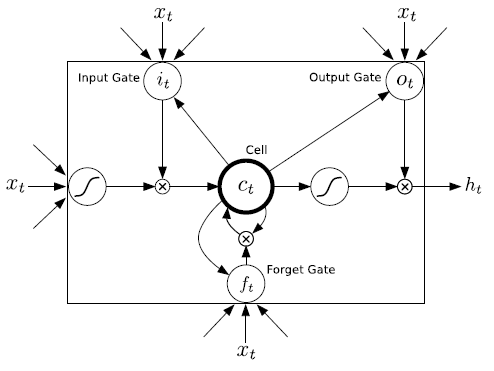
\includegraphics[width=7cm]{lstmcell}\\
  \caption{An LSTM Cell  \citep{graves2013hybrid}}\label{fig_3_3_lstmcell}
\end{figure}

The gates in the above formula are illustrated in Figure \ref{fig_3_3_lstmcell}.  $\mathbf{i}_t$ represents the input gate, $\mathbf{f}_t$ is the forget gate and $\mathbf{o}_t$ represents the output gate.  At each of these gates therefore, the inputs consisting of hidden states in addition to the regular inputs are multiplied by a set of weights and passed through a soft-max function. These weights during training learn whether the gate will, during inference, open or not.  In summary, the input gate tells the LSTM whether or not to receive new information, the forget gate determines whether the current information it already has from the previous step should be kept or dropped and the output gate determines what should be forwarded to the next LSTM cell.  Note also that the LSTM has two sigmoid ($tanh$) activation functions utilised at the input and output of the current cell $\mathbf{c}_t$.

One particular variant of the original LSTM model is the GRU cell. Though simpler than an LSTM cell the GRU cell performs equally efficiently.   The GRU cell is a subset implementation of the LSTM cell.  Rather than using the output gate of the LSTM, this gate is omitted in the GRU and the output result of the other internal gates are always forwarded.  The second simplification is a merge of the internal gate state vectors into a single vector $\mathbf{h}_{(t)}$.  This merged gate here referred to as $\mathbf{z}(t)$, controls both the forget gate an the input gate and acts as follows. Whenever a value is retained by the cell the previous value is erased first.  That is, if the gate controller outputs a 1, in the LSTM this corresponds to the input gate is open and the forget gate is closed. Therefore if $\mathbf{z}(t)$ it outputs a 0, the reverse happens for the input gate and the forget gate in the LSTM.  There is, however, a new gate controller, $\mathbf{r}(t)$, which determines which portion of the previous state will be shown at the output \citep{cho2014learning}.

The architecture of a GRU is formulated as follows:
\begin{equation}
\mathbf{z}_{(t)}=\sigma(\mathbf{W}_{xz}^T\cdot\mathbf{x}_{(t)}+\mathbf{W}_{hz}^T\cdot\mathbf{x}_{(t-1)})\label{eqn_c3_gru01}
\end{equation}
\begin{equation}
\mathbf{r}_{(t)}=\sigma(\mathbf{W}_{xr}^T\cdot\mathbf{x}_{(t)}+\mathbf{W}_{hr}^T\cdot\mathbf{x}_{(t-1)})\label{eqn_c3_gru01}
\end{equation}\begin{equation}
\mathbf{g}_{(t)}=\tanh(\mathbf{W}_{xg}^T\cdot\mathbf{x}_{(t)}+\mathbf{W}_{hg}^T\cdot(\mathbf{r}_{(t)}\otimes\mathbf{h}_{(t-1)}))\label{eqn_c3_gru01}
\end{equation}\begin{equation}
\mathbf{h}_{(t)}=(1-\mathbf{z}_{(t)})\otimes(\mathbf{h}_{(t-1)})+\mathbf{z}_{(t)}\otimes\mathbf{g}_{t}\label{eqn_c3_gru01}
\end{equation}

Due to the light-weight nature of the GRU cell, it is common practice to use GRU cells in place of LSTM cells.  This precedence achieves the much desired lighter computation load on the actual hardware performing the RNN training. As each of the gates required in an LSTM cell comprises high density matrix multiplication operations in themselves, the condensation of two gates into one and the omission of the output gate within GRU cells pushes towards halving the architectural complexity and coupled with the equally efficient performance of the GRU when compared to the LSTM cell ultimately serves as an overall improvement on the LSTM architecture.  For these reasons, GRUs have highly appealing features when compared to LSTMs and was the RNN cell of choice used for the study in this report.

\section{Deep speech architecture}\label{deepspeech}

This work makes use of an enhanced RNN architecture called the Bi-directional Recurrent Neural Network (BiRNN). While \cite{hannun2014first} assert that forward recurrent connections does reflect the sequential relationships of an audio waveform, perhaps the BiRNN model achieves a more robust sequence model.

The BiRNN is a preferred end to end mechanism due to the length of sequence over which temporal relationships can be captured.  This implies that BiRNNs will be suited for capturing temporal relationships over much longer sequences than a forward only RNN, because hidden state information is preserved in both forwards and backwards direction. 

In addition, such a model has a notion of complete sentence or utterance  integration, having information over the entire temporal extent of the input features when making each prediction. 

The formulation of the BiRNN is derived by starting off with the basic RNN architecture which is referred to as the forward architecture.  From the forward architecture we derive the backward architecture. If we choose a temporally recurrent layer $j$, the BiRNN forward and backward intermediate hidden representation $h^{(f)}_t$ and $h^{(b)}_t$ is given as. 
\begin{equation}h_t^{(f)}=\sigma(\mathbf{W}^{(j)T}h_t^{(i-1)}+\mathbf{W}^{(f)T}_kh_{t-1}^{(j)}+b^{(j)}))
\label{eqn_c3_ds01}\end{equation}
\begin{equation}h_t^{(b)}=\sigma(\mathbf{W}^{(j)T}h_t^{(i-1)}+\mathbf{W}^{(b)T}_kh_{t+1}^{(b)}+b^{(j)}))
\label{eqn_c3_ds02}\end{equation}

Temporal weight matrices $W^{(f)}$ and $W^{(b)}$ propagate $h^{(f)}_t$  and $h^{(b)}_t$ forward and backward in time respectively. 

\cite{hannun2014first} points out that the recurrent forward and backward components are evaluated entirely independent of each other and for optimal training, a modified non linearity function $\sigma(z) = min(max(z, 0), 20)$ is recommended. 

The final BiRNN representation $h^{(j)}_t$ for the layer is now the superposition of the two RNN components,
 \begin{equation}h_t^{(j)}=h_t^{(f)}+h_t^{(b)}
\label{eqn_c3_ds03}\end{equation}
Also note that back propagation through time (BPTT) sub gradient evaluations are computed from the combined BiRNN structure directly during training.

\subsection{Connectionist Temporal Classification (CTC)}\label{c3_ctc}
The term CTC stands for Connectionist Temporal classification.  This algorithm was designed to solve the problem of fuzzy alignment between the source input data and the output classification desired from the Machine Learning system.  This type of fuzzy alignment is observed in speech recognition systems since the same speech in either the same individual or different individuals will have different signal forms.  This is a many to one relationship between the input signal and the output classification that is also dependent on the style of speaking at the moment when the utterance is said.  Unlike hybrid DNN-HMM networks the CTC algorithm deploys an end-to-end framework that models all aspects of the input sequence in a single neural network, therefore discarding the need for an HMM interpretation of the input sequence. In  addition, the CTC method does not require pre-segmented training data at the same time output classification is made independent of post-processing.

CTC works by making predictions at any point in the input sequence. For the case of speech modelling,  CTC makes a character prediction for every time step of the raw audio input speech signal. Although this initially seems counter intuitive, this method models the many to one relationship seen in the fuzzy audio speech to text alignment. 

For hybrid DNN-HMM systems, speech or more accurately, acoustic models, require separate training of targets for every time-slice in the input sequence. Secondly, and  as a consequence of this, it becomes necessary to segment the audio sequence, in order to provide targets for every time-slice. A third consequence is the limitation of DNNs previously discussed. As the DNN network only outputs local classifications, global aspects such as the likelihood of two consecutive labels appearing together cannot be directly modelled.  Without an external model, usually in the form of a language model, the hybrid speech model will significantly degrade performance.

In the CTC case, so long as the overall sequence of labels is correct the network can be optimised to correct the temporal or fuzzy alignments. Since this many to one fuzzy alignment is simultaneously modelled in CTC, then there is no need for pre-segmented data. At the same time, CTC computes probabilities of complete label sequences, hence external post-processing required by hybrid models is eliminated.

Similar to the HMM sequence model, the CTC algorithm is a sequence model that predicts the next label in a sequence as a cumulative of previous sequences.  This section develops the CTC loss function borrowing concepts used in HMM models such as the forward backward algorithm as outlined in \citep{graves2006connectionist}.  In the following paragraph we introduce terminology associated with the CTC loss function.

Given two symbols $A$ and $\mathcal{B}$ such that $A$ has a many to one relationship with $\mathcal{B}$, signifying the temporal nature of the classification. The symbol $A$ represents an alphabet from which a sequence of the output classifications are drawn from. This CTC output consists of a soft-max layer in a BiRNN (bidirectional recurrent neural network). 

This output models the probability distribution of a complete sequence of arbitrary length $|A|$ over all possible labels in $A$ from activations within $|A|$. An extra activation is given to represent the probability of outputting a $blank$, or no label. At each time-step leading up to the final step, the probability distribution estimated as distribution over all possible label sequences of length leading up to that of the input sequence.

It is now possible to define the extended alphabet $A' = A \cup \{blank\}$, also, $y_{t,p}$ as the activation of network output $p$ at time $t$.  Therefore $y_{t,p}$  is the probability that the network will output element $p \in A'$ at time $t$ given that $x$ is the input sequence of length $T$.  The distribution sought after $Pr(\pi|x)$, is the conditionally-independent distribution over the subset $A'^T$ where $A'^T$ denotes the set of length $T$ sequences in $A'$. 
\begin{equation}
\Pr( \pi \, | \, x ) = \prod_{t=1}^{T} y_{t,\pi_t}
\label{eqn_c4_ctc01}\end{equation}

From Equation (\ref{eqn_c4_ctc01}), it is now possible to define the many-to-one mapping $\mathcal{B} : {A‘}^T \rightarrow A^{\le T}$.  This is the mapping of a set $A'^T$,  which indicates the paths, onto another set  $A^{\le T}$, that of possible labels in $x$.  $\mathcal{B}$ then becomes a sequence of symbols with length less than or equal to $T$ over $A$. Note that $\mathcal{B}$ is a set containing sequential symbols belonging to the set $A$ and not. $A'$ because there is no blank symbol in $\mathcal{B}$.  This is achieved when first take out all repeated labels and then take out all the blanks from the sequence $A'^T$. For instance,

\begin{equation}\begin{aligned}\mathcal{B}(a - ab-) &= aab \\ \mathcal{B}(-aa - -abb) &= aab.\end{aligned} \label{eqn_c3_ctc02}
\end{equation}

The mapping obtained by $\mathcal{B}$ is equivalent to when the output switches from not predicting a new symbol to predicting a symbol or from predicting one symbol to another symbol assuming this was also possible.  Intuitively, the probability of $\mathcal{B}$ which is the labelling of $l \in A^{\le T}$ being a many to one of $A‘^T$ is determined by summing over all the paths in $A'^T$ mapped onto it by $\mathcal{B}$.  Thus:
\begin{equation}
\Pr( l \, | \, x) = \sum_{\pi \in \mathcal{B}^{-1}(l)} \Pr( \pi \, | \, x)
\label{eqn_c3_ct03}\end{equation}
This mapping makes CTC robust to unsegmented data as it predicts all the labels where they occur and later the ‘collapsed’ sequence will be extended over the approximate period where the previous extended sequence occurred thus aligning labels to input sequences on-the-fly without knowing in advance where label to input sequence alignments occur.

\subsection{Forward-backward algorithm}

The forward-backward algorithm is used to estimate the probability of a point in the sequence as the product of all point leading up to that point from the  initial state, the forward variable ($\alpha$), multiplied by the probability of all the points from that state to the end of the sequence, the backward variable ($\beta$).

The difference between this estimation and that determined from equation (\ref{eqn_c3_ct03}) is the fact that the forward-backward algorithm converts equation (\ref{eqn_c3_ct03}) into a form that is both recursive as well as reduces the computational complexity from an otherwise intractable computation to one that is readily computable.

With CTC, consider a modified ``label sequence" $l'$, that caters for blank characters in between regular ones $l$, as defined in $A$. Thus, if $U$ is defined as the length of $l$.  Then $U'$ is of length $2U + 1$. CTC therefore integrates probability distributions of transitions between blank and non-blank labels at the same time CTC calculates those transition occurring between pairs of distinct non-blank labels.  The forward variable, $\alpha(t,u)$ now becomes the summed probability of all length $t$ paths that are mapped by $\mathcal{B}$ onto the length $\left \lfloor{u/2}\right \rfloor$ prefix of $l$. (Note, $\left \lfloor{u/2}\right \rfloor$ is the floor of $u/2$, the greatest integer less than or equal to $u/2$.) For some sequence $s$, let $s_{p:q}$ denote the sub-sequence $s_p, s_{p+1},\dots,s_{q-1},s_q$, and define the set $V(t,u) \equiv \{ \pi \in A'^t : \mathcal{B}(\pi) = l_{1:\left \lfloor{u/2}\right \rfloor} \text{ and } \pi_t = l'_u \}$.  $\alpha(t,u)$ then becomes
\begin{equation}
\alpha(t,u) \equiv \sum_{\pi \in V(t,u)} \prod_{i=1}^{t} y_{i,\pi_i} 
\label{eqn_c3_ctc04}
\end{equation}

The forward variables at time $t$ is calculated recursively from the preceding values at time $t - 1$ and expressed as the sum of the forward variables with and without the final blank at time $T$.

\begin{equation}
\Pr( l \, | \, x) = \alpha(T, U') + \alpha(T, U' - 1)
\label{eqn_c3_ctc05}
\end{equation}

For the initial conditions, correct paths begin with a blank symbol $(b)$ and the first symbol $l$ $(l_1)$:
\begin{equation}
\begin{aligned}\alpha(1, 1) &= y_{1,b} \\ \alpha(1, 2) &= y_{1,l_1} \\ \alpha(1, u) &= 0, \, \forall u > 2 \end{aligned}
\label{eqn_c3_ctc05}\end{equation}

The forward variable then takes the following recursive form:
\begin{equation}
\alpha(t,u) = y_{t, l'_u} \sum_{i = f(u)}^{u} \alpha(t-1, i)
\label{eqn_c3_ctc06}\end{equation}
where
\begin{equation}
f(u) =\begin{cases}u-1, & \text{ if } l'_u = blank \text{ or } l'_{u-2} = l'_{u} \\ u-2, & \text{otherwise}\end{cases}
\label{eqn_c3_ctc07}
\end{equation}

Figure \ref{fig_c4_lattice} expresses the recurrence relation for $\alpha(t, u)$. While $t$ is expressed on the $x$ axis, $u$ is illustrated on the $y$ axis. The CTC algorithm assumes that outputs of the network potentially alternate between blank symbols indicated as black circles  and non-blank elements, the white circles, all in $l'$.  The sequential graph constructed from this 2-dimensional matrix show computational dependencies between sequential pairs of the recurrence relation for $\alpha(t,u)$. Therefore, the value $\alpha(2,3)$, formed from $\alpha(1,2)$, corresponds to the $blank$ symbol at $t=2$ and $u=3$, is . Also,  $\alpha(2,2)$, equivalent to the symbol $c$ at $t=2$ and $u=2$, is gotten from $\alpha(1,2)$ and $\alpha(1,1)$.  Note that there are not enough time steps when $u < U'−2(T−t)−1$, therefore, $\alpha(t,u)=0$. 

\begin{figure}
\centering
  % Requires \usepackage{graphicx}
  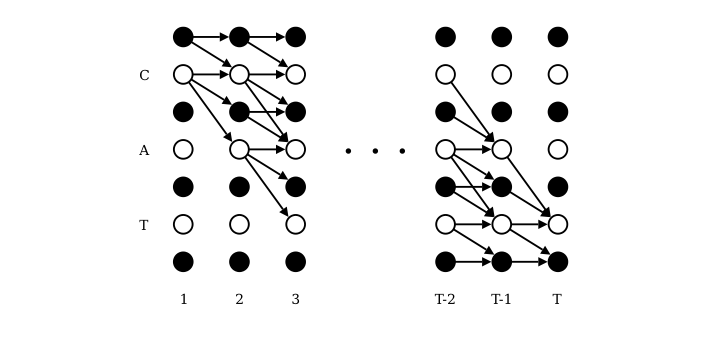
\includegraphics[width=9cm]{thesis/images/Lattice.png}
  \caption{Beam Search Lattice Structure \citep{graves2006connectionist}}
\label{fig_c4_lattice}
\end{figure}

Also note the boundary condition;
\begin{equation}
\alpha(t, 0) = 0 \quad \forall t
\label{eqn_c3_ctc08}
\end{equation}
The backward variable $\beta(t,u)$ ais built similarly to the forward variable. Rather than moving from the start of the sequence to  we define the path starting at $t + 1$ that completes the sequence at $T$ when appended to any path $\hat{\pi}$ that generates $\alpha(t,u)$. Then, assuming $W(t,u) \equiv \{ \pi \in A'^{T-t} : \mathcal{B}(\hat{\pi} + \pi) = l \, \, \forall \hat{\pi} \in V(t,u) \}$, therefore
\begin{equation}
\beta(t,u) \equiv \sum_{\pi \in W(t,u)} \prod_{i=1}^{T - t} y_{t + i,\pi_i} \label{eqn_c3_ctc08}\end{equation}

The backward variable is therefore equivalently initialised as thus

\begin{equation} \begin{aligned}
\beta(T, U') &= 1 \\
\beta(T, U' - 1) &= 1 \\
\beta(T, u) &= 0, \, \forall u < U' - 1
\end{aligned}\label{eqn_c3_ctc09}\end{equation}

The recursion rule is defined as follows:
\begin{equation}
\beta(t, u) = \sum_{i = u}^{g(u)} \beta(t+1, i) y_{t+1, l'_i}\label{eqn_c3_ctc10}\end{equation}
similarly,
\begin{equation}
g(u) = \begin{cases} u + 1,& \text{if } l'_u = blank \text{ or } l'_{u+2} = l'_{u} \\ u + 2,& \text{otherwise} \end{cases}   
\end{equation}

\subsection{CTC Loss function}\label{sec_c4_ctcloss}

The cross entropy error is a loss function used to measure accuracy of probabilistic measures.  It is calculated as the negative log probability of a likelihood measure.  The CTC loss function $\mathcal{L}(S)$ uses the cross entropy loss function of and is defined as the cross entropy error of correctly labelling all the training samples in some training set S:
\begin{equation}
\mathcal{L}(S) = - \ln \prod_{(x,z) \in S} \Pr(z \, | \, x) = - \sum_{(x,z) \in S} \ln \Pr(z \, | \, x)
\label{eqn_c3_ctc11}\end{equation}
where $z$ is the output label and $x$ is the input sequence.  Since $\mathcal{L}(S)$ in equation \ref{eqn_c3_ctc11} is differentiable, this loss function can be back propagated to the softmax layer in the BiRNN configuration discussed in section \ref{deepspeech}.
\begin{equation}
\mathcal{L}(x,z) \equiv - \ln \Pr(z \, | \, x)
\label{eqn_c3_ctc12}\end{equation}
and therefore 
\begin{equation}
\mathcal{L}(S) = \sum_{(x,z) \in S} \mathcal{L}(x,z)
\label{eqn_c3_ctc12}\end{equation}

From the definition of the forward and backward variables ($\alpha(t, u)$ and $\beta(t, u)$), we also establish that $X(t,u) \equiv \{ \pi \in A'^T : \mathcal{B}(\pi) = z, \, \pi_t = z'_u \}$, such that
\begin{equation}
\alpha(t, u) \beta(t, u) = \sum_{\pi \in X(t,u)} \prod_{t = 1}^{T} y_{t, \pi_t}\label{eqn_c3_ctc13}\end{equation}

then substituting $\Pr(\pi \, | \, x)$ from the expression in equation \ref{eqn_c3_ctc01}, we have
\begin{equation}
\alpha(t, u) \beta(t, u) = \sum_{\pi \in X(t,u)} \Pr(\pi \, | \, x)
\label{eqn_c3_ctc14}\end{equation}

Also observe that $\Pr(l \, | \, x)$ is equivalent to the total probability $\Pr(z \, | \, x)$. Paths going through $z'_u$ at time $t$ can be obtained as summed over all $u$ to get
\begin{equation}
\Pr(z \, | \, x) = \sum_{u = 1}^{|z'|} \alpha(t, u) \beta(t, u)
\label{eqn_c3_ctc15}\end{equation}

Thus a sample loss is determined by
\begin{equation}
\mathcal{L}(x, z) = - \ln \sum_{u = 1}^{|z'|} \alpha(t, u) \beta(t, u)\label{eqn_c3_ctc16}
\end{equation}
and therefore the overall loss is given by
\begin{equation}\mathcal{L}(S) = -\sum_{(x,z) \in S} \ln \sum_{u = 1}^{|z'|} \alpha(t, u) \beta(t, u)
\label{eqn_c3_ctc17}\end{equation}

In the model described in this work, the gradient $\mathcal{L}(x, z)$is computed using TensorFlow's automatic differentiation capabilities. In practice, computations soon lead to underflow.  However, the log scale, being used in the above loss function calculations avoids this situation and another useful equation in this context is
\begin{equation}
\ln(a + b) = \ln(a) + \ln(1 + e^{\ln b - \ln a})
\label{eqn_c3_ctc18}\end{equation}


\startblue
\section{Attention Mechanism}\label{sec_45_attn}

This can be likened to how neural networks simulate how the human brain functions in achieving tasks.   Attention is a cognitive process of concentrating on one or a few things and at the same time ignoring others.  Therefore attention mechanism focuses more on the informative data segment of a model that contributes more to the final output.  It creates an underlying relationship between the input and output of a model producing improved transduction from input to output sequence. 

Attention mechanism is an extension to the sequence-to-sequence asynchronous \acrshort{mimo} \acrshort{rnn} architecture discussed in Section \ref{sec_postalign}.  The objective of attention-based networks highlighted by \cite{vaswani2017attention} is to reduce sequential computation while attaining hidden representation across arbitrary lengths of sequential input. Some other strategies which have also attempted to achieve this includes a combination of convolutional and recurrent schemes \citep{kaiser2016can,kalchbrenner2016neural, gehring2017convolutional}.

\begin{figure}
\centering
  % Requires \usepackage{graphicx}
  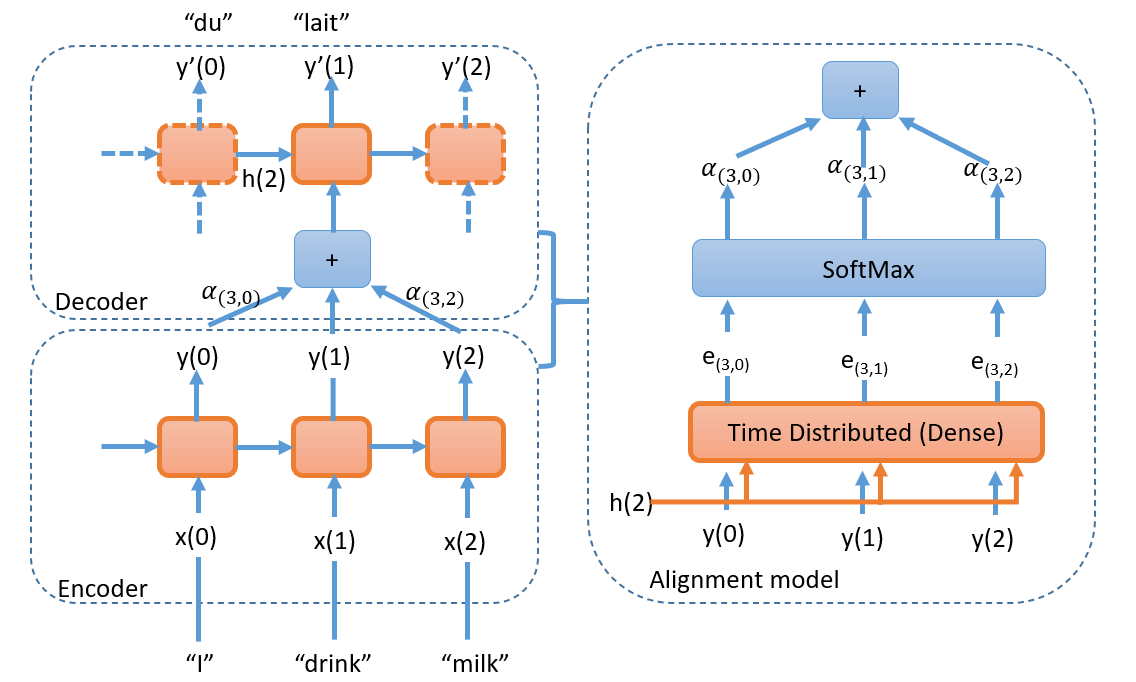
\includegraphics[width=12cm]{thesis/images/attention.PNG}
  \caption{Attention mechanism}
\label{fig_c4_attn}
\end{figure}

Attention is achieved by joint training of an attention neuron that takes outputs of the hidden layer of each input in the encoder along with the entire \acrshort{rnn} as shown in figure \ref{fig_c4_attn}.  In the original attention mechanism proposed by \cite{bahdanau2014neural}, the weighted sum of all encoder outputs will determine what segment of the sequence receives more attention.  The output of this attention neuron at each time-step is then concatenated with the output of the \acrshort{rnn} and fed to the decoder.

Since dot product is a fairly decent measure of similarity, and faster to compute,\cite{luong2015effective} proposed a dot product between encoder’s output and decoder’s previous hidden state as a basis for attention mechanism.  For this to work however, both of these vectors must be of the same dimensions.  This type of attention mechanism is known as multiplicative attention.  Just like in Concatenative attention, the dot product gives a score and all the scores (at a given decoder timestep) go through a softmax layer to give the final weights.  

In equation \ref{eqn_c4_attn00} below, $\mathbf{\tilde{h}}_{(t)}$, is the output of the attention neurons and $\alpha_{(t,i)}$ represents the weight of each output that is jointly learned where $e_{(t,i)}$ represents variants of how the weights can be obtained.  Here three variants are shown either dot, general or concatenation. The dot and general are variants proposed by \cite{luong2015effective}.  The general proposition represents $e_{(t,i)}$ as the dot product of decoder hidden weights with the linear transposition of the encoder outputs (i.e. time-distributed Dense layer with no bias term).  Another modification proposed was to use the decoder’s hidden state at the current time step rather than at the previous time step (i.e., $\mathbf{h}_{(t)}$ rather than, $\mathbf{h}_{(t-1)}$), then use the output from the attention mechanism ( $\mathbf{\tilde{h}}_{(t)}$) directly to compute the decoder's predictions (rather than using it to compute the decoder’s current hidden state).  They also discovered that by adding a re scaling parameter $\mathbf{v}$, to the concatenative attention mechanism these three dot product variants perform better than the simple concatenative attention.

\begin{equation} \begin{aligned}
\mathbf{\tilde{h}}_{(t)} &= \sum_i\alpha_{(t,i)}\mathbf{y}_{(i)} \\
\text{with }\alpha_{(t,i)} &= \frac{exp(e_{(t,i)})}{\sum_{i'}exp(e_{(t,i')})} \\
\text{and } &= \begin{cases} \mathbf{h}_{(t)}^\top\mathbf{y}_{(i)} & dot\\ 
\mathbf{h}_{(t)}^\top\mathbf{W}\mathbf{y}_{(i)} &  general \\
\mathbf{v}^\top\tanh{(\mathbf{W}[\mathbf{h}_{(t)};\mathbf{y}_{(i)}]) & concatenate
\end{cases} 
\end{aligned}\label{eqn_c4_attn00}\end{equation}

\cite{vaswani2017attention} introduces a transduction model known as a Transformer based on self attention network with the ability to compute long term dependencies while eliminating sequence aligned RNN and convolutional architectures.  Although this study makes use of \acrshort{rnn} transducers with attention, integration of the self-attention architecture was left for a further study.
\stopblue

\section{Chapter Summary}
Deep Neural Networks (DNNs) are at the centre of the models developed within this research.  They are able to overcome the challenge of complex modelling of latent information when discriminating directly from the data.  To this extent, they tend to be data intensive in nature.  In this chapter, neural network architectures and algorithms were considered.  The Chapter begins with the rudimentary Perceptron algorithm which is the precursor to the logistic regression algorithm.  The Neural Network and \acrfull{mlp}, uses logistic regression concept and adds an extra layer of neurons and back propagation algorithm to optimise classifications.  

The Deep Neural Networks used within this research are special DNNs which are able to identify patterns in data having sequential patterns.  These are the deep Recurrent Neural Networks (RNNs).  It is shown in this Chapter that RNNs are able to learn the recurrent relationship information by modifying their architecture such that the data paths among the neurons are modified so that hidden states are also used as inputs.  In addition the back propagation algorithm is also modified in terms of datapaths of the algorithm output to reflect the sequential structure of the neural network.

Special categories of RNNs used to build speech and language models developed in this thesis are the Long Short-Term Memory (LSTM) and Gated Recurrent Unit (GRU) RNN cells.  In this research were utilised for development of a character-based language model and the Bidirectional RNN (Bi-RNN) used for development of the speech model.  

A special algorithm, the Connectionist Temporal Classification (CTC) algorithm, also employed by the BiRNN is described in this Chapter.  The CTC algorithm overcomes the challenge of a character-based speech model when considering misaligned nature of audio data between specific points in the audio that correspond to equivalent characters in the transcription.   In addition, it is also discussed how the CTC algorithm utilises the forward-backward algorithm to perform classification.  In a later Chapter \ref{ch6_speech}, the prefix beam search algorithm is described, and, in combination with output probabilities obtained from the CTC algorithm and a language model, performs decoding of the output into the actual speech-to-text translations.


\chapter{Deep Scattering network}\label{ch4DSN}
A language model for the Wakirike language is developed in this chapter.  This model draws upon the premise that the grammar of a language is expressed in the character sequence pattern which is ultimately expressed in words and therefore the abstract grammar rules can be extracted and learned by a character-based RNN neural network.

\section{Data Preparation}
The Wakirike New Testament Bible served as the source of data for the deep neural network training.  As there wasn't a readily available soft or on-line copy of the Wakirike new testament bible for use, this was typed, giving rise to a complete corpus word size of 668,522 words and a character count of 6,539,176 characters. The dataset was then divided into 11 parts. Two parts dedicated for testing and validation and the remaining 9 parts were used for training.

The Unicode representations of the character set consisting of letters and punctuation marks are one-hot encoded and batched for sequential input, each batch having a character sequence length of 30 characters.


\section{GRU Training}.

The modified LSTM RNN known as the Gated Recurrent Unit (GRU) is employed for the neural network model in order to optimise network performance in terms of resource conservation.  GRUs have been shown to give similar performance to regular LSTMs however, with a lighter system resource footprint \citep{cho2014learning}. The GRU RNN used to train the Wakirike text corpus comprised an internal network size of 512 nodes for each layer and was 3 layers deep. Externally, 30 GRUs represented  the number of recurrent connections each connection representing a time step bearing contextual for the recurrent input sequence. 

To mitigate for overfitting, due to the multi-layered high-dimensional depth of this neural network, a small learning rate of 0.001 was used. To further marginalise overfitting the popular and effective dropout \citep{srivastava2014dropout} method for regularising deep neural networks kept at 20\% such that only 80\% activations were propagated from one layer to the next and the remaining 20\% were zeroed out.

\subsection{Output Language Generation}
The neural network is trained for 10 epochs and achieves a prediction accuracy of 85\% on held-out data.  With the GRU model it is possible to seed this network with an input character and select from the top-N candidates thus causing the Neural network to generate its own sentences.  In this scenario, the network is said to perform language generation by immanently constructing its own sentences.  The generated language was found to be intelligibly similar to that of the training data. 

A clever use of this new corpus generated by the GRU language model of this work was to determine a word-based perplexity metric for the GRU neural language model. In this work, the word-based perplexity metric was achieved from the output language generated by first estimating the word based perplexity on the training data.  The same perplexity calculation was then used on the generated neural language model corpus. The corpus size of the neural language model was made to be equivalent to that of the training data, that is containing 6,539,176 characters.  The perplexity calculation was based on a modified Kneser-Key 5-gram model with smoothing (Ref).  The results discussed below showed that the LSTM model generated a superior model compared to the n-gram model that better matched the training data.

The evaluation of the GRU language model of the Wakirike language was performed using a perplexity measurement metric. The Perplexity metric applies the language model to a test dataset and measures how probable the test dataset is. Perplexity is a relative measure given by the formula:


\begin{table}
  \caption{Perplexity Calculation results}
  \label{tab:example}
\begin{tabular}{lr}
\toprule
Language Model & Perplexity\\
\midrule
LSTM RNN & 2.6\\
3-gram with Keysner Soothing and interpolation & 3.3\\
\bottomrule
\end{tabular}
\end{table}


The result of the training of the Long-short-term-memory (LSTM)-Cell Recurrent Neural Network on low-resourced Wakirike Language gave impressive and intelligible results and showed better results when measured with standard n-gram language models. The results showed that it is indeed possible to use an LSTM on a low resource character sequence corpus to produce an Wakirike language model.

The evaluation of the LSTM language model of the Wakirike language was performed using a perplexity measurement metric. The Perplexity metric applies the language model to a test dataset and measures how probable the test dataset is. Perplexity is a relative measure given by the formula:

%
\begin{equation}
PP(W)=P(w_1,w_2\dots w_N)^\frac{1}{N}
\label{eq6}
\end{equation}
%
%
\begin{equation}
PP(W)=\sqrt[N]{\prod_{i=1}^N\frac{1}{P(w_i|w_{i-1})}}
\label{eq7}
\end{equation}
%

Where $w_1,\dots,w_N$ are the sequence of words. The language model with the lower relative perplexity score is therefore expected to yield better approximation of the data when applied to unseen data generally.

There was no way however to directly measure perplexity on a character sequence model because perplexity is usually used to evaluate word-based models.  However, this limitation was overcome by performing n-gram analysis on the corpus entirely generated from the LSTM network. The generated n-gram model from the generated corpus is then applied to test data and the perplexity is measured.

Table ~\ref{tab:example} below shows the Results of the Perplexity model of the LSTM Wakirike Language model and an equivalent Trigram Language model with interpolation and Keysner smoothing \cite{chen1996empirical}.
Table 1 below shows the Results of the Perplexity model of the LSTM Wakirike Language model and an equivalent Tri-gram Language model with interpolation and Keysner smoothing.

It can be inferred that the LSTM character-model developed has an improved language model and because it is based on a character-model, which is fine-grained when compared to a word model, it is likely to generalise data better when used in practice is and less biased than a word-based model.  This can be observed from the fact that the output corpus produced a larger vocabulary size.


\chapter{Wakirike Language Model}\label{ch6_wlm}

\textcolor{blue}{
The details of the language models developed for the Wakirike language is discussed in this chapter.  The language models developed draw  upon the premise that the grammar of a language is expressed in the character sequence pattern ultimately rendered in word sequences.  The two models developed in this chapter follow RNN implementations discussed in chapter \ref{ch3RNN}. }

\section{Data Preparation}
\startblue
A published version of the Wakirike New Testament Bible was obtained and used as the data source for RNN training of the language model.  There was no readily available soft or on-line copy of the Wakirike new testament bible. As such, the Wakirike New Testament Bible text corpus text was entered into the ASR system from the physical copy using a text editor to form a text corpus.  The complete corpus had a word count of 668,522 words and a character count of 6,539,176 characters. Following the k-fold cross validation process, \citep{geron2019hands}, the data set was then divided into 11 parts. Two parts dedicated for testing and validation and the remaining nine parts were used for training. As the validation set is not seen during training it can be used to keep track of how well the training is going and that it is not over-fitting the data by simply memorising it.

Preprocessing of the text corpus involved selecting a set of characters as the input feature set and removing all other characters not found in the input feature set.  The Unicode representations of the character set consisted of letters and punctuation marks.  These are one-hot encoded and batched for sequential input.  Neural network parameters which are not automatically determined through back propagation are called hyper-parameters.  These are usually experimentally determined and manually set while configuring the network.  A hyper-parameter for the language model RNN is the input sequence length.  For the language model built a 30 characters-long sequence length is chosen.  This  length is an average phrase sequence.  In these phrases, long-term character dependencies of words can be captured. At the same time, keeping the sequence length at this value, and not longer, will pose less of a burden on the computer system resources during parameter computations.  

Another hyper-parameter for training used was the batch size.  The batch size parameter determined how many 30-character sequences will be trained in parallel in order to speed up the training process.  Increasing the batch size also meant an increase in the size of the matrix multiplications being performed and therefore, the computing power system resource being demanded by the language model.  By experimenting with various batch sizes it was determined a batch size of 200 was suitable for training the language model with respect to the other training parameters.

\section{GRU RNN Architecture}
The modified LSTM RNN known as the Gated Recurrent Unit (GRU) discussed in Chapter \ref{ch3RNN} is employed for the neural network model built in this Chapter.  In order to optimise network performance while conserving computation resources, GRUs have been shown to give similar performance to regular LSTMs however, with a lighter system resource footprint \citep{cho2014learning}. 

The architecture of the GRU RNN used to train the Wakirike text corpus had an internal network size of 512 nodes for each layer and was 3 layers deep. In a study by \citep{goodfellow2013multi}, it was shown that increasing the number of nodes in a neural network will lead to over-fitting, however, simultaneously increasing the network depth mitigates this effect.  In other words, in order to expand the degrees of freedom of a neural network and at the same time constrain the network to generalise well on unseen data, it is necessary to increase the number of neurons in both length and depth.  Experiments carried out in this chapter follow this recommendation. Initial experiments had an internal node size of 128 and a single layer deep.  While this showed promise of converging, the error rate was still high, therefore the network was expanded to the final model above.   Externally, the network model is further  sequenced 30 times, representing the input sequence length hyper-parameter and the number of recurrent connections where each connection represents a sequenced time step. 

Another hyper-parameter sensitive to network size is the learning rate.  The learning rate is selected in such a manner that an increase in the network size makes the learning rate more prone to overshooting.  Therefore, increased degrees of freedom in a neural network will require the learning rate to be made smaller so that it does not overshoot the network saturation point.  Small learning rates of between 0.001 and 0.005 were used. Furthermore, the language model neural network was designed to overcome over-fitting using the dropout method \citep{srivastava2014dropout} which has been shown to be effective for regularising deep neural networks.  The hyper-parameter for dropout was kept at 20\% such that only 80\% of neural network activations are propagated from one layer to the next, whereas the remaining 20\% were randomly zeroed out.  Intuitively, dropout works by forcing the remaining active neurons to infer what is missing in the activations that have been dropped and ultimately leads to better generalisations as activations are based on inference than on memory.

\section{Language Model Training Experiments}
Two sets of character-based neural network RNN-based experiments are developed in this chapter.  A third word based statistically modelled language model is also developed based on  \cite{Heafield-estimate} estimates as a baseline model. Character-based perplexity measurements were used to compare the character-based models and a conversion factor based on \citep{hwang2017character} is used to compare character-based models on the word-based counterparts.  Experiments for the RNN language models were majorly performed using tensorflow-MKL, which is a highly parallelised (44-threads for one of the experiments) cpu-based experiments.  The experiment with the largest number of neurons was also performed on cloud-based GPUs (Nvida Tesla T4).  Details of the experiments carried out and resulting perplexity are shown in Table \ref{tab6_1:LMX}.

\begin{table}
  \caption{Language Models comparison}
  \label{tab6_1:LMX}
\begin{tabular}{lrrr}
\toprule
Language Model & Train time & Perplexity & Epochs  \\
\midrule
GRU RNN 3-layer model (CPU training) & ~ 2 days & 30.920 & 75 \\
5-gram with Keysner Soothing and interpolation & 5 minutes & 238.720 & N/A \\
GRU RNN single-layer model (GPU training) & ~ 5 hours & $2.35\times10^{13}$ & 120 \\
GRU RNN 3-layer model (cloud GPU training) & ~ 2 hours & 30.920 & 75 \\
\bottomrule
\end{tabular}
\end{table}

\stopblue


\section{Output Language Model and Language Generation}
\startblue
The 3-layer network experiments were trained on both CPU and GPU configurations. Both were trained for 75 epochs, where an epoch indicates that the model has processed all of the training data.  Recall that the model  is trained until it is saturated.  In other words, the model trains until the prediction accuracy is no longer improving.   This usually will take several epochs.

The loss plots for the three-layer and single layer GRU RNN are shown in Figure \ref{fig_ch7_00losses}.  The three-layer GRU-RNN achieved a prediction accuracy of 65\% on held-out data.  When the created 3-layer GRU character-based RNN language model is seeded with an input character, one can force the network to select from the top-N candidates thus causing the Neural network to generate its own sentences.  In this scenario, the network is said to perform language generation by constructing its own sentences.  The generated language output from the GRU language model was found to be a reflection of the overall context of the training data. 

\begin{figure}
\centering
  % Requires \usepackage{graphicx}
  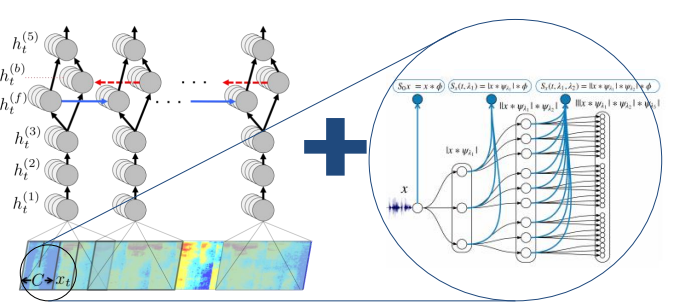
\includegraphics[width=14cm]{thesis/images/ctc_scatter.png}\\
  \caption{Deep scattering Bi-RNN Model} \label{fig_ch7_00losses}
\end{figure}

The evaluation of the GRU language model of the Wakirike language was performed using a perplexity measurement metric. The Perplexity metric applies the language model to a test data-set and measures how probable the test data-set is. Perplexity is a relative measure given by the formula:
%
\begin{equation}
PP(W)=P(w_1,w_2\dots w_N)^\frac{1}{N}
\label{ch5_eq1_ppx}
\end{equation}
%
%
\begin{equation}
PP(W)=\sqrt[N]{\prod_{i=1}^N\frac{1}{P(w_i|w_{i-1})}}
\label{ch5_eq2_ppx}
\end{equation}
%
Where $w_1,\dots,w_N$ are the sequence of words. The language model with the lower relative perplexity score is therefore expected to yield better approximation of the data when applied to unseen data generally.

The result of the training of the GRU-Cell Recurrent Neural Network on low-resourced Wakirike Language gave impressive and intelligible results and showed better results when measured with standard n-gram language models. The results showed that it is indeed possible to derive a language model using a GRU-cell RNN on a low resource character sequence corpus for the Wakirike language.

A character based perplexity metric is possible using  the negative log likelihood of the character sequence.
\begin{equation}
    PP(X)=exp\left\{−\frac{\sum_{t=1}^T\log P(x_t|x_{1:t−1})}{T}\right\}
\label{ch5_eq3_ppx}
\end{equation}

However, our base-line language model is a 5-gram word-based language model.  Therefore, comparing a word based model to a character based model requires a conversion step. In this work, the conversion step involved using the GRU language model generated a corpus which was rescored by re-estimating with a 5-gram word-based language model

Table ~\ref{tab:example} shows the Results of the Perplexity model of the LSTM Wakirike Language model and an equivalent 5-gram Language model with interpolation and Keysner smoothing \citep{Heafield-estimate} for various lengths of the held-out data.
\stopblue

\section{Chapter Summary}
This chapter shows the application of a character-based Gated Recurrent Unit RNN on the low resource language of Wakirike to generate a language model for the Wakirike language.  The data-set and preparation and the details of the network were discussed.  The output of this model was used to hallucinate the Wakirike language which was then scored against word-based perplexity to obtain a metric against the baseline language model.

It can be inferred that the GRU character-model developed has an improved language model and because it is based on a character-model, which is fine-grained when compared to a word model, it is likely to generalise data better when used in practice and is less biased than a word-based model.  This can be observed from the fact that the output corpus produced a larger vocabulary size.


\chapter{Deep Recurrent Speech Recognition models}\label{ch6_speech}
\startblue
Throughout the development of this thesis, the establishment of deep learning as a strategy where computers learn through representation of patterns at varying degrees of complexity has been an underlying theme.  It was also emphasised how this is achieved by internal layer-wise encapsulations. Structures discussed in Chapter \ref{ch2litrev}, such as layer-wise stacking of neural network type architectures such as the \acrfull{rbm} and \acrfull{dbn} were used to implement such representations.  

In this chapter, the end-to-end Bi-directional Recurrent Neural Network model is described.  \acrshort{birnn} for speech recognition tasks is  employed here as opposed to regular \acrshort{rnn}s or \acrshort{dbn}s mentioned above in the preceding paragraph.  \acrshort{birnn}s are used because of the contextual nature of speech.  In Chapter \ref{ch6_wlm} it was demonstrated  how deep stacking of \acrshort{gru}s outperform single-layer \acrshort{rnn}s for extended sequences. That is to say, words in a sentence or paragraph are contextual to the sentence/paragraph over particularly long sequences and, these word contexts are better captured by the GRU architecture.  More importantly, \acrshort{birnn}'s have a forward and backward \acrshort{rnn} and these give the neural network the ability to analyse (look-up) the words from the backward RNN not currently seen by the forward RNN in the sentence succinctly giving the BiRNN parameters a contextual feature \citep{graves2006connectionist}.  

In addition to the procedure for designing sequence-to-sequence \acrshort{rnn}s outlined in Section \ref{sec_341_rnnproc}, this Chapter describes the training data, data preprocessing, derivation of feature vectors and output decoding.  First, speech features developed by making use of the deep scattering convolution networks \acrshort{dsn} is discussed.   The \acrshort{dsn}s are used as inputs to the end-to-end model.  Two end-to-end networks are then described.  The core \acrshort{birnn} network and a second \acrshort{birnn} network augmented with an RNN-transducer and an attention mechanism. A formal presentation of the speech neural network model parameters and architecture is given and the decoding algorithm is also detailed in sections contained within this chapter.  Finally, the results are presented and the findings from the model results discussed.\stopblue

\section{Deep Scattering Features}\label{sec_c7_wparams}
\textcolor{blue}{In Chapter 4, we derived a fast wavelet transform from a low pass filter and a high pass filter.  The speech features used for the BiRNN is obtained from successive wavelet-modulus operations of a deep scattering network 2 layers deep.  This 2-layer \acrshort{dsn} comprises a first-order scatter transform. The wavelet modulus operator is derived from the combination of a low pass filter and a band pass filter}.  Hyper parameters of the system included the window period for each sampled sub section, $T$;  The Q-band value for the band pass filter and the number of wavelets $J$ at each scattering layer for the total number of layers, $M=2$.

The matlab scatnet toolbox \citep{anden2014scatnet}, used to determine the scatter coefficient features for this research, provides optimal values for hyper parameters for audio signal processing into scatter features.  In this regime the value for the hyper parameter $T=512$ samples per window. This corresponds to a window of $50$ milliseconds for the audio signals sampled at $8000 Hz$.  For the first scattering layer the $Q$-band parameter was $Q=8$ and the second scattering layer took the value  $Q=1$.  Finally $J$ is pre-calculated based on the value of $T$.  These after Scat-Net processing produce a feature-vector having \textcolor{red}{$165$}  dimensions.  These feature vectors in turn are used as inputs to the bi-direction neural network model whose architecture is described in  succeeding sections.

\textcolor{blue}{For the second end-to-end architecture involving a transducer with attention mechanism, a period of  is used to capture a window of 4 seconds for audio signals sampled at 16000Hz. The same Q-band parameters having Q=8 for the zeroth layer and Q=1 for successive layers are used, In addition, the total number of layers deep was M=3 giving rise to a 2nd-order Scatter Network. This produced a feature-vector having 250 dimensions.}

\section{CTC-BiRNN Architecture}
The core of the system is a bidirectional recurrent neural network (BiRNN) trained to ingest scatter coefficients described in the previous section, in order to generate English text transcriptions.  An end-to-end system therefore specifies that utterances $x$ and the corresponding label $y$ be sampled from a training set such that the sample $S = {(x^{(1)}, y^{(1)}), (x^{(2)}, y^{(2)}), . . .}$.   In our end-to-end model, each utterance, $x^{(i)}$ is a processed feature vector consisting of $165$ dimensions.  Recall, every window passes through a scattering transform to yield an input of vector of $p=165$ features; consequently,   $x^{(i)}_{t,p}$ denotes the $p$-th feature in a scatter transform at time $t$.  

GPU training of the speech model architecture developed above was conducted using Mozilla deepspeech \citep{ardila2019common} CTC bi-directional RNN implementation along with the accompanying Mozilla Common voice dataset  \citep{mozilla_2019}.  The Common Voice Data set project consists of voice samples in short recordings approximately $4$ seconds each.  The complete dataset is about $250$ hours of recording divided into training, test and development subsets.  The BiRNN, given the input sequence, $x$, outputs a sequence of probabilities $y_t=\mathbb{P}(c_t|x)$,  where $c_t \in a,b,c,\dots,z,space,apostrophe,blank$. 

The actual architecture of our core Bi-RNN is similar to the deepspeech system described in \cite{hannun2014deep}. This structure constitutes 5 hidden layers and one output layer.  The first three layers are regular DNNs followed by a bi-directional recurrent layer. As such, the output of the first three layers are computed by:
\begin{equation}
    h^{(l)}_t = g(W^{(l)} h^{(l−1)}_t + b^{(l)})\label{ch06_01_l1-3}
\end{equation}

$g(\cdot) = min\{max\{0,z\},20\}$  is the clipped rectified linear unit and $W^{(l)},b^{(l)}$ are weight matrix and bias parameters for layer  as described in sections \ref{dnn} and \ref{deepspeech} respectively.

It was shown in chapter \ref{ch3RNN} the recurrent layer comprise a forward and backward RNNs whose equations are repeated here for reference
\begin{equation}
    h^{(f)}_t = g(W^{(4)} h^{(3)}_t + W^{(f)}_r h^{(f)}_{t−1} + b^{(4)})
    \label{ch06_02_fwd}
\end{equation}
\begin{equation}
h^{(b)}_t = g(W^{(4)} h^{(3)}_t + W^{(b)}_r h^{(b)}_{t+1} + b^{(4)})    \label{ch06_03_bwd}
\end{equation}

Consequently, $h^{(f)}$ is the sequential computation from $t=1$ to $t=T^{(i)}$ for the $i$-th utterance and $h^{(b)}$ is the reverse computation from $t=T^{(i)}$ to $t=1$.  In addition the output from layer five is summarily given as the combined outputs from the recurrent layer:
\begin{equation}
h^{(5)} = g(W^{(5)} h^{(4)} + b^{(5)})    \label{ch06_04_l5}
\end{equation}
where $h^{(4)} = h^{(f)} + h^{(b)}$. The output of the Bi-RNN on layer 6 is a standard soft-max layer that outputs a predicted character over probabilities for each time slice $t$ and character $k$ in the alphabet:
\begin{equation}
h^{(6)}_{t,k} = \hat{y}_{t,k} \equiv \mathbb{P}(c_t = k \mid x) = \frac{\exp{ \left( (W^{(6)} h^{(5)}_t)_k + b^{(6)}_k \right)}}{\sum_j \exp{\left( (W^{(6)} h^{(5)}_t)_j + b^{(6)}_j \right)}})    \label{ch06_05_l6}
\end{equation}

$b^{(6)}_k$ takes on the -th bias and $(W^{(6)} h^{(5)}_t)_k$ is the matrix product of the $k$-th element.  The error of the outputs are then computed using the CTC loss function \cite{graves_2014} as described in chapter \ref{ch3RNN}.  A summary of our model is illustrated in Figure \ref{fig_6_1_ctc_scatter}.
\begin{figure}
\centering
  % Requires \usepackage{graphicx}
  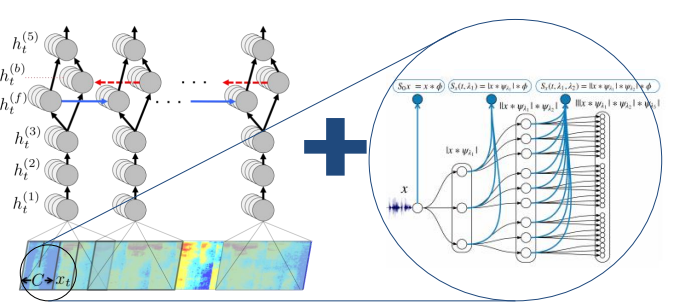
\includegraphics[width=14cm]{thesis/images/ctc_scatter.png}\\
  \caption{Deep scattering Bi-RNN Model} \label{fig_6_1_ctc_scatter}
\end{figure}

\section{CTC Decoding}

In chapter three the CTC loss function algorithm was established as being able to maximise the probability of two cases.  The first case of transiting to a blank and the second case of transiting to a non blank.  In this section, this concept is used to enable decoding of the network output from posterior distribution output to character sequences which can be measured against a reference transcription using either character error rate (CER) or word error rate (WER).

Recall, all the output symbols are in the alphabet $\Sigma$ and augmented with the blank symbol. The posterior output of the CTC network is the probability of the symbol given the speech feature input $p(c|x_t)$ at time $t$ for $t=1,\dots,T$ and $T$ is the length of the input sequence.  Also recall two further sets of probabilities also being maintained by the model are the probability of a blank character $p_b$ and that of a non blank character $p_{nb}$.

Several strategies have been employed to obtain a translation string from the output of the deep neural network.  The prefix beam search employed by the CTC decoder of this research is derived from an initial greedy approximation, where at each time step determine the argument that maximises the  probability $p(c|x_t)$ at each time step. Let $C=(c_1,\dots,c_T$ be the character string then, the greedy approach has 
\begin{equation}
    c_t=arg\max_{c\in\Sigma}p(c|x_t)
\end{equation}
However, this simple approximation is unable to collapse repeating sequences and remove blank symbols. In addition, the approximation is unable to include the constraint of a lexicon or language model.

The prefix beam search algorithm \cite{hannun2014first} adopted in this work incorporates a language model derived from a lexicon in addition to keeping track of the various likelihoods used for decoding.  For the language model constraint, the transcription $W$ is recovered from acoustic input $X$ at time $t$ by choosing the word which maximising the posterior probability:
\begin{equation}
W_i=arg\max_{W_i \in \Sigma_W} p_{net}(W;X)p_{lm}(W)
\label{eqn_c6_decoder01}
\end{equation}
In equation \ref{eqn_c6_decoder01}, the Bayes product of language model prior $p_{lm}$ and the network output $p_{net}$ are utilised to maximise the probability of a particular character-word sequence in the lexicon given by $\Sigma_W$.  The overall calculation used to derive the final posterior distribution includes word insertion factors ($\alpha$ and $\beta$) used to balance the highly constrained n-gram language model.

The second strategy adopted by the prefix beam search which improves the decoding algorithm is the beam search strategy.  With this approach, the search maintains all possible paths; however, it retains only $k$ number paths which maximise the output sequence probability.  Improvements gained with this method are seen when certain maximal paths are made obsolete owing to new information derived from the multiple paths in being maintained in memory. 

The recursive prefix beam search algorithm illustrated in Figure \ref{fig_c6_decoder01} attempts to find the string formulated in equation \ref{eqn_c6_decoder01}.  Two sets prefixes $A_{prev}$ and $A_{nxet}$ are initialised, such that at $A_{nxet}$ maintains the prefixes in the current time-step while $A_{prev}$ maintains only $k$-prefixes from the previous time-step.  Note that at the end of each time step $A_{prev}$ is updated with only -most probable prefixes from $A_{nxet}$. Therefore while,  $A_{nxet}$ contains all the possible new paths from based on $A_{prev}$ as a Cartesian product of $A_{prev} \times \Sigma \in \mathcal{Z}^k\times\mathcal{Z}^{|\Sigma|}$ where $|\Sigma|$ is the length of $\Sigma$. The probabilities of each prefix obtained at each time step are the sum of the probability of non-blank plus the probability of a blank symbol.
\begin{sidewaysfigure}[ht]
    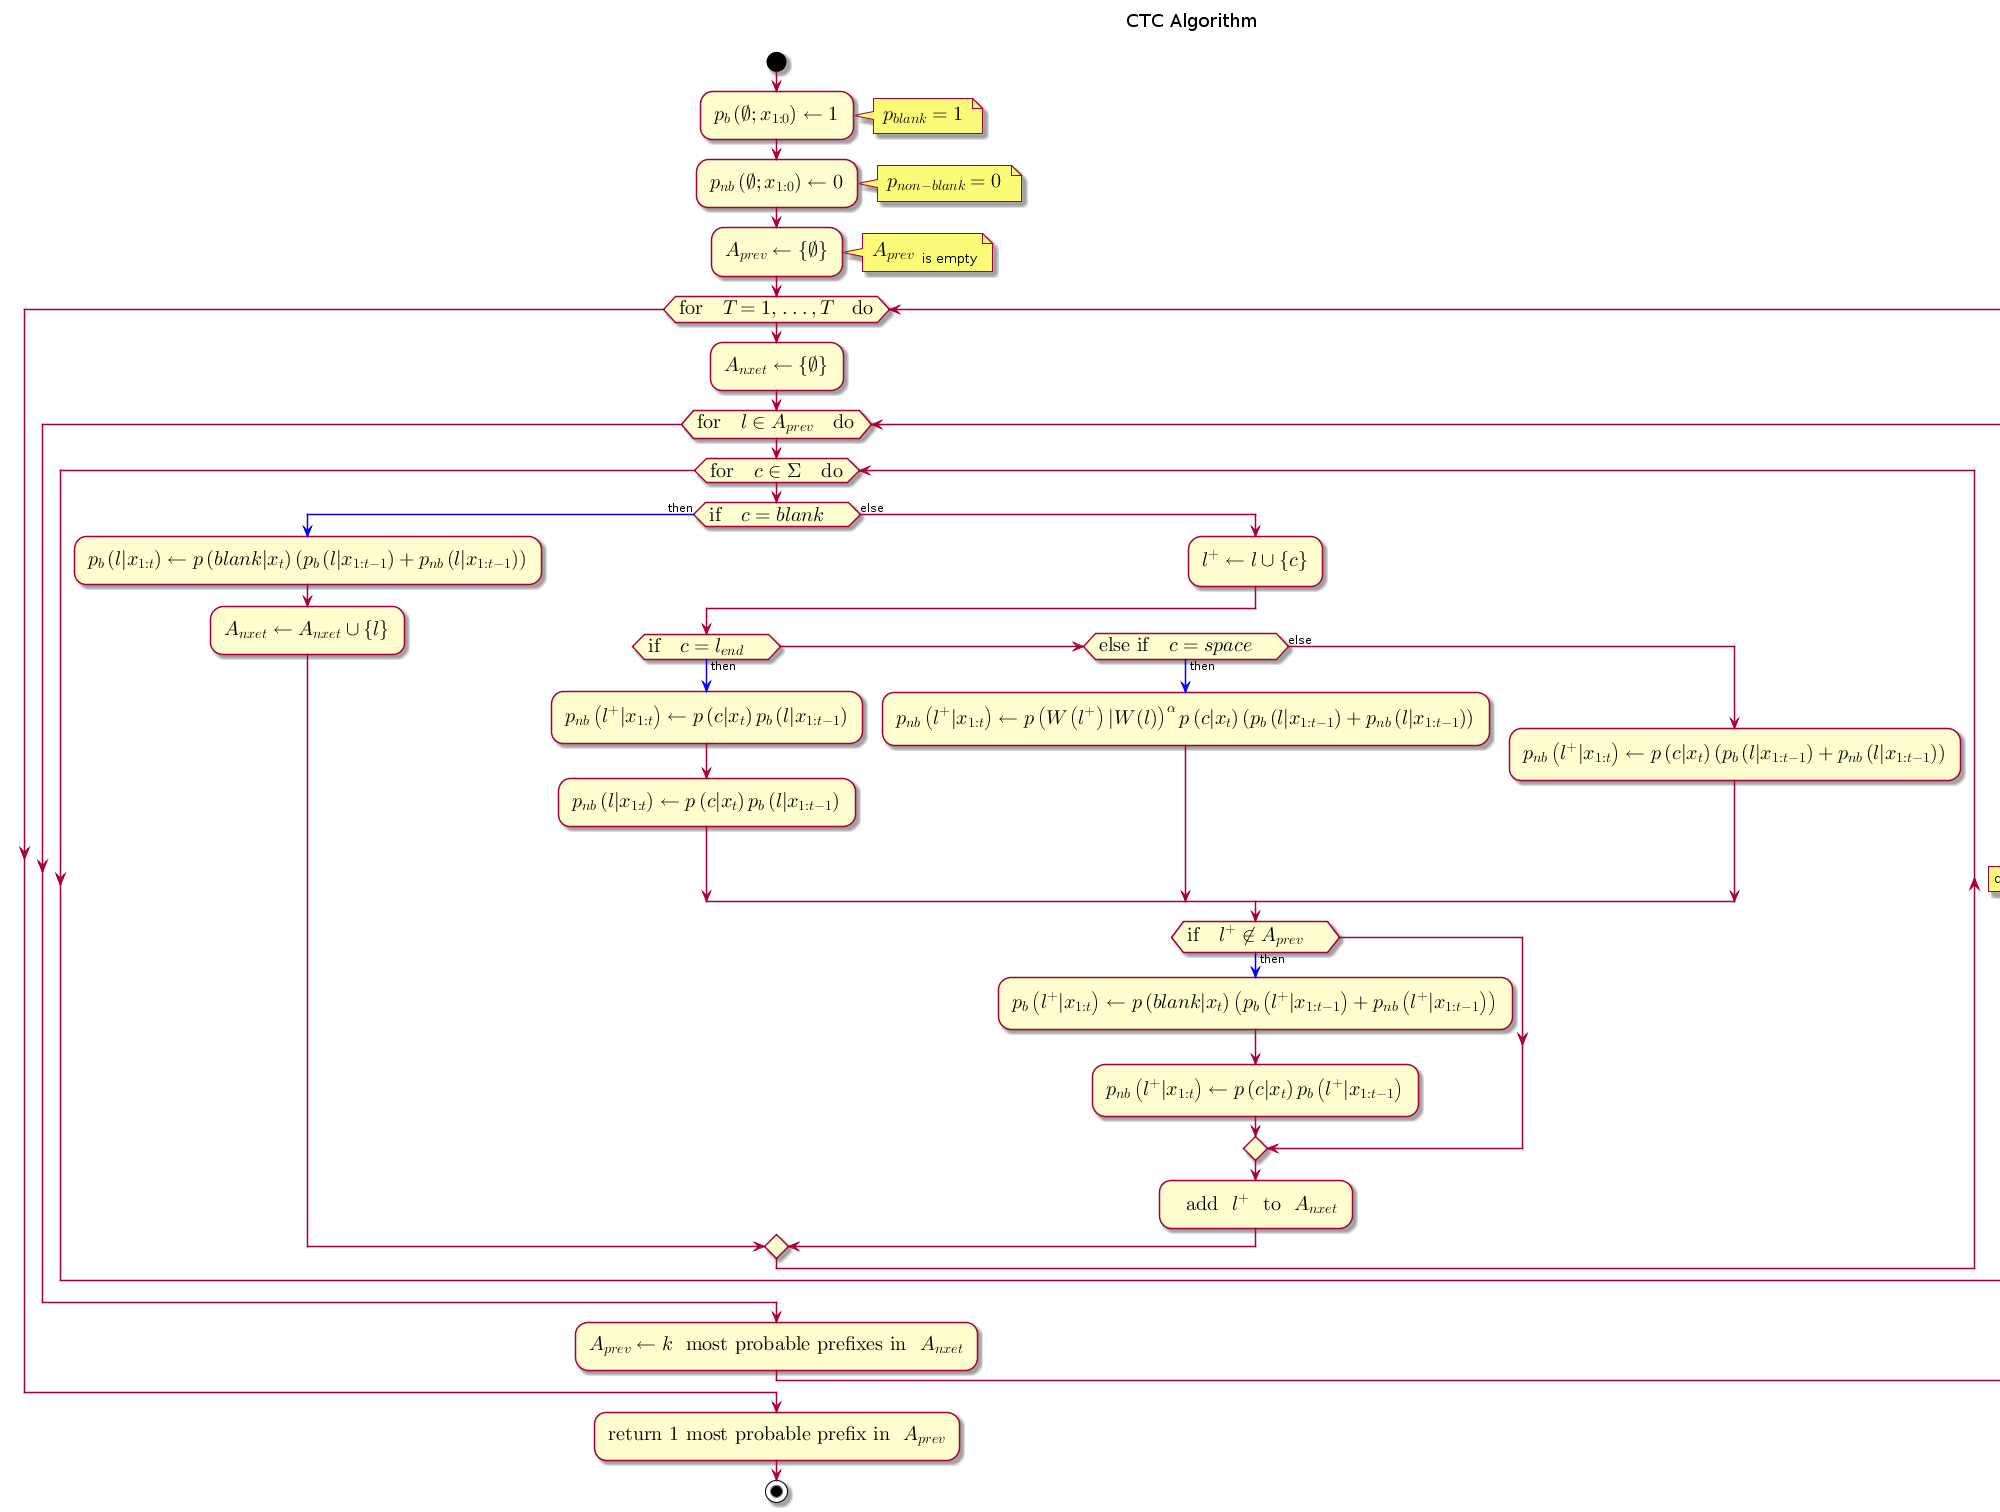
\includegraphics[width=22cm]{ctc}
    \caption{Prefix beam search algorithm}
    \label{fig_c6_decoder01}
\end{sidewaysfigure}

At every  time step and for every prefix $\ell$ currently in $A_{prev}$, a character from the alphabet $\Sigma$ is presented to the prefix. The prefix is only extended only when the presented symbol is not a blank or a space. $A_{nxet}$ and $A_{prev}$ maintain a list of active prefixes at the previous time step and proposed prefixes at the next time step respectively, The prefix probability is given by multiplying the word insertion term by the sum of the blank and non-blank symbol probabilities.
\begin{equation}
p(\ell|x_{1:t})=(p_{nb}(\ell|x_{1:t})+p_b(\ell|x_{1:t}))|W(\ell)|^\beta
\label{eqn_c6_decoder03}
\end{equation}

$W(\cdot)$ is obtained by segmenting all the characters in the sequence with the space-character symbol and truncating any characters trailing the  set of words in the sequence.  The prefix distribution however varies slightly depending on network output character being presented.

$\ell_{end}$ is the variable representing the last symbol in the prefix sequence in $A_{prev}$. If the symbol presented is the same as $\ell_{end}$ then the probability of a non-blank symbol,$p_{nb}=0$ . If the symbol being presented is blank then we do not extend the prefix.  Finally, if the symbol being presented is a space then we invoke the language model as follows
\begin{equation}
p(\ell^+|x_{1:t})=p(W(\ell^+)|W(\ell))^\alpha(p_{nb}(\ell|x_{1:t})+p_b(\ell|x_{1:t}))|W(\ell)|^\beta
\label{eqn_c6_decoder03}
\end{equation}

Note that $p(W(\ell^+)|W(\ell))$ is set to $0$ if the current word $W(\ell^+)$ is not in the lexicon. This becomes a constraint to enforce all character strings to consist only of words in the lexicon.  Furthermore,  $p(W(\ell^+)|W(\ell))$ is extended to include all the character sequences representing number of words considered by the n-gram language model by constituting the last $n-1$ words in character sequence $W(\ell)$.

\section{Model Hyper parameters}
The hidden layer matrix for each layer comprised 1024 hidden units (6.6M free parameters).  The weights are initialised from a uniform random distribution having a standard deviation of 0.046875.  The Adam optimisation algorithm \citep{kingma2014adam} was used with initial learning rate of, and a momentum of 0.95 was deployed to optimise the learning rate.

The network was trained for a total of five to fifty epochs over the training set for experiments conducted. The training time for Python GPU implementation is shown in Table \ref{tab_c6_01_training}.  For decoding with prefix search we use a beam size of $200$ and cross-validated with a held-out set to find optimal settings for the parameters $\alpha$ and $\beta$. Figure \ref{fig_6_3_wer} shows word error rates for various GPU configurations and audio data-set sizes.

\startblue
\section{BiRNN with Transducer+Attention end-to-end Architecture}\label{sec_7_5_blstm_t}

The end-to-end architecture at the core of ESPNet is the CTC-Transformer+Attention Transducer model.  Together these two architectures achieve joint multi-objective speech training and decoding.  The CTC-Transformer model is based on a Bi-RNN similar to what is obtainable in the DeepSpeech model.  There are up to 11 variants of Attention networks implemented in ESPNet, however, the results of the ESPNet experiment performed was determined from the model described in \cite{chorowski2015attention}.  Moreover, the multi-objective training was performed with equal weights on both the CTC-transformer and the Attention-Transducer.  Finally the system was trained for 20 epochs only.

With this minimal default setting, the test set had a final recognition score of 9.5\% character error rate (CER).  The next Chapter discusses how the baseline can be scaled and remodelled for integrating scattering features.

The inclusion of Attention-based models and the warp-CTC decoder implemented in ESPNet ensures faster convergence and ultimately faster time to train, in addition to the end-to-end architecture.  Using a weighting function  one can control how much bias either the CTC-Transform or the Attention-Transducer will get during training.  The joint training helps to improve robustness as well as achieve fast convergence.

\begin{equation}
    \mathcal{L}=\alpha\mathcal{L}^{ctc}+(1-\alpha)\mathacal{L}^{att}
    \label{eqn_c7_esp00}
\end{equation}

At the same time joint decoding of labels is integrated with the character based RNN-language modelling. The log probability of the RNNLM-integrated decoding of character labels is as follows

\begin{equation}
    \log p(y_n|y_{1:n−1},\mathbf{h}_{1:T‘})=\log p^{hyp}(y_n|y_{1:n−1},\mathbf{h}_{1:T‘})+\beta\log p^{lm}(y_n|y_{1:n−1})
    \label{eqn_c7_esp01}
\end{equation}
Where joint decoding, $\log p^{hyp}(y_n|y_{1:n−1},\mathbf{h}_{1:T‘})$ is given by
\begin{equation}
    \log p^{hyp}(y_n|y_{1:n−1},\mathbf{h}_{1:T‘})\\
    & = \alpha\log p^{ctc}(y_n|y_{1:n-1},\mathbf{h}_{1:T'})+(1-\alpha)\log p^{att}(y_n|y_{1:n-1},\mathbf{h}_{1:T'})
\end{equation}
Furthermore, multi-channel training allows noise robust and far-field speech recognition tasks which incorporates joint 83-dimension feature-training in addition to speech enhancement features such as beam forming and STFT masking \cite{ochiai2017multichannel}.

\section{Model Baselines}
The model baselines were trained alongside their scatter transform counterparts.  In addition, we adopted the model produced by the Mozilla DeepSpeech team.  This model had a similar architecture with 5 hidden units and 2048 hidden units.  This baseline was trained on Librespeech corpus and the common voice data corpora \citep{panayotov2015librispeech, ardila2019common}.   Study by \cite{hannun2014first} reported successful character error rate (CER)  using deep neural network (DNN), recurrent deep neural network with only forward temporal connections (RDNN), and also bi-directional recurrent neural networks (BRDNN). The models used in their study had 5 hidden layers having either 1,824 or 2,048 hidden units in each hidden layer.  

Word Error Rates obtained by this additional model were optimised after 75 epochs, learning rate of 0.0001 and a dropout rate of 15\%.  In addition, the language model hyper parameters for alpha and beta were 0.75 and 1.85 respectively.  This achieved 8\% WER. This model was developed using MFCC features of the training corpora.

\section{Model Simulations}

Speech model training experiments were carried out on the two different end-to-end models as well as on different \acrshort{gpu} configurations. The first set of experiments was performed for the \acrshort{birnn}-only model.  The first \acrshort{gpu} configuration for the \acrshort{birnn}-only model consisted of 2 \acrshort{gpu}s having a total of 10 gigabytes of memory. The second \acrshort{gpu} configuration comprised 5 \acrshort{gpu}s having a total of 15 gigabytes of memory. Experiments for the BiRNN end-to-end model with transducer and attention were also performed using a \acrshort{gpu} configuration having 4 gigabytes of memory. 

\subsection{\acrshort{birnn}-only end-to-end model Experiments}
For the \acrshort{birnn}-only end-to-end experiments, GPU configuration experiments were carried out on varying-size subsets of the common voice corpus.   The various GPU configurations along with the training times are shown in Table \ref{tab_c6_01_training}.

\begin{table}
  \caption{\acrshort{birnn}-only Experiments}
  \label{tab_c6_01_training}
\begin{tabular}{lccc}
\toprule
Experiment & Hours of speech & Total training time & Training status\\
\midrule
1. 2xGPU 10GB RAM & 1 & 7 days & Complete\\
2. 2xGPU 10GB RAM & 10 & 40 days & Not complete\\
3. 5xGPU 15GB RAM & 2 & 2 days & Complete\\
4. 5xGPU 15GB RAM & 40 & 40 days & Not complete\\
5. 1xCPU 16GB RAM & 20 & 20 days & Not complete\\
6. 1xGPU 2GB RAM & 20 & 20 days & Not complete\\
\bottomrule
\end{tabular}
\end{table}

It can be seen in Table \ref{tab_c6_01_training}, only two experiments had reached completion.    The others had to be stopped for exceeding reasonable training times of 20 and 40 days. Out of the four experiments that did not complete, all the GPU-based experiments had trained for up to 20 epochs and quantitative metrics were taken for these experiments.  Table \ref{tab_c6_02_training} shows the details for the \acrfull{wer} accuracy metrics for a total of four experiments. The number of hours of speech, corpus type and total number of epochs are also shown. Accuracy curves are shown in figure \ref{fig_6_3_wer}.

\begin{table}
  \caption{\acrshort{birnn}-only Experiments Summary}
  \label{tab_c6_02_training}
\begin{tabular}{lccccc}
\toprule
Experiment & Hours & Corpus & epochs & Metric & Score\\& of speech\\
\midrule
1. 2xGPU 10GB RAM & 1 & CV LVCSR & 40 & WER(\%) & 100+\\
2. 2xGPU 10GB RAM & 10 & CV LVCSR & 25 & WER(\%) & 100+\\
3. 5xGPU 15GB RAM & 2 & CV LVCSR & 40 & WER(\%) & 100\\
4. 5xGPU 15GB RAM & 40 &  CV LVCSR & 40 & WER(\%) & 87\\
\bottomrule
\end{tabular}
\end{table}


\begin{figure}
\centering
  % Requires \usepackage{graphicx}
  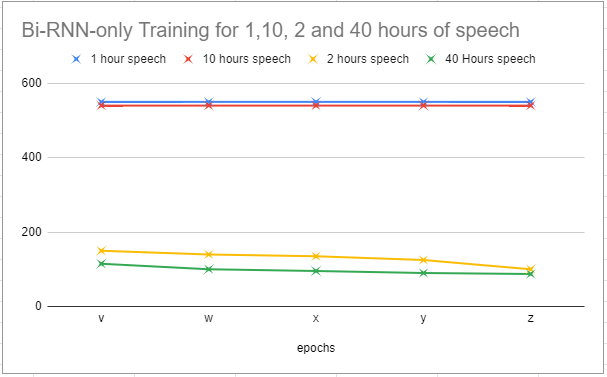
\includegraphics[width=14cm]{thesis/images/brnn_only.png}\\
  \caption{\acrshort{birnn}-only Experiments Error curve, where w\<x\<y\<z are taken arbitrarily across the total
number of epochs} \label{fig_6_3_wer}
\end{figure}


\subsection{\acrshort{birnn} with Transducer and Attention mechanism Experiments}
The \acrfull{espnet} \citep{watanabe2018espnet} provides building blocks for \acrshort{blstm} transducer with attention mechanism  described in Section \ref{sec_7_5_blstm_t}.  Two experiments involving a much smaller audio corpus guaranteed to converge quickly at training and a larger Italian language speech corpus \citep{foxvorge2019} used for these experiments.  The AN4 (alphanumeric) corpus by Carnegie Mellon University \citep{acero1990acoustical}, is a small vocabulary speech corpus having only 948 training utterances and 140 test utterances.

The speech corpora utterances are 16-bit linearly sampled at 16kHz, each recording made with near-field microphone quality.  The compressed tar file comes with a variety of audio formats including raw wav format, the NIST sphere format and those already encoded as Mel cepstral coefficients.

The end-to-end architecture at the core of ESPNet is the CTC-Transformer+Attention Transducer model.  Together these two architectures achieve joint multi-objective speech training and decoding.  The CTC-Transformer model is based on a \acrshort{blstm} and is similar to what is obtainable in the DeepSpeech model.  There are up to 11 variants of Attention networks implemented in \acrshort{espnet}, however, the results of the \acrshort{espnet} experiment performed was determined from the model described in \cite{chorowski2015attention}.  Moreover, the multi-objective training was performed with equal weights on both the CTC-transformer and the Attention-Transducer.  

\begin{table}
  \caption{\acrshort{birnn} with attention and transducer Experiments}
  \label{tab_c6_03_training}
\begin{tabular}{lcccc}
\toprule
Experiment & Hours & Training  & Epochs & Training \\
& of speech & time & & status \\
\midrule
1. 1xGPU 4GB (log mel.) & 1 & 15 minutes & 20 & Complete\\
2. 1xCPU 16GB (scatter feat) & 1 & 3 days & 100 & Complete\\
3. 1xGPU 4GB (log mel) & ~10 & 11 hours & 200 & Complete\\
4. 1xGPU 4GB (scatter feat) & ~10 & 38 hours & 200 & Complete\\
\bottomrule
\end{tabular}
\end{table}
Experiments were carried out using ESPNet default parameters which included those for character based-Recurrent Neural Network language model RNN-LM, multi-channel feature input and multi-objective learning using both CTC-Transformer and Attention-Transducer networks.

With this minimal default setting, the test set had a final recognition score of 9.5\% character error rate (CER).  The next Chapter discusses how the baseline can be scaled and remodelled for integrating scattering features.

\begin{table}
  \caption{\acrshort{birnn} with attention and transducer Experiments Summary}
  \label{tab_c6_04_training}
\begin{tabular}{lcccc}
\toprule
Experiment & Hours & Corpus & Metric & Score\\& of speech\\
\midrule
1. 1xGPU 4GB (log mel) & 1 & AN4 SVCSR & WER(\%) & 12.9\\
2. 1xGPU 4GB (scatter feat.) & 1 & AN4 SVCSR & WER(\%) & 26.8 \\
3. 1xGPU 4GB (scatter feat) & ~10 & Voxforge-italian (LVSCR) & WER(\%) & 76.7 \\
4. 1xGPU 4GB (log mel) & ~10 &  Voxforge-italian (LVSCR) & WER(\%) & 72.4\\
\bottomrule
\end{tabular}
\end{table}

\section{Model Results Interpretation}
Interpretation of Model Results
Experiments carried out to train the end-to-end \acrshort{asr} were performed on the following system configurations
\begin{enumerate}
    \item GPU (GTX1050) with 2GB RAM
    \item GPU (GTX1050) with 4GB RAM
    \item GPU (GTX1060) with 6GB RAM
    \item GPU (GTX1070) with 3GB RAM
    \item CPU with 16GB RAM
\end{enumerate}

\subsection{Bi-RNN-only experiment discussion}
Configurations with CPU were used as control experiments to compare the GPU efficiency with the CPU being compensated with more memory.  The higher memory allowed the CPU configurations to remain accessible during training unlike the GPU systems that used up most of the system resources bringing the computer system close to a grinding halt and making the GPU systems difficult to access while training was in progress.  In as much as a number of the experiments done exceeded 10 days, our goal was not to exceed more than 10 days training for speech models.  What the GPU lacked in memory resources was compensated for in computational speed gained due to their capacity for parallel.  By changing the batch size, memory resource requirement and computational parallelism was simultaneously managed for all experiments.  Therefore for CPU training computational speedup was attempted by increasing the batch size and for GPU training batch sizes were reduced so as not to quickly deplete the small memories.  For \acrshort{birnn}-only experiments, regardless of the batchsize allocations, only 2GPU configurations  (1 and 3 in Table \ref{tab_c6_01_training}) completed training for the given amounts of epochs and training data.

Table \ref{tab_c6_02_training} shows four GPU-only configurations.  These GPU training configuration experiments had completed at least 20 epochs.  Training metrics for these configurations are plotted in Figure \ref{fig_6_3_wer}.   A reduction in training loss is observed once the data was increased to two hours of training.  This gives an indication of the model learning on the amount of data given.  Even though the speech models were trained on English language only.  We can simulate low resource settings in the English language by limiting the amount of data available during training.  Moreover, word error rates (WER) only showed improvement on the 40 hours data set.  This also indicates that a threshold of about 40 hours is required for the model to begin to converge for a Large Scale Vocabulary Continuous Speech Recognition (LSVCSR) system

The results showed that the training of the model was moving towards a very slow convergence as indicated by the slow decrements in training loss.  Initial experiments were performed on single GPU Units.  Batch size settings for these experiments were very small to fit into the limited RAM sizes on the GPUs.  At a later stage, multi-GPU units were utilised as a strategy to speed up training by increasing the batch sizes to run on the combined memory.  This however did not result in the anticipated speed up. It is suspected that this outcome may have been as a result of latency copying model parameters between GPU units and CPU multiple times during training.

\subsection{Bi-RNN with Transducer and attention mechanism experiment discussion}
Results from Bi-RNN with Transducer and attention experiments had shown greater promise in terms of completion of training within the time constraints set. Results shown in table \ref{tab_c6_03_training} show that both CPU and GPU training completed training for less than 20 hours of training and total number of epochs.

We used a \acrfull{svcsr} corpus of English language and a \acrfull{lvcsr} of Italian and achieved a decent score of 26.8\% for the \acrshort{svcsr} corpus and a high error score of 76.7\% for the \acrshort{lvcsr} corpus.  The high error score for the \ref{lvcsr} from the observed results was attributed to the fact that the amount of data given ~10 hours is not sufficient for meaningful convergence.  This is also evidenced by the baseline result having a similar high error rate of 72.4\%.  A similar effect was also observed in the Bi-RNN-only experiments such that after training of 40 hours of data for 40 epochs the error was at 87\%.

From the training curves (Figures \ref{fig_6_2_loss} and \ref{fig_6_3_wer} however, we can see that at 40 epochs the Bi-RNN with transducer and attention mechanism experiments had a faster rate of convergence and this led to experiments being completed within the time limits set.

\section{Chapter Summary}

In this chapter the details of the combination of an end-to-end deep bi-RNN architecture and deep scattering features were elaborated on.  The architecture described follows a five-layer structure consisting of a feed-forward neural network in the first three layers and the last two consisting of recurrent structures flowing in two different directions.  A 250-dimension 2nd-order feature vector of deep-scattering encoding derived from a sampled raw audio file is fed into this network.

A second set of experiments comprising a similar architecture containing a \acrshort{bilstm} this time with encoder and decoder architectures and a transducer is also developed and tested.

The result showed the second set of experiments having the transducer architecture with attention mechanism are able to train faster but out of all the results, although some models came close to their respective baselines none actually performed better than the baseline models.  In Chapter \ref{ch8_future} we address ways that the results may be improved.

\stopblue

\begin{figure}
\centering
  % Requires \usepackage{graphicx}
  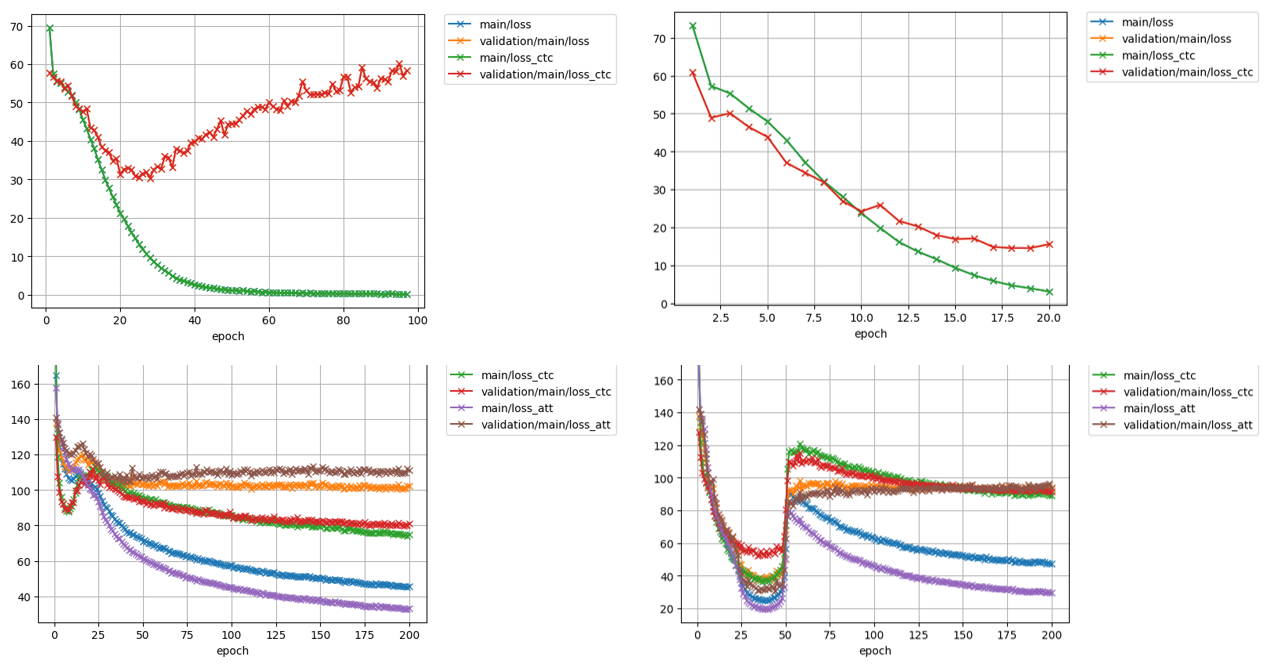
\includegraphics[width=14cm]{thesis/images/scatter_res.PNG}\\
  \caption{Training Loss, where $w<x<y<z$ are taken arbitrarily across the
total number of epochs} \label{fig_6_2_loss}
\end{figure}



\chapter{Future study}\label{ch8_future}
\textcolor{blue}{This research has been inspired by the notion of a \acrfull{llc}. One of the artificial intelligence tasks for \acrshort{llc} is \acrfull{asr}.  This research, therefore, explored the current advancements that have been made in the field of \acrshort{asr} and discovered one of the major challenges in field of \acrshort{asr} is that of new and low resourced languages.  In particular, considering \acrshort{asr} as a machine learning pipeline, this research favours a discriminative approach to \acrshort{asr} over generative approaches.  Although hybrid \acrshort{hmm}-\acrshort{dnn}, which is considered a generative model, does deliver state-of-the art results, the \acrshort{asr} pipeline involves training of different aspects of the \acrshort{asr} pipeline in separate processes.  The end-to-end approach, however, attempts to simplify this by offering a solution that involves training of a single discriminative "end-to-end" model. }

\startblue
As \acrshort{asr} is a machine learning pipeline,  the advancement of Machine Learning has had a direct impact on the development of more efficient speech recognition algorithms and at the same time the advancement of speech recognition helps with the improvement of Machine Learning algorithms, as in general, the methods used in Machine Learning usually are directly transferable to speech processing and vice-versa. This mutual relationship implies that speech recognition is a blossoming research field because there is a tremendous amount of work being done in the Machine Learning community. Particularly in the area of deep learning and neural networks, there is quite a vast array of neural network solutions that have been applied or are yet to be applied to speech recognition. This research examined the effect of using a different set of input features from the state-of-the-art log-mel features. Feeding these scatter transform features into end-to-end ASR DNN with the objective of a comparable fast and efficient speech recognition for new and low resource languages. The major advantage of our system is that in addition to robust end-to-end models coupled with unique front-end scatter transform features and the intrinsic integration of a character-based language model help to train low-resource languages for ASR in a resource efficient manner. 

This Chapter summarises the end-to-end and deep sequential models towards low-resource speech recognition developed by this research. In addition, additional models being developed in the research community which are closely related models are mentioned as areas of further research interest.  These include Generative Adversarial Networks (GANs) and Attention-based models. 

\section{Discussion of Output Research models}

Two well established key aspects of \acrshort{asr} from the \acrshort{asr} formulation in Equation \ref{eqn_2_3_bayes_sr} include an \acrfull{am} and a \acrfull{lm}. The objective of this research was to understand these key aspects \acrshort{asr} systems and develop \acrshort{asr} systems that can be accessible by new and or low resource languages.

The research objectives were met by developing speech models based on a neural network end-to-end approach. End-to-end discriminative neural network speech models have now become a well established method in Automatic Speech Recognition.   The Bi-directional Recurrent neural network (\acrshort{birnn}) end-to-end system, developed in this work, however, is augmented by features derived from a deep scattering network as opposed to the standard Mel Frequency Cepstral Coefficients(MFCC) features used in state of the art acoustic models.  These specialised deep scattering features, consumed by the \acrshort{birnn} model, represent a light-weight convolution network. 

\subsection{Main contribution to knowledge}
This work shows that it is possible to build a speech model from a combination of deep scattering features and a Bi-RNN. There has been no record of deep scattering features being used in end-to-end bi-RNN speech models as far as we are aware.  This thesis therefore demonstrates Deep Scattering features derived from wavelet filter operations on audio data produce viable candidates for end-to-end training of Automatic speech recognition models.

\stopblue
\section{Directions for future study}
\subsection{Generative adversarial networks (GAN)}

GANs consists of two Networks working as adversaries to one another.  The first, being a generative network, generates content.  The second network is a discriminative network intended to determine the accuracy of the first generative network.  Hence the generative network is generating output less distinguishable for the discriminator while the discriminator uses output from the generator to improve the ability to discriminate output from the generator with the original source data.

GAN networks can have applications where the generative network consists of a speech synthesis network and the discriminating network is  a speech recogniser.  However successive training of these two networks from a data-resource perspective would require an immense amount of data resources for expected performances. 

\subsection{Attention-based Models}

The objective of attention-based networks highlighted by  \cite{vaswani2017attention} is to reduce sequential computation while attaining hidden representation across arbitrary lengths of sequential input. Mechanisms which have been deployed to achieve this includes a combination of convolutional and recurrent schemes \citep{kaiser2016can,kalchbrenner2016neural, gehring2017convolutional}. \cite{vaswani2017attention} introduces a transduction model known as a Transformer based on self attention network with the ability to compute long term dependencies while eliminating sequence aligned RNN and convolutional architectures.

Self attention is a network that intrinsically reduces the need for intensive resource training.  \cite{vaswani2017attention} reports that state of the art BLEU score of 41.0 having used a small fraction of training resources.  While GANs might not be attractive for low resource speech recognition, they still remain an important tool for verification of the output of other networks.  At the same time self attention networks can help to reduce the resource requirements of GANs when used within the context of a GAN.

As a study to further this thesis, these networks are likely candidates for network training using scatter features as input discriminatory functions.  Attention based networks as a means reduce training resources required, while GANs can be used as a means to generate training data.


\subsection{Model Pretraining}
The major setback this work suffered was from a reasonable time for training.  This work therefore recommends that speech models or indeed artificial intelligence models should be trainable within a maximum of 30 days and shouldn't generally exceed 20 days training.

An area of neural network training optimisation not developed in this report is that of layer-wise greedy pre-training.  In this process, rather than train the deep neural network structure all in one stage, the network layers are successively added and trained layer by layer, one layer at a time \citep{Goodfellow-et-al-2016}.  The intuition behind this is that this makes the layers saturate much faster as the previous layer has already been saturated before the new layer is being added.

This layer-wise pretraining procedure is thought to speed up training, than training when done with the fully connected network and there have been a few different approaches to pretraining in for deep neural network architectures for speech recognition. 

\cite{hendrycks2019using} introduces an advanced pretraining method in which existing models are retrained in a Generative Adversarial Network (GAN) fashion in order to optimise performance and model robustness.  This is an instance where GANs are being deployed in speech recognition.  This method however is not likely going to help improve model training convergence time.

Another method described in \citep{ramachandran2016unsupervised,} uses a knowledge transfer mechanism where hidden layers in an already existing related network is re-trained with new extended layers to complete training in the new domain.  The effectiveness of such a transfer method will be measured of the how the two domains correlate with one another. It therefore, would be logical to conclude that the more the domains correlate the faster the pretraining model is likely to converge faster.

Finally, \cite{wang2019bridging} proposes a Tandem Connectionist Encoding Network (TCEN) for bridging the gap for fine tuning CTC-Transformer networks along with pretraining of Attention-transducers.

As a further study, amongst other techniques, the most viable method for this study is to investigate the knowledge transfer mechanism by approaching the feature engineering problem as a latent space analysis problem.  Given that during the process of mapping acoustic speech sequences to the MFCC reduced the latent space from a high dimension to a low dimension.  It is reasonable therefore to hypothesize that training from hidden layers of an MFCC deep RNN would converge faster than weights initialised through generic means.

\startblue
\section{Conclusion}

The outcome of this research is an \acrshor{asr} system which facilitates fast and efficient speech recognition using the end-to-end speech recognition and deep scattering speech features.  Another advantage of our \acrshort{asr} system was the intrinsic integration of a character-based language model enabling it to satisfy both low-resource challenge criteria of top level word and sentence modelling through the character-based language model and the sub-word and acoustic modelling of input features.

The word error rates obtained by our model with different data sizes and speech corpora was not as good as the features using log-mel features. However, the results were competitive 
 
\stopblue




\spacing{1.0}
\addcontentsline{toc}{chapter}{Appendix I - Haar wavelet}
\chapter*{\appendix}
\section*{Appendix I - Haar Wavelet}

A fundamental purpose of analysing functions such as the Fourier and wavelet functions are the reconstruction of signals from it’s decomposition.  Certain criteria or properties are therefore required for analysis functions.  

In Chapter \ref{c4_fourier}, the orthogonal properties of the Fourier transform equations was introduced.  In the case of wavelets the following properties ensue.  In addition to orthogonal properties, wavelets are required to perform localised analysis of a function. Hence, unlike their Fourier counterparts, they need to be bounded in time.  It is also seen that when the energy contained within the wavelet bases sum to zero (sometimes normalised to 1)i.e.
\begin{equation}
    E=\int_{-\infty}^\infty |x|^2dt=||x(t)||^2=0
    \label{app1_01_pwr}
\end{equation}

Then, such wavelet bases are orthonormal and the fundamental or scaling equation forms a recurrence relation which is a solution to the dilation equation as follows:
\begin{equation}
    \phi(t)=\sum_kc_k\phi(2t-k)
    \label{app1_02_dilation}
\end{equation}

Where $\phi(2t-k)$ is a contracted version of $\phi(t)$ shifted along the time axis by an integer step $k$ and factored by an associated coefficient $c_k$.  At the same time it is also observed that it is possible to setup this recurrence relation to becoming dyadic such that the sum of coefficients, $c_k$ equals $2$, i.e. $\Sigma_kc_k=2$. Haar, wavelets constitute the simplest of this family of wavelets.

The mother wavelet of the Haar wavelet has only two coefficients $c_0=c_1=1$ and is given by:
\begin{equation}
    \psi(t)=\phi(2t)+\phi(2t-1)
    \label{app1_03_mwavlet}
\end{equation}

Observe here that $c_0+c_1=2$, i.e. dyadic.  The solution to this recurrence equation and the resulting plot is given in Figure \ref{haar}. 

Through multi-resolution analysis, the following reconstruction of the Haar wavelet is derived:

\begin{equation}
   \phi_{j,k}[n]=2^{j/2}\phi[2^jn-k]
    \label{app1_04_mres}
\end{equation}

The parameter $j$, controls the resolution of the signal reconstruction and the following wavelets and function representation are given in Figure \ref{multires}
\label{app_haar}
\addcontentsline{toc}{chapter}{Appendix II - Gabor and Morlet wavelet filters}
\chapter*{\appendix}
\section*{Appendix II - Gabor and Morlet Wavelets}
\subsection*{Gabor Wavelet filter}
The 1D-Gabor wavelet is defined spatially by
\begin{equation}
    \psi(x)=exp\left(-\frac{x^2}{2\sigma^2}+i\xi x\right)
    \label{eqn_app2_wfil00}
\end{equation}
The Fourier-transform is
\begin{equation}
    \hat{\psi}(\omega)=exp\left(-\frac{\sigma^2(\omega-\xi)^2}{2}\right)
    \label{eqn_app2_wfil01}
\end{equation}
It's value bounded at 0 is $\hat{\psi(0)}=exp(-\sigma^2\xi^2/2)$, so we have
\begin{equation}
    \xi\sigma=\sqrt{-2\log(\hat{\xi}(0))}
    \label{eqn_app2_wfil02}
\end{equation}
The wavelets are therefore computed as 
\begin{equation}
    \psi_j=\frac{1}{a^j\sigma}\left(\frac{x}{a^j}\right)
    \label{eqn_app2_wfil03}
\end{equation}

Where $a$ is the scale factor.  if we call $\tau$, the value of the two Gabor where the plots intersect, we have, as in figure \ref{fig_app2_gab}.
\begin{figure}
\centering
  % Requires \usepackage{graphicx}
  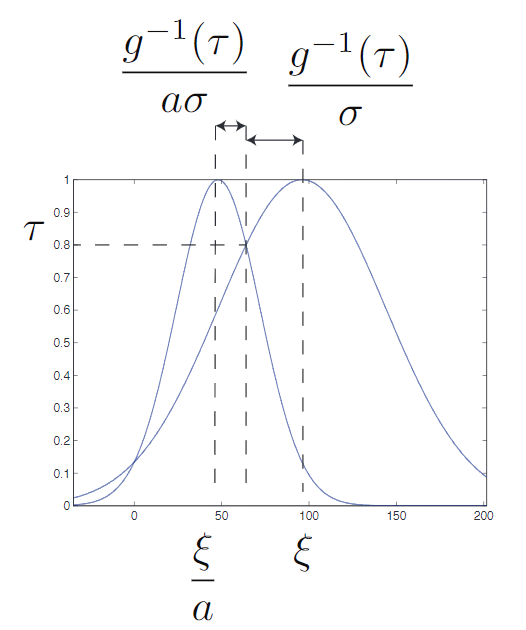
\includegraphics[width=14cm]{thesis/images/gab}\\
  \caption{Two-Gabor Plots showing $\tau$} \label{fig_app2_gab}
\end{figure}
\addcontentsline{toc}{chapter}{Appendix III - Scatter Transform implementation}
\chapter*{\appendix}

\section*{Appendix III - Matlab listing for scattering network}
\begin{lstlisting}[language=Matlab]
function scatter()
    %UNTITLED Summary of this function goes here
    %   Detailed explanation goes here
    T = readtable('data/cv-valid-dev.xlsx','ReadRowNames',true);
    F=table2cell(T(:,{'scatterc','wav_filename'}));
    all_files=size(F,1);
    ofm='hh:mm:ss';
    ifm='dd-mmm-yy HH:MM:SS.FFF';
    tic;
    for i = 1:all_files
      wav_file=strjoin(F(i,2));
      dss_file=strjoin(F(i,1));
      if exist(wav_file,'file')>0
      	if exist(dss_file,'file')==0
        	st = transpose(scatter_audio(wav_file));
        	csvwrite(dss_file,st);
      	end
      else
      	fprintf('\nNot found:%s',wav_file);
      end
 
      pg=i/all_files*100;
      ts=datestr(now,ifm);
      tv=toc;
      d=duration(seconds(tv),'Format',ofm);
      pc=(all_files/i*tv)-tv;
      eta=duration(seconds(pc),'Format',ofm);
 
      if mod(i,500)==0 || i==1 || i==10 || i==100
      	fileID = fopen('log/dss180625.log','w+');
      	s=sprintf('\n%s: processing file  %s',ts,wav_file);
      	fprintf(fileID,'%s',s);
      	fprintf('%s',s);
      	s=sprintf('\n%s : processing %d of %d files  %3.2f%% complete.. time elapsed = %s, eta = %s',ts,i,all_files,pg,d,eta);
      	fprintf(fileID,'%s',s);
      	fprintf('%s',s);
      	fclose(fileID);
      end
    end
end
 
function st= scatter_audio(inputArg1)
    y=audioread(inputArg1);
    N=length(y);
    T=2^9;
    filt_opt=default_filter_options('audio',T);
    Wop=wavelet_factory_1d(N,filt_opt);
    S=scat(y,Wop);
    S=renorm_scat(S);
    S=log_scat(S);
    st=format_scat(S);
end

\end{lstlisting}
\addcontentsline{toc}{chapter}{Appendix IV - Sample TensorFlow Client code}
\chapter*{\appendix}

\section*{Appendix IV - Code listing for Section \ref{sec_c3_tfw} - Sample TensorFlow client code}
\begin{lstlisting}[language=Python]
#!/usr/bin/env python
# -*- coding: utf-8 -*-
""" A one-hidden-layer-MLP MNIST-classifier. """
from __future__ import absolute_import from __future__ import division
from __future__ import print_function
# Import the training data (MNIST)
from tensorflow.examples.tutorials.mnist import input_data
import tensorflow as tf

# Possibly download and extract the MNIST data set. 
# Retrieve the labels as one-hot-encoded vectors. 
mnist = input_data.read_data_sets("/tmp/mnist",one_hot=True)

# Create a new graph
graph = tf.Graph()

# Set our graph as the one to add nodes to
with graph.as_default():

  # Placeholder for input examples (None = variable dimension)
  examples = tf.placeholder(shape=[None, 784], dtype=tf.float32)
  # Placeholder for labels
  labels = tf.placeholder(shape=[None, 10], dtype=tf.float32)
  
  weights = tf.Variable(tf.truncated_normal(shape=[784, 10],
    stddev=0.1))
  bias = tf.Variable(tf.constant(0.1, shape=[10]))
  
  # Apply an affine transformation to the input features
  logits = tf.matmul(examples, weights) 
    + bias estimates = tf.nn.softmax(logits)
  
  # Compute the cross-entropy
  cross_entropy = -tf.reduce_sum(labels * tf.log(estimates),
    reduction_indices=[1]) 
  # And finally the loss
  loss = tf.reduce_mean(cross_entropy)
  
  # Create a gradient-descent optimizer that minimizes the loss.
  # We choose a learning rate of 0.01
  optimizer = tf.train.GradientDescentOptimizer(0.5).minimize(loss)
  
  # Find the indices where the predictions were correct
  correct_predictions = tf.equal( 
    tf.argmax(estimates, dimension=1), 
    tf.argmax(labels, dimension=1))
  accuracy = tf.reduce_mean(
    tf.cast(correct_predictions, tf.float32))
    
with tf.Session(graph=graph) as session: 
  tf.initialize_all_variables().run() 
  for step in range(1001):
    example_batch, label_batch = mnist.train.next_batch(100)
    feed_dict = {examples: example_batch, labels: label_batch}
    if step % 100 == 0:
      _, loss_value, accuracy_value =
        session.run([optimizer, loss, accuracy], feed_dict=feed_dict)
      print("Loss at time {0}: {1}".format(step, loss_value))
      print("Accuracy at time {0}:{1}".format(step, accuracy_value))
    else:
      optimizer.run(feed_dict)
\end{lstlisting}\label{app4_tfcode}
\bibliographystyle{plainnat}

\bibliography{bib}

\end{document}
